\documentclass[a4paper, 12pt]{report}
\usepackage{graphicx} % Required for inserting images
\usepackage[T1]{fontenc}
\usepackage[latin1]{inputenc}
\usepackage{glossaries}
\usepackage{graphicx}
\usepackage{amsfonts}
\usepackage[hidelinks]{hyperref}
\usepackage{pifont}
\usepackage{eufrak}
\usepackage{amssymb}
\usepackage{listings}
\usepackage{amsthm}
\usepackage{matlab-prettifier}
\usepackage{pifont}
\usepackage{multicol}
\usepackage{verbatim}
\usepackage{tikz}
\usetikzlibrary{shapes,arrows}
\usepackage{tikz}
\tikzstyle{mybox} = [draw=black, thin, rectangle, rounded corners, inner ysep=5pt, inner xsep=5pt, fill=blue!15]
\newtheorem{theorem}{Theorem}

\usepackage{cleveref}
\usepackage[a4paper, top=2.8cm , bottom=2cm , right=2cm , left=2cm ]{geometry}

\title{
    {\color{black}
    \textbf{  \Huge{  LABORATORY OF
    ROBUST IDENTIFICATION AND CONTROL } }\\}
    \textit{Lecture notes}
    \linespread{2}
}
\author{Carlo Migliaccio}
\date{AA 2024/2025}

\theoremstyle{definition}
\newtheorem{definition}{Definition}[section]

\theoremstyle{remark}
\newtheorem*{remark}{Remark}

\pagestyle{headings}
\setcounter{MaxMatrixCols}{20}

\begin{document}
\maketitle
\tableofcontents


\part{Set-Membership System Identification}
\chapter{Introduction}

The \textit{first step} of any control problem is tipically the derivatin of a \textbf{mathematical model} for the plant to be controlled that without loss of generality is a \textbf{mechatronic system}. This is the most critical step because, assuming that we use physics laws:
\begin{itemize}
    \itemsep-0.1em
    \item We use \textit{simplifying assumptions}; 
    \item The value of the physical parameters involved in the equations (eg. mass, friction coefficients...) are not exactly known.
\end{itemize}
This fact is critical since \textit{standard} approaches to controller design are \textbf{model based}, in the sense that the controller is designed by strongly relying on the mathematical model used to describe the mechatronic system under study. Clearly the neglection of some aspects, will result in a neglection of state variables! For example for certain problems the assumption of \textit{rigid body} is satisfactory only under certain conditions.
\textbf{How to solve this problem?} If we compare the two common approaches for designing a controller (state space or  frequency description) the one based on frequency is much more able to face the problem of uncertainty.\\
In general, we can say that a controller is \textbf{robust} if it keeps good performances under the assumption of \textit{uncertain description}. For this reason we need a \textbf{robust description} of the plant that, roughly speaking, is made up of a \textbf{nominal model} and by a model for the \textbf{uncertainty}{\footnote{
    This can be modeled in an \textit{unstructured} or \textit{structured} way.
}}. Once such a model is derived we can apply some \textit{robust control techniques} for designing a controller  ($\mathcal{H}_{\infty}$, $\mu$-synthesis...)\\

In order to deal with the presence of the uncertainty and to overcome the limitations related to the first principle modeling approach we will focus on \textbf{System Identification (SysId)} (Part I)  and \textbf{Direct Data Driven Controller design (DDDC)} (Part II).

\section{Mathematical modeling of dynamical systems}
Since we have discussed about the importance of the mathematical model, now we can give an overview of the approaches one can track. 
\subsection{White-Box modeling \textit{(first principles)}} The models deriving from \textbf{white-box approach} are obtained by applying the first principle of physics and all the physical phenomena involved in the equation, also all the \textit{physical parameters} involved in the equation are \textbf{assumed to be exactly known}. The main idea which is useful to stress is that here \textbf{we know everything including the physical parameters}. 

\subsection{Gray-Box modeling}
They are models based on equations obtained (again) by applying first principles, but this time the parameters entering the equations are not exactly known and so an estimation procedure from experimantally collected data is needed. 

\subsection{Black-Box modeling}
In this case the structure of the equation is selected by the user on the basis of some "general" \textbf{a-priori information} on the system physics (eg. linearity). The parameters involved in the equation of the black-box model are then estimated/computed by using experimentally collected data. In general the parameter of a black box model do not have any \textit{physical meaning}.

\subsection{Some comments on the three approaches}
White-box models are not very useful in practice, where is very irrealistic the fact of having the knowledge of everything! Instead, more interesting is the comparison between \textbf{Gray-box} and \textbf{Black-Box} models. In both cases we have \textit{some information} (physical insights) and use the data in order to estimate the parameters themselves.

In \textbf{gray-box modeling} the structure of the equations is not selected by the user since it is forced by the first principle approach. For this reason in general the equations of a gray-box will depend in a \textbf{possibly complx nonlinear} way from the physical parameters to be estimated.

\subsubsection{Example 1 (GRAY-BOX)}
Let us assume that we know the plant to be modeled is an LTI one. You will remember that in the state-space representation, one can represent a dynamical system as:
\begin{equation*}
    \begin{aligned}
        \dot{x}(t)=Ax(t)+Bu(t)\\
        y(t)=Cx(t)+Du(t)
    \end{aligned}
\end{equation*}
If we look inside the $A$ matrix for example we can find:
\begin{equation*}
    A=\begin{bmatrix}
        \frac{m}{k^2}&\sqrt{\beta}\\
        \alpha^2\frac{k^3}{\gamma}&\gamma^2
    \end{bmatrix}
\end{equation*}
The mathematical procedure for the estimation of the parameters will be complex since they appear in the equation in a non linear way. Then, the modeling of such a plant will become very hard. This represents the main limitation of the gray-box approach. \\

\vspace{1cm}
\noindent
On the other hand, in the \textbf{black-box approach}, we have more freedom to select the structure of the equations, especially because we do it in a \textit{more convenient way} by only exploiting some general properties derived from our physical insights.

Coming back to the example we have just seen, the matrix $A$ will be made up of four coefficients $a_{ij}$ which appear linearly in the equation. The main difference is that such coefficients do not have a physical meaning.

\section{Steps for mathematical modeling}
The procedure we have for obtaining the mathematical model  is the following:
\begin{enumerate}
    \item \textsf{\textbf{STEP 1}} Exploit available \textit{a-priori information} on the system under study to select the structure of the mathematical equations describing the Input-Output mapping. In the most general case we do not know all the state variables, from this fact we can understand that we derive an \textbf{input-output model} (equation) for the plant like the following:
    \begin{equation}
        \underbrace{y(t)}_{\textsf{output}}=
        f( \underbrace{u(t)}_{\textsf{input}}, \underbrace{\theta}_{\textsf{parameters}})
    \end{equation}
    \item \textsf{\textbf{STEP 2}} Collect Input-Output data representing the behaviour of the system under study by performing an (open-loop) experiment. In particular, we collect the output $\tilde{y}$ from the plant using as input the sequence $\tilde{u}$.
    \item \textsf{\textbf{STEP 3}} To formulate a suitable \textbf{mathematical problem} to estimate/compute the values of parameter $\theta=[\theta_1...\theta_n]^T$ in such a way that our mathematical model is going to describe the behaviour of the real system, \textbf{as well as possible (in some sense)}. A common approach is to compute the parameter by solving the following problem:
    \begin{equation} \label{eq:problem}
        \hat{\theta} = \arg\min_{\theta}{J(\theta)}
    \end{equation}
    where $\hat{\theta}$ is the vector of parameters to be estimated, while $J(\theta)$ is the functional to be minimized. Usually we take it as $J(\theta)=\Vert \tilde{y}-f(\tilde{u}, \theta)\Vert$.
    At this stage the difference between gray-box and black-box approach models comes into play, since:
    \begin{itemize}
        \item \textbf{Gray-box models} $\Longrightarrow$ $f(\tilde{u}, \theta)$ will depends by a complex nonlinear function from $\theta$ (parameters); 
        \item \textbf{Black-box models} $\Longrightarrow$ $f(\tilde{u}, \theta)$ will be selected by the user in order to depend linearly from $\theta$ (if possible) or anyway in the \textit{simplest possible way}.
    \end{itemize}
\end{enumerate}

\section{Gray-Box vs Black-Box}
We have said that in the case of \textbf{Gray-box models} in general $f(u,\theta)$ may be a \textit{nonlinear} and \textit{non convex} function of $\theta$. This imply that the problem (\ref{eq:problem}) is going to be a \textbf{non convex optimization problem}, and in this case it is not trivial to solve it, the best I can say is to find \textbf{local minima}. In some situations we could be particularly lucky, and choosing a particular initial point there is the possibility of finding  the global minimum. However there is no way to certify it! Clearly a local minima, could correspond to a bad estimate of the parameter $\theta$.

\begin{figure}[h]
    \centering
    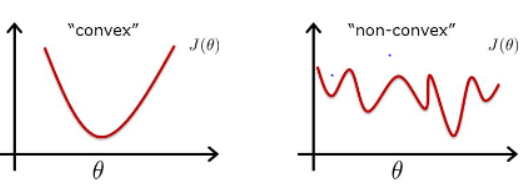
\includegraphics[scale=1]{img/cvx_nocvx.png}
    %\caption{Convex vs Non-Convex }
\end{figure}

For \textbf{Black-box} models, by selecting the parametrization of $f$ such that it could be a \textbf{convex function of $\theta$}, the problem \ref{eq:problem} becomes a \textbf{convex optimization problem}. In 1D the functional to be minimized is something similar to the one showed in the figure above. Convex functions have a  unique \textbf{global minima},there is no chance to be trapped in a local minima as in the non convex case. Clearly, waht is missed in this kind of approach is the \textit{physical meaning} of the estimated parameters. Let us give an example to better clarify this aspect: 

\subsubsection{Example (Second-order LTI system)}
Suppose that from first principles of physics we derive the following transfer function:
\begin{equation*}\label{eq:nonlinear}
    H(s)=\frac{
        \frac{p_1^2}{p_2}s+\frac{p_3}{\sqrt{p_4}}
    }{
        s^2+\frac{p_1p_4}{p_3^2}s+1
    }
\end{equation*}
where $p_1, ..., p_4$ are physical (meaningful) parameters. What does we miss by modeling the transfer function by using the following model derived for example after a \textit{black-box procedure}?
\begin{equation*}
    H(s)=\frac{\theta_1{s}+\theta_2}{s^2+\theta_3{s}+\theta_4}
\end{equation*}
The physical meaning is clearly missed, but in many situation the objective is not to be grasped to the physical meaning of the parameters taken singularly, but (a) to derive an I/O model for the plant; (b) to use such a model for designing a (model-based) controller.\\

\noindent
In order to conclude this discussion we can say that:
\begin{itemize}
    \item The \textbf{black-box approach} is the \textit{best choice} when we want either to simulate the I/O behaviour of the system or to design a \textbf{feedback control system}; an important remark to do is that the \textbf{structure} of a such a model must be selected by exploiting the most important a-priori information on the system (eg. \textbf{linearity}, \textbf{time invariance}...)
    \item The \textbf{gray-box approach} is the \textit{best choice} when we want to estimate the values for some \textbf{physical parameters}.
\end{itemize}
\noindent 
It is true that -- in all the approaches can be used for \textbf{System Identification} -- the experimental data plays a crucial role, but also the \textit{a-priori information} are of paramount importance. Besides, given the experimentally collected data there is an infinite number of functions which can interpolate those data. But if we apply an arbitrary input and then we compare the estimated output with the true one, we can confirm that the derived function just overfits the provided data. Conclusion: together with \textit{a-posteriori information} (collected data), we need also the \textit{a-priori information}, otherwise a well SysId procedure cannot be performed.



\chapter{System Identification: Least Squares Approach}

We have introduced in the first chapter the concept of \textit{System Identification} and we caught the importance of experimentally collected data, clearly in this more or less complex procedure one has to take into account that since that -- the data are collected by performing experiments on the real plant, they can be affected by \textbf{uncertainty/measurement noise}.\\
Moreover, even if the system to be identified  is a \textbf{continuous-time one} the most natural model for SysId is the discrete-time one, since samples of continuos time signals are collected.

\section{Regression form for describing dynamical systems}
There are evidences that -- in a quite general manner -- any dynamical system can be represented by using the so-called \textbf{regression form}, which stabilizes a relation between the current output, the input samples and the samples of the previous output. It is defined as follows:
\begin{equation}    \label{eq:reg_form}
    y(k)=f(y(k-1), y(k-2),  ..., y(k-n), u(k-1), ..., u(k-m), \theta)
\end{equation}
For any physical system $m\le{n}$ where $n$ is the system order that is the number of \textit{state variables}.

\section{Error-in-variables(EIV): General setting for SysId}
The most general setting describing an experiment performed on a plant to be identified is the \textbf{Error-in-variables (EIV)}, here both output $y(k)$ and input $u(k)$ are affected by measurement noise $\eta(k)$ and $\xi(k)$ respectively. Then the collected data can be represented by:
\begin{align} 
    &\tilde{u}(k) = u(k) + \xi(k)\\
    &\tilde{y}(k) = y(k) + \eta(k)
\end{align} 
In some situation the sequence input $u(k)$ can be assumed to be perfectly known so $\xi(k)=0$, because we build it in order to stimulate the system.\footnote{
    Later, when the concept on noise will be better formalized, we will give to such an approach the name of \textbf{output error (OE)}.
}
However, the \textbf{EIV} is more general and encapsulate also the situation in which the system to be identified is a subsystem from a more complex plant, then, since both $u(t)$ and $y(t)$ must be measured, both input and output are corrupted  by uncertainty/measurement noise. 

The following is a figure that shows schematically the setting we have just described: 

\begin{figure}[h]
    \centering
    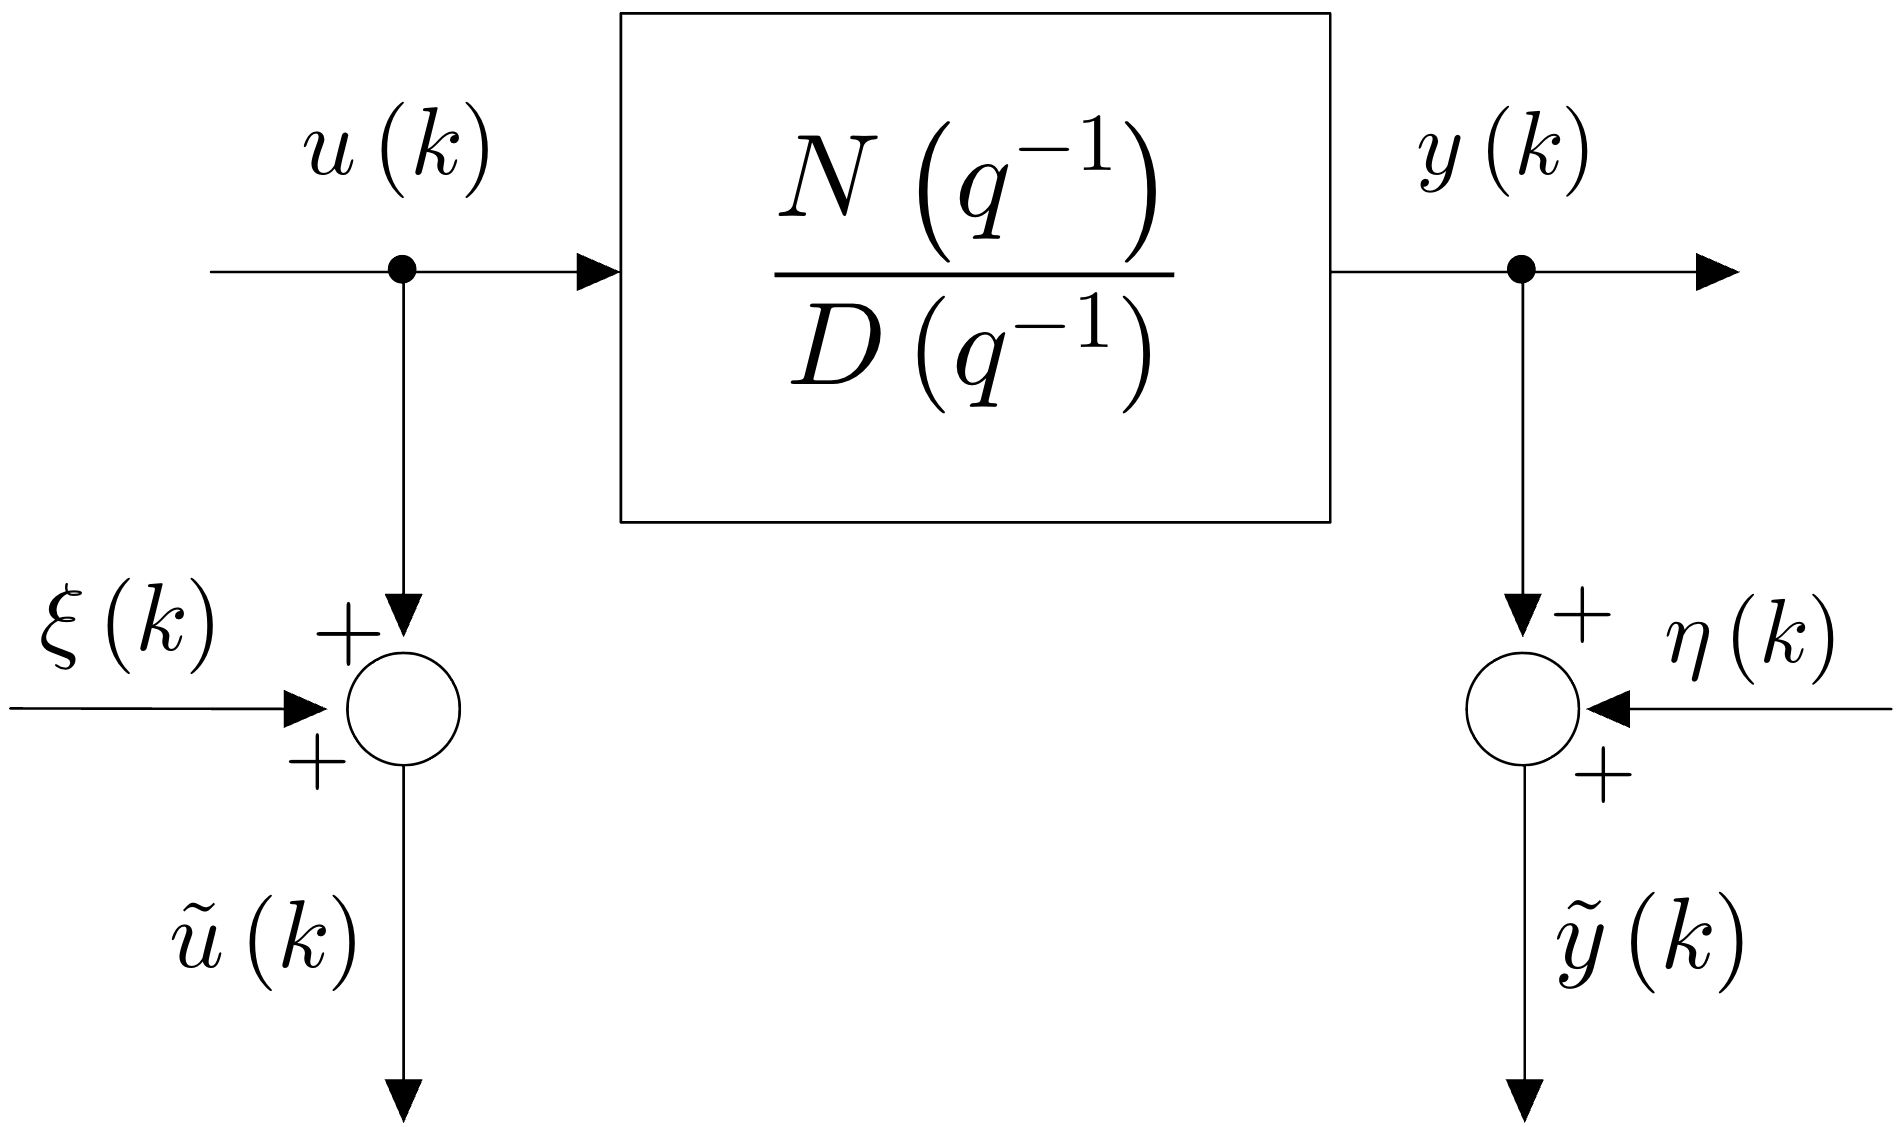
\includegraphics[scale=0.15]{img/EIV.jpeg}
    \caption{EIV SysId setting}
\end{figure}

\vspace{0.5cm}
\noindent
Once we have fixed the setting, the a-priori information to provide are about: 
\begin{itemize}
    \item The \textbf{model} for example $f\in\mathcal{F}$ where $\mathcal{F}$ is associated with a certain class of systems (eg. LTI, nonlinear, stable...)
    \item The \textbf{noise} and in particular information reguarding the \textbf{statistical distribution} (white, gaussian...) or the \textbf{boundedness} (depending on the approach we are going to follow).
\end{itemize}

\noindent
Now we are going to show an example which helps us to understand why the \textit{regression form} is an effective model for describing in the most general manner a dynamical system. 

\subsubsection{Example (Regression form for a second order LTI system)}
Let us consider a case in which we want to derive a model for a linear time-invariant system of the second order (a-priori assumption on the model: $f\in\mathcal{LTI}$, $n=2$), furthermore suppose there is no noise in the data. The regression form $y(u(k),\theta)$ is:
\begin{equation}\label{eq:reg_form}
    \begin{aligned}
        y(k)=-\theta_1{y(k-1)}-\theta_2{y(k-2)}+\theta_3{u(k)}+\theta_4{u(k-1)}+\theta_5{u(k-2)} 
    \end{aligned}
\end{equation}
It is useful now to remind an important property (\textbf{backward-shift operator}) that tells us $s(k-r)=q^{-r}s(k)$, for this reason the \ref{eq:reg_form} becomes:
\begin{align*}
    &y(k)=-\theta_1{q^{-1}} y(k) -\theta_2{q^{-2}}y(k)+\theta_3{u(k)}+\theta_4{q^{-1}}u(k)+\theta_5{q^{-2}}u(k) \iff\\
    &y(k)[1+\theta_1{q^{-1}}+\theta_2{q^{-2}}] = u(k) [\theta_3+\theta_4{q^{-1}}+\theta_5{q^{-2}}] \\
    & \frac{y(k)}{u(k)}=\frac{\theta_3+\theta_4{q^{-1}}+\theta_5{q^{-2}}}{1+\theta_1{q^{-1}}+\theta_2{q^{-2}}} \iff
    H(z) = \frac{\theta_3{z^2}+\theta_4{z}+\theta_5}{z^2+\theta_1{z}+\theta_2}
\end{align*}

\noindent
The last step comes up from the fact that can be dimostrated that it holds that $q^{-1}=z^{-1}$ and so from the regression form, passing through the backward-shift operator we can derive the transfer function of the system to be identified. Clearly a state-space description can be obtained once the parameters have been estimated by using the \textit{realization theory}  (transfer function $\to$ state space). \\

\noindent
This example shows us in an inductive way that the regression form is the right one to use!

\section{Least Squares estimation of the parameters $\theta_i$}
The objective of this paragraph is to show gradually -- using significative examples -- the problem of \textbf{parameter estimation} performed by using the \textbf{Least Squares (LS) model}, then we will analyze the pros and cons of such a method and some assumptions under which this kind of approach shows very nice properties (in a certain sense).

\subsection{Estimation of parameters in the noise-free case}
Let us consider again the case of a 2$^\text{nd}$ order LTI system; we have seen it is characterized by the following regression form: 
\begin{equation*}
    \begin{aligned}
        y(k)=-\theta_1{y(k-1)}-\theta_2{y(k-2)}+\theta_3{u(k)}+\theta_4{u(k-1)}+\theta_5{u(k-2)} 
    \end{aligned}
\end{equation*}
The objective of the SysId procedure is to estimate the parameter $\theta=[\theta_1, \theta_2, \theta_3,\theta_4, \theta_5]$. We have to carry out an \textbf{open-loop experiment} on the plant by injecting the sequence $u(k)$ and collecting the output $y(k)$ for $k=1,...,H$. Since in the regression form we use samples till $k-2$ we have to start from $n+1=3$. Then: 
\begin{equation}
    \begin{aligned} \label{eq:noise_free}
        &y(3)=-\theta_1{y(2)}    -\theta_2{y(1)} +\theta_3{u(3)} +\theta_4{u(2)}  +\theta_5{u(1)}\\
        &y(4)=-\theta_1{y(3)}    -\theta_2{y(2)} +\theta_3{u(4)} +\theta_4{u(3)}  +\theta_5{u(2)}\\
        &y(5)=-\theta_1{y(4)}    -\theta_2{y(3)} +\theta_3{u(5)} +\theta_4{u(4)}  +\theta_5{u(3)}\\
        &y(6)=-\theta_1{y(5)}    -\theta_2{y(4)} +\theta_3{u(6)} +\theta_4{u(5)}  +\theta_5{u(4)}\\
        &y(7)=-\theta_1{y(6)}    -\theta_2{y(5)} +\theta_3{u(7)} +\theta_4{u(6)}  +\theta_5{u(5)}
    \end{aligned}
\end{equation} 
In this case $H=3n+1=7$, it is quite evident we can express the equation \ref{eq:noise_free} in matrix form as:
\begin{equation}
    \underbrace{\begin{bmatrix}
        y(3)\\
        y(4)\\
        y(5)\\
        y(6)\\
        y(7)
    \end{bmatrix}}_{y} = \underbrace{\begin{bmatrix}
        -y(2)&-y(1)&u(3)&u(2)&u(1)\\
        -y(3)&-y(2)&u(4)&u(3)&u(2)\\
        -y(4)&-y(3)&u(5)&u(4)&u(3)\\
        -y(5)&-y(4)&u(6)&u(5)&u(4)\\
        -y(6)&-y(5)&u(7)&u(6)&u(5)\\
    \end{bmatrix}}_{A}\underbrace{\begin{bmatrix}
        \theta_1\\
        \theta_2\\
        \theta_3\\
        \theta_4\\
        \theta_5
    \end{bmatrix}}_{\theta}
\end{equation}
Then the five equations can be rewritten as $y=A\theta$, and in the case in which the matrix $A$ is invertible ($\det(A)\ne0$), the problem of estimating the $\theta$ parameters is simply:
\begin{equation}
    \theta=A^{-1}{y}
\end{equation}
The fact that must be $\det(A)\ne0$ is not so hard to guarantee since the first two columns of the matrix $A$ containing the samples of the output are likely to be very different! In order to prove it, it is sufficient to understand that for each LTI system there is a transient in which the output is not perfectly stabilized, even when the stimula assume very simple shapes (eg. step...). The matrix $A$ is square by construction, then since we have $h=2n+1=5$ parameters, we need 5 equations to obtain a unique solution to the problem. This approach is valid even with nonlinear functions which \textit{depends linearly on the parameters}, we are sampling input and output, for this reason it is not important that the function $f$ (of the regression form) is nonlinear. Important remarks: 
\begin{itemize}
    \item For a system of order $n$ we need to estimate $h=2n+1$ parameters; 
    \item The minimal number of samples we need is $H=3n+1$
    \item We can start applying the regression form function from the instant $k=n+1$, since it depends on both preceeding output and input.
\end{itemize}

\subsection{Estimation of parameters in the noisy case}
The fact that the collected samples were noisy free was only a simplificative assumption made up to introduce the problem. In real-world applications there is always uncertainty. Let us consider an example which will make necessary the collection of more and more data.\\
Let us consider a static system of the type\footnote{
    This could be for example a model for a resistor in which flows a certain current ($u(k)$) and we want to measure the voltage ($y(k)$).}
\begin{equation}
    y(k)=\theta{u(k)}
\end{equation}
It seems that we can correctly estimate $\theta$ by just collecting a \textit{simple pair} $(u(k),y(k))$ in order to obtain $\theta=\frac{y(1)}{u(1)}$. Now let us assume that the input data are exact, while the output sample $y(1)$ is corrupted by a noise $\eta(1)$. What is obtained is as follows:
\begin{equation*}
    \begin{cases}
        \tilde{u}(k)=u(k)\\
        \tilde{y}(k)=y(k)+\eta(k)
    \end{cases}
\end{equation*}
Since $\tilde{y(k)}\ne{y(k)}$, the estimate given by $\frac{y(1)}{u(1)}$ is completely wrong, since:
\begin{equation*}
    \hat{\theta}=\frac{\tilde{y}(1)}{u(1)}=\frac{y(1)+\eta(1)}{u(1)}=\theta+\frac{\eta(1)}{u(1)}\ne\theta
\end{equation*}
\textbf{What to do?} The idea is to collect a number of data $H\gg{2n+1}$, in this case the matrix $A$ becomes a tall matrix, there is not a unique solution as in the case of the noise-free example, but we can get an approximation $\hat{\theta}$ such that $\tilde{y}\thickapprox{y}$. The following steps can be done:
\begin{equation}\label{eq:normal__equations} \tag{\textsf{Normal Equations}}
    \tilde{y}={A}\theta \to A^T{\tilde{y}} = (A^T{A})\theta \iff \theta=\underbrace{(A^T{A})^{-1}A^T}_{A^*}{\tilde{y}}
\end{equation}
where $A^*$ is the Moore-Penrose pseudoinverse (generalization of the inverse for non-square matrices)\footnote{
    Keep in mind it is derived from the Singular Value Decomposition (SVD), which the generalization of the spectral Decomposition for non-symmetric matrices.
}. It can be demonstrated\footnote{
    The problem (\ref{eq:LS}) appears to be a convex quadratic unconstrained minimization problem. If the functional is explicitly written as a quadratic function, then after computing the gradient, its root raises the normal equations.
} that the (\ref{eq:normal__equations}) is the solution of the problem:
\begin{equation} \label{eq:LS} \tag{\textsf{LS}}
    \theta_{LS}=\arg\min_{\theta} \Vert \tilde{y}-A\theta \Vert_2^2
\end{equation}
that is the well-known \textbf{Least-Squares problem}. This is a statistical approach to \textit{parameter estimation} which has nice properties:
\begin{itemize}
    \item The \textit{computational burden} is very low! The only needed operation is the inversion of $A^T{A}$;
    \item There is a recursive way to solve it that reduces the work load in presence of big matrices (online computation).\footnote{
        See for more details: \url{https://en.wikipedia.org/wiki/Recursive_least_squares_filter}%{Recursive Least Squares filtering (wikipedia(en))}
    }
    \item The most important and 'powerful' property is the \textbf{consistency property}, which holds when two assumptions are satisfied. The next paragraph deals with the explanation of such assumptions.
\end{itemize}

\subsection{Least Squares: consistency property}
\begin{theorem}[\textsf{Consistency Theorem}] If the following two assumptions are satisfied:
\begin{enumerate}
    \item The noise can be considered as an additive term entering the problem that is
    \begin{align*}
        y(k) = &-\theta_1{y(k-1)}-\theta_2{y(k-2)}-...-\theta_n{y(k-n)}\\
        &+\theta_{n+1}u(k)+\theta_{n+2}u(k-1)+...+\theta_{n+m+1}u(k-m) + \underbrace{e(k)}_{\textsf{EQUATION ERROR}}
    \end{align*}
    \item The samples $e(k)$, $k=1,...,H$ are indipendent and identically distributed (white) random variables which can be modeled through a \textbf{zero-mean Gaussian noise}
\end{enumerate}
Then, it holds that\footnote{
    We take the expected value of the estimate since random variables are introduced in the problem by adding $e(k)$, the estimate itself becomes a random variable.
}:
\begin{equation}\label{eq:consistency}
    \lim_{H\to\infty} \mathbb{E}[\theta_{LS}] = \theta
\end{equation}
\end{theorem}
In a simplified way such a theorem states that under the two assumptions (satisfied), if you enlarge $H$, $\theta_{LS}\to\theta$.

\subsection{Analysis of the assumptions}
At this point, we wonder if the just exposed result, solved all of our problem for the parameter estimation, and then if the LS approach can be used in general. This is nothing but verifying if the two hypotesis are satisfied. For the sake of clarity let us take the most general setting for an experiment on a plant to identify (EIV).\\
Grasping on the a-priori information that the system is an LTI second-order one, let us take the associated regression form
\begin{equation*}
    \begin{aligned}
        y(k)=-\theta_1{y(k-1)}-\theta_2{y(k-2)}+\theta_3{u(k)}+\theta_4{u(k-1)}+\theta_5{u(k-2)} 
    \end{aligned}
\end{equation*}
Since $u(k)=\tilde{u}(k)-\eta(k)$ and ${y}(k)=\tilde{y}(k)-\xi(k)$, we can substitute them obtaining:
\begin{equation}
    \begin{aligned} \label{eq:ee_equation}
    \tilde{y}(k)=&-\theta_1{\tilde{y}(k-1)}-\theta_2{\tilde{y}(k-2)}+\theta_3{\tilde{u}(k)}+\theta_4{\tilde{u}(k-1)}+\theta_5{\tilde{u}(k-2)}+\\
    &\underbrace{+\theta_1{\eta(k-1)}+\theta_2{\eta(k-2)}-\theta_3{\xi(k)}-\theta_4{\xi(k-1)}-\theta_5{\xi(k-2)}}_{e(k)}
\end{aligned}
\end{equation}
It is evident, I can envelope all the terms associated with the noise samples in a term which I call $e(k)$. Then, \textbf{the first assumption is satisfied}. What about the second? We have to check if the sequence 
\begin{equation}\label{eq:EquationError} \tag{\textsf{EE}}
    {e(k)}=\theta_1{\eta(k-1)}+\theta_2{\eta(k-2)}-\theta_3{\xi(k)}-\theta_4{\xi(k-1)}-\theta_5{\xi(k-2)}
\end{equation}
is a white one (samples iid). Let us analyze a pair of samples:
\begin{align*}
    e(3)=\theta_1{\color{red}\eta(2)}+\theta_2\eta(1)-\theta_3{\color{red}\xi(3)}-\theta_4{\color{red}\xi(2)} -\theta_5\xi(1)\\
    e(4)=\theta_1{\eta(3)}+\theta_2{\color{red}\eta(2)}-\theta_3\xi(4)-\theta_4{\color{red}\xi(3)} -\theta_5{\color{red}\xi(2)}\\
\end{align*}
How it is highlighted, only by taking two of the $e(k)$ we can note they depend from common samples, for this reason the sequence $e(k)$ itself it is not white at all! They will provide an estimate $\theta_{LS}$ which is not going to enjoy of the consistency property. Even if the setting was OE instead of EIV, the same conclusion would have been drawn.

\section{The Equation Error (EE) noise structure}
We have concluded in the former paragraph that the LS estimate is not suitable in the case we have either an EIV or an OE setting. Thus, what is the case in which the LS can be used? (again: that is, the two assumptions are verified). It is necessary to better dissect the properties of (\ref{eq:ee_equation}). In particular, it is useful (passing through the backward-shift operator) finding what is the relation between $\tilde{y}(k)$, $u(k)$ and $e(k)$. In order to discover such properties let us assume that the setting used is the Output Error (without loss of generality). Using $s(k-r)=q^{-r}s(k)$ we can write: 
\begin{align}
    &\tilde{y}(k) [1+\theta_1{q^{-1}}+...+\theta_n{q^{-n}}]= u(k) [\theta_{n+1}+\theta_{n+2}q^{-1}+...+\theta_{n+m+1}q^{-m}]+e(k) \iff\\
    &\tilde{y}(k) = \frac{[\theta_{n+1}+\theta_{n+2}q^{-1}+...+\theta_{n+m+1}q^{-m}]}{[1+\theta_1{q^{-1}}+...+\theta_n{q^{-n}}]} u(k) + \frac{1}{[1+\theta_1{q^{-1}}+...+\theta_n{q^{-n}}]}e(k) = \\
    &=\frac{N(q^{-1})}{D(q^{-1})} u(k)+\frac{1}{D(q^{-1})}e(k)=\frac{N(z)}{D(z)} u(k)+\frac{1}{D(z)}e(k)
\end{align}
The deriving setting is represented in the figure below:
\begin{figure}[h]
    \centering
    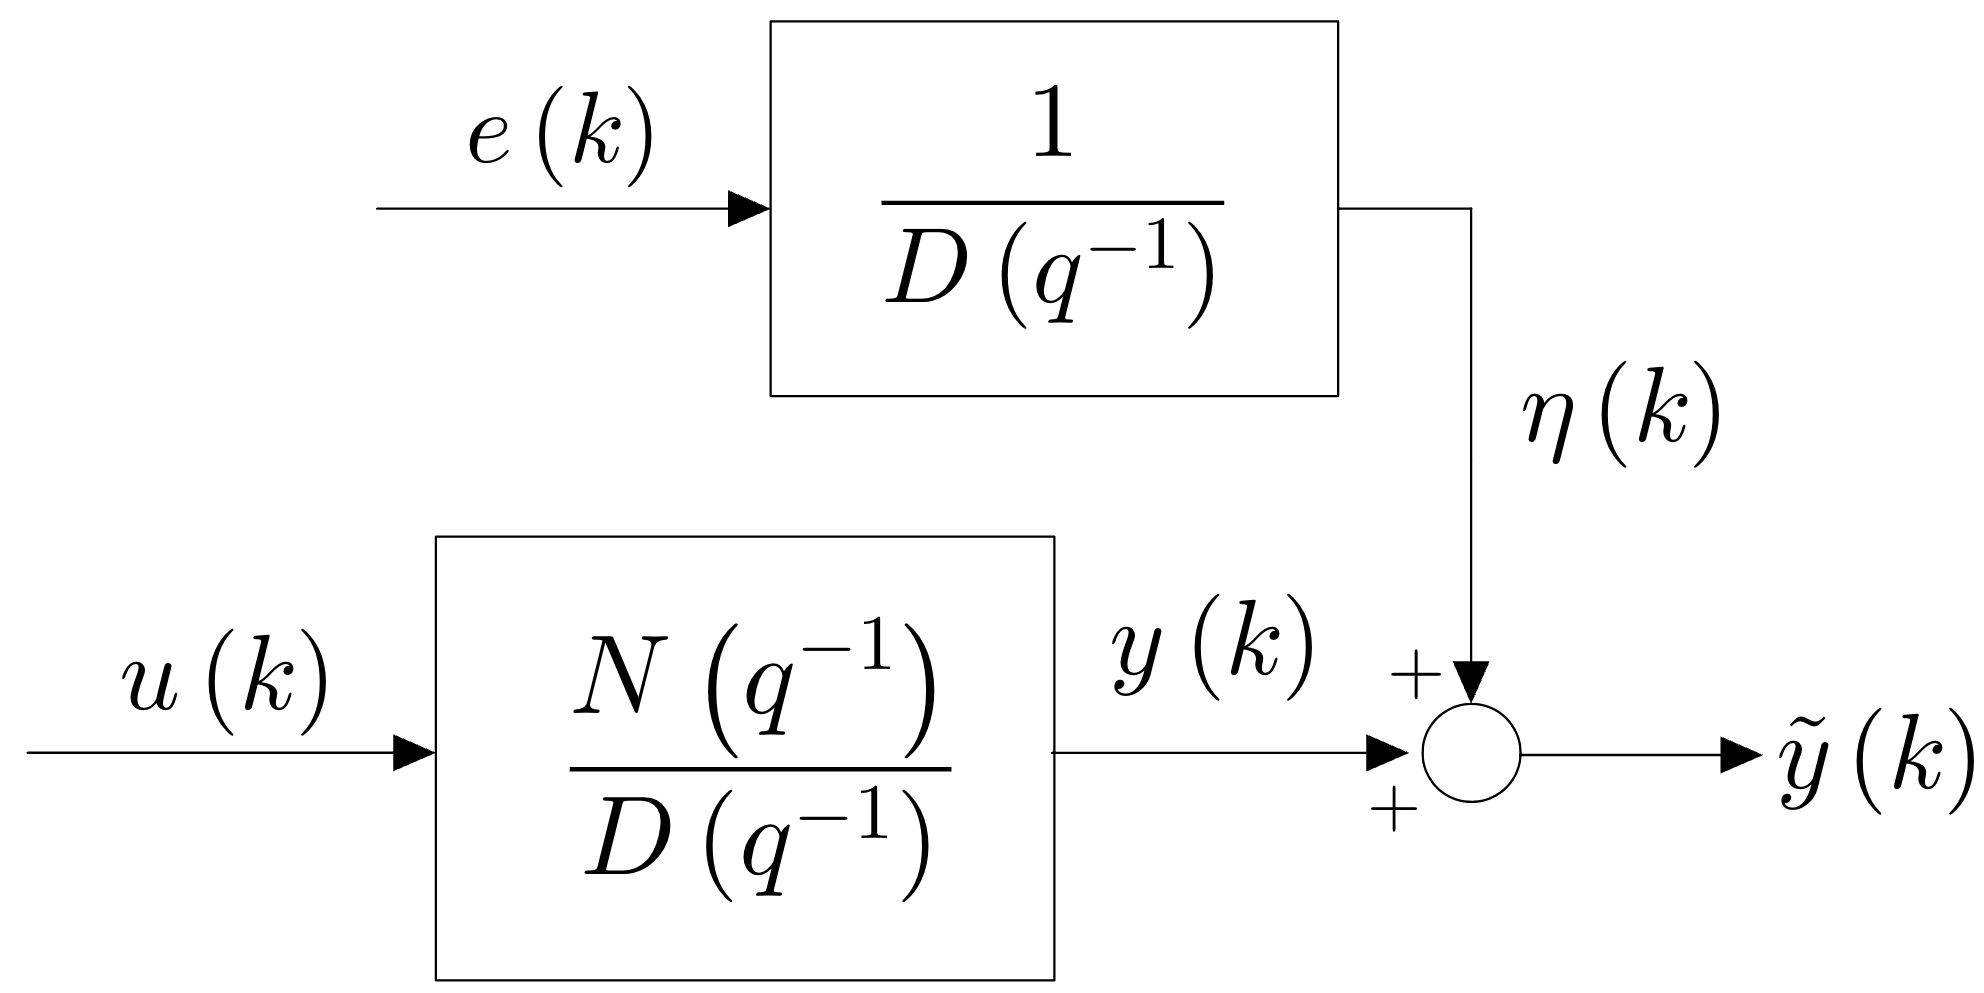
\includegraphics[scale=0.15]{img/EE.jpeg}
    \caption{Equation Error (EE) noise structure}
\end{figure}

\noindent
In this way we can conclude that the LS estimate makes sense if the date corrupted by a random sequence $e(k)$ (the noise) filtered by a system whose transfer function is the denominator of the system to be identified! No sense, since the sensor in general has nothing to share with the plant we want to identify. 
However there are some cases in which the LS approach can be used, we refer to the few cases in which the plant to be identified is such that $D(q^{-1})=1$. This occurs when I have to do:
\begin{itemize}
    \itemsep-0.2em
    \item Identification of \textbf{FIR systems} (Finite impulse response); 
    \item Identification of static systems;
\end{itemize}
\noindent
When the denominator of the transfer function is equal to one, the Equation Error plays the role of the \textit{output measurement error} $\eta(k)$. In this case also the \textbf{second assumption} is satisfied.


\subsection{System Identification of Finite Impulse Response (FIR) systems}
This of type of system has a transfer function which depends only on the samples of the input and not on on the previous output samples.

\begin{equation}
    \tilde{y}(k)=\theta_1{u(k)}+\theta_2{u(k-1)}+...+\theta_n{u(k-n)}+
    \underbrace{e(k)}_{\eta(k)}
\end{equation}
Here also the second assumption is satisfied since the error samples are iid. In the case of FIR the property (\ref{eq:consistency}) is fulfilled.

\subsection{System Identification of Static systems}
Here the output is a function of parameters $\theta_i$ and of the input $u(k)$ at the current instant.
\begin{equation}
    y(k)=\theta_1{g_1({u(k)})} + 
    \theta_2{g_2({u(k)})} + ... +
    \theta_n{g_n({u(k)})} + e(k)
\end{equation}
The functions $g_i(u(k))$ can be trigonometric functions, polynomial or anyway any other basic function.

\section{Final remarks}
Real experimets have data characterized by noise and in general the consistency property does not hold, in some situations in which the problem has a particular structure the assumptions required are perfectly fulfilled. We have understood that the most critical problem to manage is the second assumption which require the error to be white, zero mean and Gaussian (very strong assumptions!), moreover the resulting noise structure reaches a quite strange conclusion in which it is required that the system and the sensor share a part of their model. \\
In the following we will see another approach that, differently from LS, replaces the Assumption (2) with something that is significantly \textit{less strong}.

\chapter[Set-Membership Identification: intro, Equation-Error]{Set-Membership Identification: an introduction, Equation-Error noise structure}

The objective of this chapter is to introduce an approach for the parameter estimation which requires to do less strong assumption on the noise affecting the experimentally collected data. After a brief introduction with the crucial ingredients, we will go on with some instructive examples which will bring us to the complete formulation of the \textbf{Set-Membership System Identification procedure}.

\section{Ingredients for Set-Membership System Identification}
As usual in order to perform correctly the procedure of System Identification we need some crucial ingredients:
\begin{itemize}
    \itemsep-0.2em
    \item[\ding{182}] \textbf{\textsf{A-priori assumption on the system:}}
    \begin{enumerate}
        \item[\ding{51}] We use the general \textbf{regression form} 
        \begin{equation} 
            y(k)=f(y(k-1), y(k-2),  ..., y(k-n), u(k-1), ..., u(k-m), \theta)
        \end{equation}
        \item[\ding{51}] The \textbf{class of function} $\mathcal{F}$ and the order of the system $n$;     
    \end{enumerate}
   
    \item[\ding{184}] \textbf{\textsf{A-priori information of the noise}} and in particular:
    \begin{enumerate}  
        \itemsep-0.2em
        \item[\ding{51}] \textbf{Noise structure}: is referred to the way the uncertainty enters  into the problem.
        \item[\ding{51}] \textbf{Characteristic of the signal}, it is remarkable that here we assume something different and weaker. We will assume that the noise sequence/sequences (depending on the noise structure) belongs to a certain bounded set $\mathcal{B}$.
    \end{enumerate}
\end{itemize}

\section{Set-Membership Identification of LTI system with EE noise structure}
In this paragraph we will show what is obtained in term of parameter estimation, when we have that the a-priori information on the noise are the following:
\begin{itemize}
    \itemsep-0.3em
    \item[\ding{51}] The uncertainty enter in the problem as an additive term which we call $e(k)$ (the same of the first assumption of the theorem), that is:
    \begin{align*}
        y(k) = &-\theta_1{y(k-1)}-\theta_2{y(k-2)}-...-\theta_n{y(k-n)}\\
        &+\theta_{n+1}u(k)+\theta_{n+2}u(k-1)+...+\theta_{n+m+1}u(k-m) + \underbrace{e(k)}_{\textsf{EQUATION ERROR}}
    \end{align*}
    \item[\ding{51}] We suppose on the sequence characterizing the error is \textbf{bounded} (this is the crucial difference with respect to what requires the \textit{consistency theorem}), that is:
    \begin{equation}\label{eq:boundedness}
        e(k)\in\mathcal{B}_e \iff \vert e(k) \vert \le \Delta_e, \ k=1, ..., H
    \end{equation}
\end{itemize}
\subsection{Feasible Parameter Set $\mathcal{D}_\theta$}

\begin{quotation}
    \noindent
    \textsf{In this paragraph by using some examples, we will define the \textit{feasible parameter set} and its fundamental properties, in particular, it is useful to derive a \textbf{mathematical formulation of such a set} in order to explore its \textit{usefulness} and \textit{boundedness}}
\end{quotation}

\noindent
The set of solutions for the identification problem is implicitly described on what is called the \textbf{Feasible Parameter Set (FPS)}, we will indicate it with $\mathcal{D}_\theta$.

\begin{definition}[\textsf{\textbf{FEASIBLE PARAMETER SET}}] \textit{The \textbf{Feasible Parameter Set} $\mathcal{D}_\theta$ is the set of all the values of the parameter $\theta=[\theta_1 ... \theta_n]^T$ which are consistent (coherent) with all the available a-priori information (system and noise) and all the collected data (a-posteriori information).}
\end{definition}


\noindent
In order to better understand the meaning of $\mathcal{D}_\theta$ let us assume we are collecting data in the OE setup, and we know that $\vert \eta(k) \vert \le \Delta_\eta$. The input sequence, then, is perfectly known while the output is corrupted by the noise $\eta(k)$.

\begin{figure}[h]
    \centering
    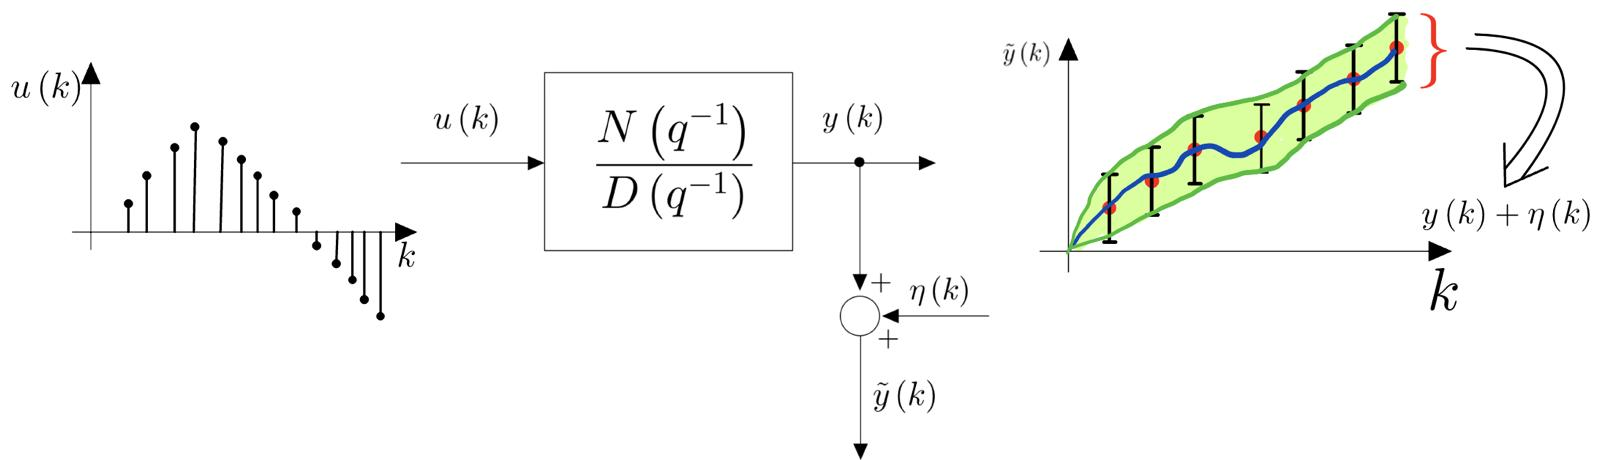
\includegraphics[scale=0.32]{img/oe_example.jpeg}
    \caption{OE set-up experiment}
\end{figure}

\noindent
The question is: \textsf{Is the SM approach providing us a pointwise estimate for the parameter $\theta$?} We will show more or less formally in the following that the answer is NO, but we can track an intuitive reasoning which will bring us to the same conclusion. \\
For this aim, given the sequence $u(k)$, we collect an output $\tilde{y}(k), \ k=0, 1, ...$. Moreover, let us suppose that for such collected data the obtained model is giving us some parameter $\theta$ such that the I/O mapping is the one indicated with the {\color{blue} blue} line. Now, since the output measurements are affected by noise, all of the samples between $[\tilde{y}(k)-\eta(k), \tilde{y}(k)+\eta(k)]$\footnote{
    See the black vertical bars
} is providing us an information which is coherent with the a-priori assumption on the noise itself. Besides, another couple of parameter $\theta_1, \theta_2$ derived from such samples, can be also the result of our identification problem. From the reasoning we have just presented we can intuitively understand that:
\begin{quotation} 
    \noindent
    \textsf{probably the parameter $\theta_i$ are provided with an \textbf{uncertainty interval} since also the experimental data are provided with uncertainty.}
\end{quotation}

\subsection{Mathematical formulation of the FPS}
We know that the system is a \textbf{second order}, \textbf{LTI one} (\textit{a-priori assumption on the system}), the uncertainty/noise enters the identification problem as additive term $e(k)$ (equation error) and it is \textbf{bounded} (that is $\vert e(k)\vert \le \Delta_e, \ k=0,1, ..., H$) (\textit{a-priori assumption on the noise}), after having collected the data $\tilde{y}(k)$, after having stimulated the system to be identified with a sequence $\tilde{u}(k)$ (\textit{a-posteriori information})\footnote{
    An EIV(Errors-in-variables) set-up is assumed, then, in order to be more precise the input is given by a subsystem, this is the reason why we have to measure it.
}, we can define the \textsf{Feasible Parameter Set} as follows:

\begin{equation} \label{eq:FPS_2nd}
    \begin{aligned}
        \mathcal{D}_\theta=&\{\theta\in\mathbb{R}^p: \ 
                \tilde{y}(k)=-\theta_1\tilde{y}(k-1)
                -\theta_2\tilde{y}(k-2)+\\
                &+\theta_3\tilde{u}(k)
                +\theta_4\tilde{u}(k-1)
                +\theta_5\tilde{u}(k-2)+e(k), \quad k=3,...,H\\
                &  \vert e(k) \vert \le \Delta_e, \quad k=1,...,H
        \}
    \end{aligned}
\end{equation}
The set (\ref{eq:FPS_2nd}) is made up of both inequality and equality constraints, moreover it appears clear that it is a \textit{subset of $\mathbb{R}^p$} with $p$ the number of parameters. There is a problem: the set $\mathcal{D}_\theta$ is defined using some inequality constraints on the noise samples $e(k)$ which are not part of the parameter space. In the following a way to eliminate such a dependence is shown, without adding any approximation or conservativeness.

\begin{equation*} 
    \begin{aligned}
        \mathcal{D}_\theta=&\{\theta\in\mathbb{R}^p: \ 
                \tilde{y}(k)+\theta_1\tilde{y}(k-1)
                +\theta_2\tilde{y}(k-2)+\\
                &-\theta_3\tilde{u}(k)
                -\theta_4\tilde{u}(k-1)
                -\theta_5\tilde{u}(k-2)=e(k), \quad k=3,...,H\\
                &  \vert e(k) \vert \le \Delta_e, \quad k=1,...,H
        \}= \\
        &\{\theta\in\mathbb{R}^p: \ 
                \vert \tilde{y}(k)+\theta_1\tilde{y}(k-1)
                +\theta_2\tilde{y}(k-2)+\\
                &-\theta_3\tilde{u}(k)
                -\theta_4\tilde{u}(k-1)
                -\theta_5\tilde{u}(k-2) \vert \le \Delta_e, \quad k=3,...,H
        \}
    \end{aligned}
\end{equation*}
In this way, we have obtained an implicit description of the \textbf{set of all the feasible solution of our identification problem} in term of a \textit{set of inequality contraints only involving $\theta$}.\\


\begin{multicols}{2}
    \noindent
    A graphical representation of such a set in a 2-dimensional parameter space is shown in the figure on the side. Here the objective is to analyze two main features of the Feasible Parameter Set by formulating the following two questions:  
    \normalsize{
    \begin{itemize}
        \itemsep-0.2em
        \item[(Q1)] \textsf{\textbf{\color{red}Boundedness}} Is this set a bounded one? Under which conditions?
        \item[(Q2)] \textsf{\textbf{\color{red}Usefulness}} What is the relation between $\mathcal{D}_\theta$ and $\theta_{\text{true}}$?
    \end{itemize}}
    \newcolumn
    \begin{center}
        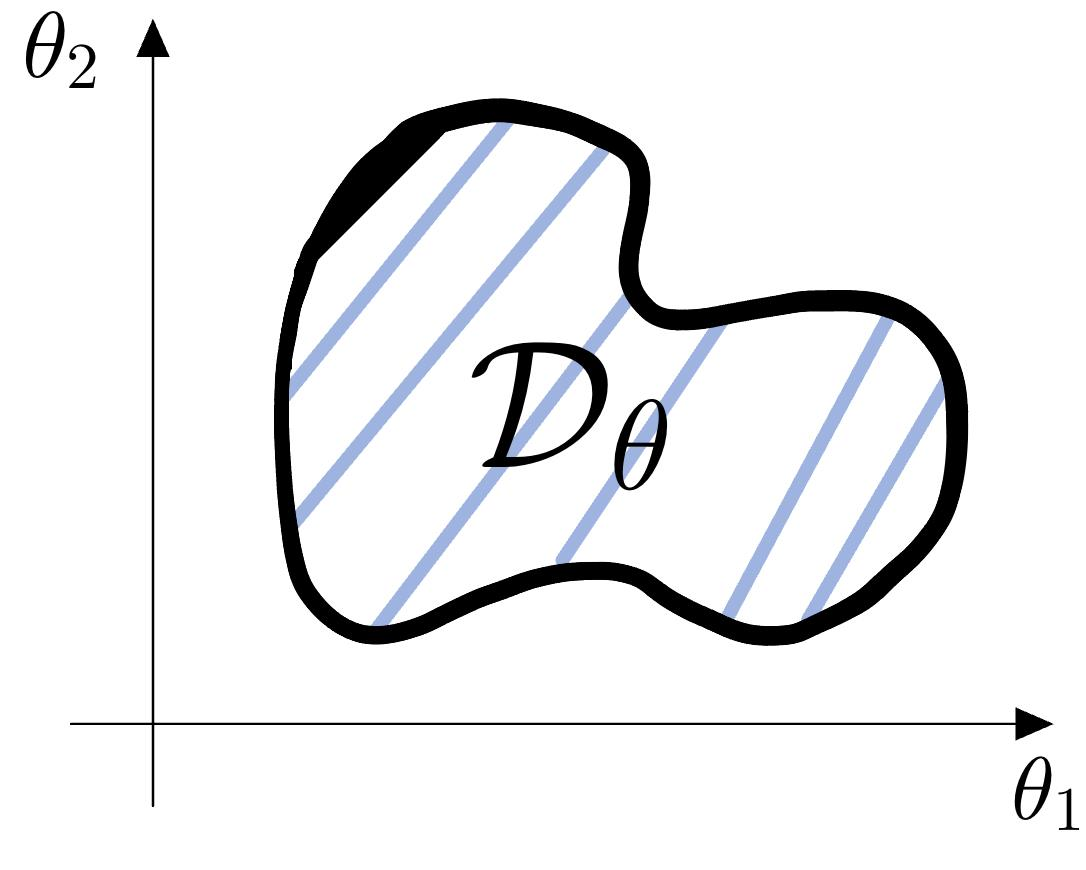
\includegraphics[scale=0.18]{img/FPS_1.jpeg}
    \end{center}
\end{multicols}
\subsubsection{Main features of $\mathcal{D}_\theta$}


\noindent
\textsf{\underline{Question Q1}} The boundedness of $\mathcal{D}_\theta$ depends on the way we collect the data (in general) ($\Rightarrow$ this concept has to be better specified in the next slides). \textit{For the moment let us assume that such a set is bounded}.\\

\noindent
\textsf{\underline{Question Q2}} Assuming that the a-priori assumptions on the system and on the noise are correct, then $\theta_{\text{true}}$ is guaranteed to belong to $\mathcal{D}_\theta$ (this is very important for further theory development).\\

\noindent
Once that we have obtained an implicit description of $\mathcal{D}_\theta$, \textit{how can we extract a useful model from it,either for simulating the system or designing a feedback controller for such a system?} Before saying it, we have to  distinguish \textit{two different classes} of SM estimation algotrithms: 
\begin{itemize}
    \itemsep-0.2em
    \item[(E1)] \textsf{\textbf{\color{red} Set-valued estimators}}, defined as estimation algorithms which provides a (possibly) conservative estimate of $\mathcal{D}_\theta$ in a \textbf{simplified geometrical form} that can be easily used to simulate or control the system; 
    \item[(E2)] \textsf{\textbf{\color{red} Pointwise Estimators}}, defined as estimation algorithms that provides a single value of $\theta$ which is an optimal estimate of $\theta_{\text{true}}$ in some sense.
\end{itemize}
Here, among all the possible estimator in the class (E1), we consider the algorithm which is providing the \textbf{minimum volume box outerbounding $\mathcal{D}_\theta$}. Such an estimator is implicitly providing what we will call \textbf{Parameter uncertainty Intervals (PUIs)}. 

\begin{multicols}{2}
    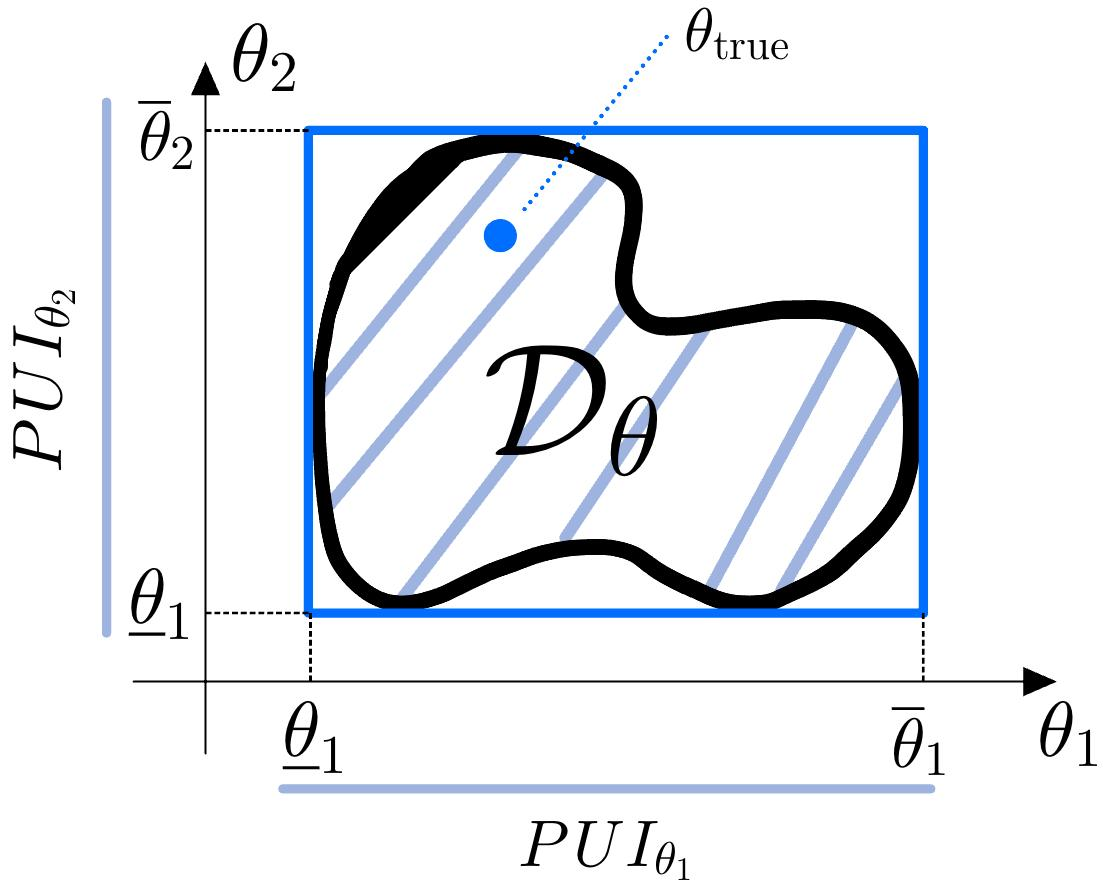
\includegraphics[scale=0.2]{img/PUI_1.jpeg}
    The PUI are defined as follows:
    \newcolumn
    \begin{equation}
        PUI_{\theta_j} = [\underline{\theta}_j,
        \overline{\theta}_j]
    \end{equation}
    where the extrema of the interval are:
    \begin{align}
        &\underline{\theta}_j \doteq \min_{\theta\in\mathcal{D}_\theta} {\theta_j}\\
        &\overline{\theta}_j \doteq \max_{\theta\in\mathcal{D}_\theta} {\theta_j} = \min_{\theta\in\mathcal{D}_\theta}{-\theta_j}
    \end{align}
    It is remarkable that each $PUI$ is providing the \textbf{minimum uncertainty interval} for each parameter $\theta_j$. In the figure are shown the $PUI$ for the feasible parameter set presented before.
\end{multicols}
\noindent 
Note the that, in the case of $\mathcal{D}_\theta \subseteq \mathbb{R}^2$ the minimum volume containing $\mathcal{D}_\theta$ is a rectangular shape whose sides are the parameter uncertainty intervals associated to $\theta_1$ and $\theta_2$.

\subsubsection{\color{orange}Usefulness of the PUIs}
Suppose you have for the following model, the corrensponding PUIs:
\begin{equation*}
    G(z)=\frac{\theta_2}{z+\theta_1} \quad
    \theta_2 \in [\underline{\theta}_2, \ \overline{\theta}_2] = PUI_{\theta_2}, \quad
    \theta_1 \in [\underline{\theta}_1, \ \overline{\theta}_1] = PUI_{\theta_1}
\end{equation*}
Moreover, you assume you want to derive a Lead/Lag controller for such a system. It is well known that the main idea behind this approach is having a representation of the loop function $L(s)$, and adding a certain number of dynamic networks in order to change the shape of $L(s)$ itself, in order to obtain a certain $\omega_{c, des}$ In this framework, we have not a single loop function but a cloud of them, from which we can retrieve a bound of  some type in order to derive a controller in the \textbf{limit cases}.

\begin{figure}[h]
    \centering
    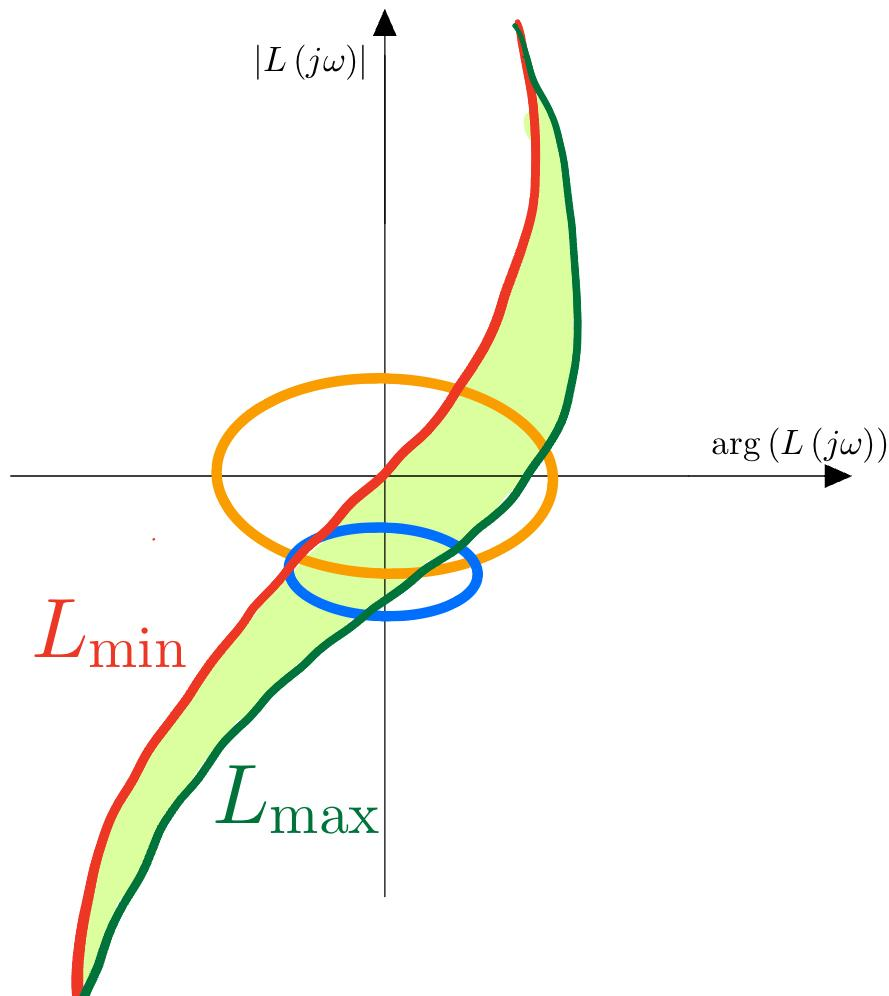
\includegraphics[scale=0.2]{img/Nichols.jpeg}
    \caption{Nichols plot of the loop function}
\end{figure}
At this aim, the following figure for example shows the \textit{frequency response} on the Nichols' Plot of the loop function. According to the choice of the parameters one can obtain a different plot in the range of curves delimited by $[L_{min}, L_{max}]$.

\subsection{Geometric shape of the Feasible Parameter Set}
In the case we have a linear time-invariant system where the uncertainty can be described by means of an unknown but bounded \textit{equation error} $e(k)$, we can obtain a particular shape of the FPS which makes the problem particularly 'simple' to solve. \\
For sake of simplicity, the description of such a property by using a first order system ($n=1$) is done. At this aim, we know that the transfer function has the shape:
\begin{equation}
    G(z)=\frac{\theta_2{z}}{z+\theta_1} \longrightarrow
    G({q^{-1}}) = \frac{\theta_2}{1+\theta_1{q^{-1}}}=\frac{y(k)}{u(k)}
\end{equation}
From which you can find that the regression form is:
\begin{equation}
    y(k)+\theta_1{y(k-1)}=\theta_2{u(k)} \iff 
    y(k) = -\theta_1{y(k-1)}+\theta_2{u(k)}
\end{equation}
This result has been issued by using the \textbf{a-priori information on the system}: LTI and $n=2$. On the other hand, we know that the noise enters the equation as an \textit{unknown but bounded} equation error $e(k)$, that is
\begin{equation*}
    \vert e(k) \vert \le \Delta_e   \quad k=1,..., N
\end{equation*}
Finally, the \textbf{a-posteriori information} are the experimentally collected data, which both are corrupted by measurement noise. 
\begin{equation*}
    \tilde{u}(k)=u(k)+\xi(k), \quad 
    \tilde{y}(k)=y(k)+\eta(k) \quad \forall k=1, ..., N
\end{equation*}
Putting all together, we can find the implicit mathematical formulation of the FPS as follows:

\begin{equation}
    \begin{aligned}
        \mathcal{D}_\theta = &\{
            \theta\in\mathbb{R}^2: \ 
            \tilde{y}(k)=-\theta_1\tilde{y}(k-1)+\theta_2{\tilde{u}(k)} + e(k), \quad k=2, ..., N, \\
            & \vert e(k) \vert \le \Delta_e   \quad k=1,..., N
        \}=\\
        &=\{\theta\in\mathbb{R}^2: \
            \vert
            \tilde{y}(k)+\theta_1\tilde{y}(k-1)-\theta_2{\tilde{u}(k)}
            \vert  \le \Delta_e, \quad k=2,..., N
        \}=\\
        &=\{ \theta\in\mathbb{R}^2: \ -\Delta_e \le 
            \tilde{y}(k)+\theta_1\tilde{y}(k-1)-\theta_2{\tilde{u}(k)}
            \le \Delta_e, \quad k=2,...,N
        \}=\\
        &=\{\theta\in\mathbb{R}^2: \
            {\color{red}\theta_1\tilde{y}(k)-\theta_2\tilde{u}(k) \le \Delta_e-\tilde{y}(k)} \quad \textsf{(C1)} \\
            &\qquad \qquad \quad{\color{blue}-\theta_1\tilde{y}(k)+\theta_2\tilde{u}(k) \le \Delta_e+\tilde{y}(k)} \quad \textsf{(C2)}, \quad k=2, ..., N
        \}
    \end{aligned}
\end{equation}
\noindent
For each $k$, from $\mathcal{D}_\theta$ we obtain a couple of straight lines. Let us represent them by computing the constraints $\textsf{(C1)}$ and $\textsf{(C2)}$ for $k=2,3$

\subsubsection{Constraints for \color{red} $k=2$}
\begin{align}
    \tag{\color{red}\textsf{C1}}
    &\begin{aligned}\label{eq:c1_1}
        &\tilde{y}(2)+\theta_1{\tilde{y}(1)}-\theta_2\tilde{u}(2) \le \Delta_e \\
        &\theta_2 \ge \frac{\tilde{y}(1)}{\tilde{u}(2)}\theta_1 + \frac{\tilde{y}(2)-\Delta_e}{\tilde{u}(2)}
    \end{aligned}\\
    \tag{\color{blue}\textsf{C2}}
    &\begin{aligned}\label{eq:c1_1}
        &\tilde{y}(2)+\theta_1{\tilde{y}(1)}+\theta_2\tilde{u}(2) \le -\Delta_e \\
        &\theta_2 \le \frac{\tilde{y}(1)}{\tilde{u}(2)}\theta_1 + \frac{\tilde{y}(2)+\Delta_e}{\tilde{u}(2)}
    \end{aligned}
\end{align}
We can note that such lines have the \textbf{same angular coefficient} but different \textbf{intercept}. Roughly speaking they are parallel straight lines, that in form of inequalities define some \textit{halfplanes}. Since in the FPS the constraints must be satisfied \textbf{for each $k$}, we take the intersection of such constraints. In the specific case they result in a \textbf{strip}. Such a set is unbounded, this is related to the fact we used a single constraints against two degree of freedom (that is 2 parameters). 

\begin{figure}[h]
    \centering
    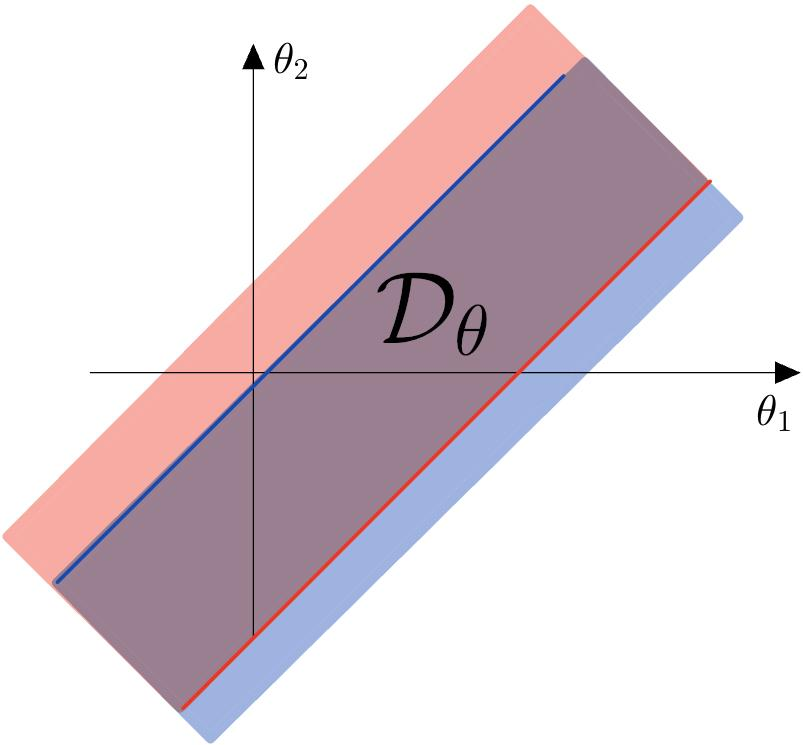
\includegraphics[scale=0.22]{img/strip.jpeg}
    \caption{$\mathcal{D}_\theta$ resulting from a single equation}
\end{figure}
\noindent
A possible representation is given in the figure above. Now, in order to obtain a bounded set we must collect $k=3$ data while using at least 2 equations resulting in 2 pairs of constraints $\textsf{C1-C2}$.
\subsubsection{Constraints for \color{red} $k=3$}
Following the same reasoning we obtain:
\begin{align}
    \tag{\color{red}\textsf{C1}}
    &\begin{aligned}\label{eq:c1_1}
        &\tilde{y}(3)+\theta_1{\tilde{y}(2)}-\theta_2\tilde{u}(3) \le \Delta_e \\
        &\theta_2 \ge \frac{\tilde{y}(2)}{\tilde{u}(3)}\theta_1 + \frac{\tilde{y}(3)-\Delta_e}{\tilde{u}(3)}
    \end{aligned}\\
    \tag{\color{blue}\textsf{C2}}
    &\begin{aligned}\label{eq:c1_1}
        &\tilde{y}(3)+\theta_1{\tilde{y}(2)}+\theta_2\tilde{u}(3) \le -\Delta_e \\
        &\theta_2 \le \frac{\tilde{y}(2)}{\tilde{u}(3)}\theta_1 + \frac{\tilde{y}(3)+\Delta_e}{\tilde{u}(3)}
    \end{aligned}
\end{align}

\noindent
Combining the two halfplanes with the ones obtained before, we obtain that \textbf{intersection is a convex set}, and in particular is a \textbf{polytope}. Note that the angular coefficient for the couple of lines derived putting $k=3$, clearly is different than the one we have obtained for $k=2$.

\begin{figure}[h]
    \centering
    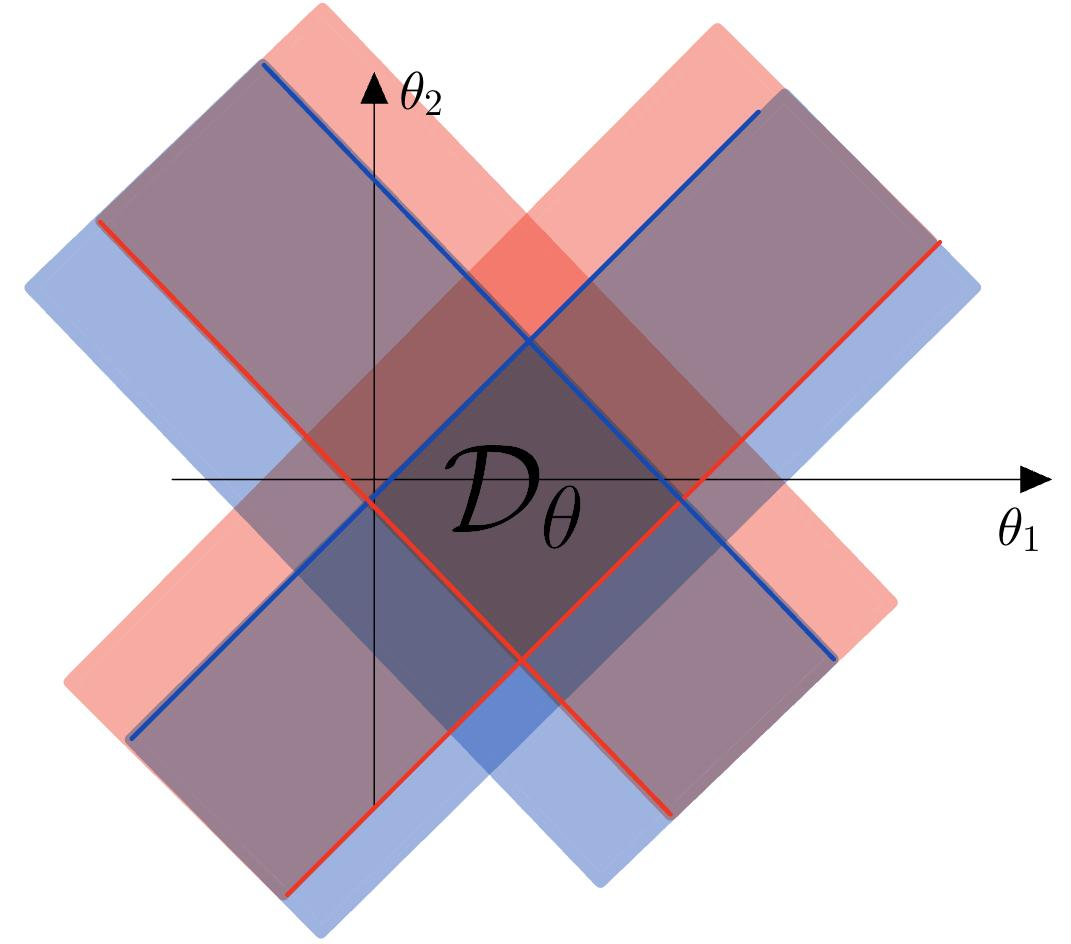
\includegraphics[scale=0.2]{img/polytope1.jpeg}
    \caption{$\mathcal{D}_\theta$ resulting from a pair of equations}
\end{figure}

{\color{blue}
\noindent
Let us remind that the FPS for sure contains $\theta_{true}$
if and only if all the a-priori assumptions are correct, otherwise the FPS will be \textbf{empty}!}\\
It is remarkable, that this was a case in which by inspection you can read the $PUI$, however we need to generalize. In particular the problem of finding a $PUI$ in the hypotesis of LTI systems with equation error noise structure can be recasted in the solution of \textbf{two standard Linear Programming (LP) problems}: minimization of a linear (convex) objective under constraints representing a polytope.\footnote{
    \noindent
    A \textbf{Linear Programming (LP) problem} is a convex optimization problem of the form
    \begin{equation*}
        \min_{x\in\mathbb{R}^n} {c^T{x}} \quad \text{subject to} \ Ax \le b
    \end{equation*}
    This takes into account all the situations when the problem can be \textit{exactly written} as the minimization of a \textbf{linear function} of the optimization variable subject to \textbf{a set of linear inequalities and/or equalities constraints}.
}

\section{PUIs computation by mean of LP problems solution} 
We know that for a certain parameter $\theta_j$, $j=1,...,p$,  the related interval is $PUI=[\underline{\theta}_j, \overline{\theta}_j]$. Under assumption of having a LTI system with Unknown But Bounded error.
\begin{align}
    \label{eq:th_under}
    &\underline{\theta}_j \doteq \min_{\theta\in\mathcal{D}_\theta} \theta_j= \min_{\theta\in\mathbb{R}^n} \theta_j 
    \qquad \qquad \qquad  \text{s.t.} \begin{cases}
        \tilde{y}(k)+... \le \Delta_e\\
        \tilde{y}(k)+... \le -\Delta_e
    \end{cases} \ k=n+1, ..., N\\
    \label{eq:th_over}
    &\overline{\theta}_j \doteq \max_{\mathcal{D}_\theta} {\theta_j} = \max_{\theta\in\mathbb{R}^n} {\theta_j}=\min_{\theta\in\mathbb{R}^n} {-\theta_j} 
    \quad  \text{s.t.} \begin{cases}
        \tilde{y}(k)+... \le \Delta_e\\
        \tilde{y}(k)+... \le -\Delta_e
    \end{cases} \ k=n+1, ..., N
\end{align}

\noindent
Note that both the problems (\ref{eq:th_under}) and (\ref{eq:th_over}) can be rewritten in the form of an LP problem by suitably choosing $c$ and by arranging the set of constraints in suitable matrices $A$ and $b$. For example when we want to compute the PUI for the $\theta_1$ parameter for a first order system, the direction $c$ will be $c=[1 \quad 0]^T$, then for $\theta_2$, $c=[0 \quad 1]^T$. In \texttt{MATLAB} once you have formulated the problem in the LP form, you can use the command \texttt{[th, opt\_val]=linprog(c,A,b)}, in which \texttt{th} is the optimal solution, while \texttt{opt\_val} is the optimization variable.\\
In conclusion, we have understood that the problem of finding the PUIs for $p$ parameters in the described setting, is leading to the solution of $2p$ LP problems, whose solutions are \textbf{global ones}, the problem in this case can be exactly solved without adding any conservativeness!\\

\noindent
The most critical issue of using such an approach is that, despite any type of experimental set-up can be recasted into a model having an equation error noise structure, I rarely am able to retrieve a bound $\Delta_e$. \\
{\color{blue}
More in particular, this approach can be applied all the times you have that the model is linearly parametrized, that is \textit{the parameters appears linearly in the equation}, since from the regression form you have samples from the input and output which can be for sure non linear ones! 
}


\section{Final remarks}
In this section we have introduced the \textit{Set-Membership approach} for the model parameters estimation. Next, we have analysed the main ingredients, and introducing the concept of \textbf{Feasible parameter set} we have understood that such an approach leads with itself a robust way for describing the parameters, embedding the uncertainty which comes from the data collection. This has been carried out by properly defining the \textit{Parameter Uncertainty Interval}. \\

In the last part we have applied all of the features of the described approach starting from the simplest case in which the model to be identified was LTI and the noise samples unknonwn but bounded. By suitably arranging the mathematical constraints derived by putting together all the a-priori and a-posteriori information, we have recasted the problem of finding the PUIs in the solution of a couple of LP problems which leads to a global minima. Finally, analyzing the problem of SM Identification in this way was mainly of theoretical and conceptual interest since we have seen that retrieving a bound $\Delta_e$ on the error is practically impossible. Other approaches embedding a complete description of the noise samples are needed.



\chapter[SM SysId of LTI systems with EIV noise structure]{Set-Membership SysId of LTI systems with Errors-In-Variables (EIV) noise structure}

We have seen in the last chapter that an equation-error noise structure leads to a solution of LP problems for obtaining the Parameter Uncertainty Intervals, however, we have seen that there are some drawbacks. 
First of all the way we can find a bound $\Delta_e$ on the noise samples.
Then, the objective here is to find a way for dealing with the 'original' problem, that is the one using the output and input samples corrupted by noise. In order to gradually present all the needed ingredients for properly solving the problem, we show in turn general teoretical results and examples in which such results are applied to our problem of \textit{System Identification}.

\section{ Feasible Parameter Set in the EIV set-up}
In order to define also for this type of set-up the feasible parameter set, we have to follow the same road as we have done before. In particular we have to put together:
\begin{description}
    \itemsep-0.2em
    \item[A-priori information on the system] We know that the system belongs to a certain class $\mathcal{F}$, moreover we know the order $n$ of the system itself.
    \item[A-priori information on the noise] In particular the way the uncertainty enters the identification problem (we assume here the most general case when both input and output are corrupted by noise) and the boundedness of the noise samples, in particular
    \begin{equation}
        \vert \eta(k) \vert \le \Delta_\eta \quad
        \vert \xi(k) \vert \le \Delta_\xi
        \quad
        \forall k=1,...,N
    \end{equation}
    \item[A-posteriori information] They are nothing but the experimentally collected data $$\tilde{y}(k)=y(k)+\eta(k), \quad 
    \tilde{u}(k)=u(k)+\xi(k) $$
\end{description}
For an \textbf{LTI system of order $n$} the feasible parameter set is defined as follows: 

\begin{equation}\label{eq:FPS}
    \begin{aligned}
        \mathcal{D}_\theta = \{
            &\theta\in\mathbb{R}^p:  
            (\tilde{y}(k)-\eta(k))+\sum_{i=1}^n{\theta_i}\ ({y}(k-i)-\eta(k-i))=\\
            &\sum_{j=0}^m \theta_j \ (u(k-j)-\xi(k-j)), \quad
            k=n+1,...,N
        \} 
    \end{aligned}
\end{equation}
\noindent
In this context the definition of PUI is always the same, and the extrema of such an interval are defined as before by  solving the optimization problems:

\begin{equation*}
    \underline{\theta}_j = \min_{\theta\in\mathcal{D}_\theta} \theta_j, \quad 
    \overline{\theta}_j = \max_{\theta\in\mathcal{D}_\theta} \theta_j
    \Longrightarrow PUI_{\theta_j}=[\underline{\theta}_j,\overline{\theta}_j]
\end{equation*}
At this point the question is: \textbf{what type of $\mathcal{D}_\theta$ I obtain?} 
\section{Extended Feasible Parameter Set $\mathcal{D}_{\theta,\eta,\xi}$}
How we are able to see in the (\ref{eq:FPS}) the set definition depends also on the noise samples. The difference here is that I cannot eliminate them without adding any approximation. Substancially, I am introducing a non trivial number of new unknown in the description of the set: for $N$ collected samples, $2N$ new variables are added, which cannot be eliminated. For this reason we have to \textit{enlarge} the set $\mathcal{D}_\theta$ involving also the new variables. In this way we introduce the so-called \textbf{Extended Feasible Parameter Set (EFPS)} which we indicate with $\mathcal{D}_{\theta,\eta,\xi}$. \\
In order to better understand this aspect, let us consider a toy-example in which we have a single parameter $\eta(1)$ which is added to the pair $\theta_1, \theta_2$. The EFPS in this case -- how the figure below shows -- is a subset of $\mathbb{R}^3$.
\vspace{-0.2cm}
\begin{figure}[h]
    \centering
    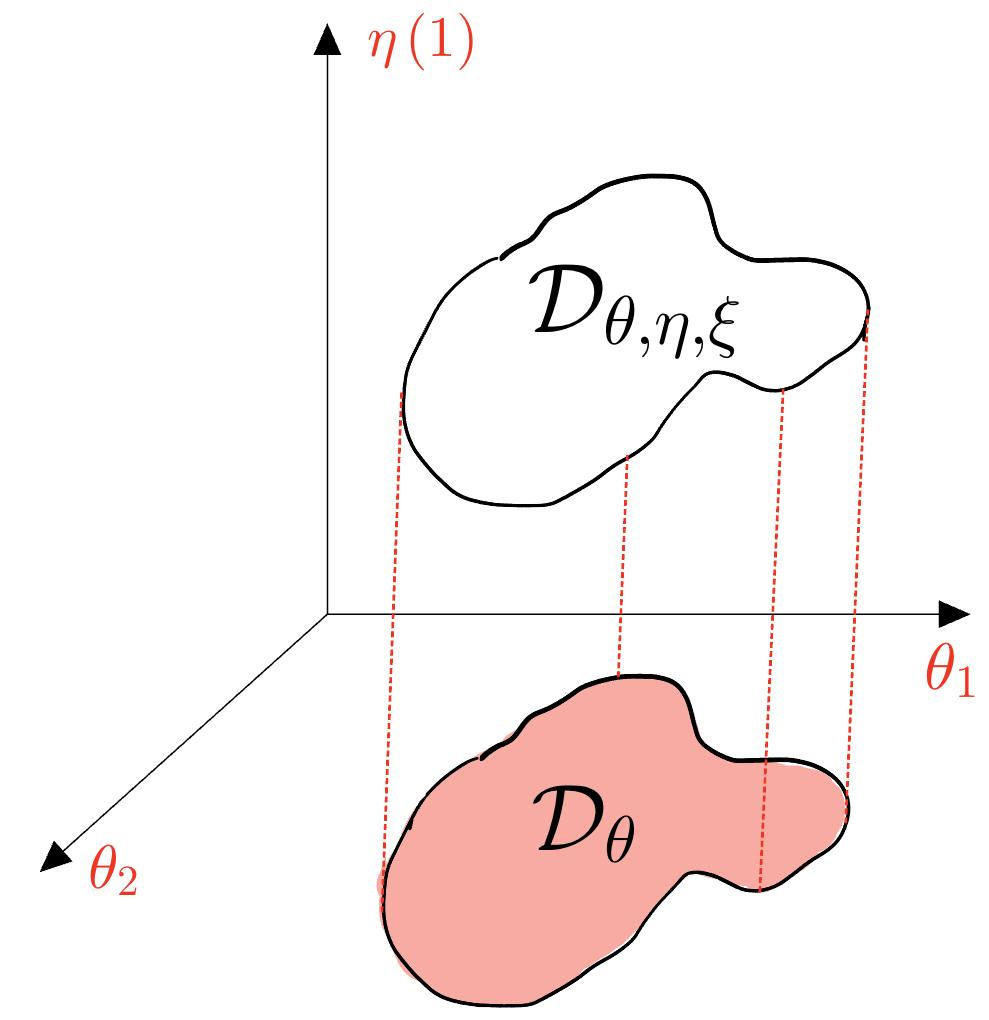
\includegraphics[scale=0.15]{img/EFPS.jpeg}
    \caption{Example in $\mathbb{R}^3$ of the Extended feasible parameter set}
\end{figure}

\noindent
The FPS $\mathcal{D}_\theta$ is nothing but the projection on the $(\theta_1,\theta_2)$ plane of the set $\mathcal{D}_{\theta,\eta}$, in this case no parameter $\xi$ is present.

\noindent
The definition of the \textbf{Extended Feasible Parameter Set} becomes the following:
\begin{equation}
    \begin{aligned}
        \mathcal{D}_{\theta,\eta,\xi} = \{
            &\theta\in\mathbb{R}^p, \eta\in\mathbb{R}^N, \xi \in \mathbb{R}^N: 
            \tilde{y}(k)-\eta(k) + \theta_1 (y(k-1)-\eta(k-1)) +\\
            &+\theta_2 (y(k-2)-\eta(k-2))+\dots+\theta_n (y(k-n)-\eta(k-n))=\\
            &=\theta_{n+1} (u(k)-\xi(k))+\theta_{n+2} (u(k-1)-\xi(k-1)) + ...+\\
            &\theta_{n+m+1} (u(k-m)-\xi(k-m)), \quad k=n+1,...,N\\
             &\vert \xi(k) \vert \le \Delta_\xi, \quad 
            \vert \eta(k) \vert \le \Delta_\eta, \quad k=1,...,N
        \}
    \end{aligned}
\end{equation}

\noindent
Such a set is defined by \textbf{nonlinear} and \textbf{non-convex} constraints and then the set is non-convex. In the specific case, the constraints that arises are \textbf{bilinear ones} which are a particular class of \textbf{polynomial constraints}. In general we know that is very hard to obtain a global minimum from a non-convex optimization problem, in this case using some tools for \textit{polynomial optimization} it is possible to reach a global minimum.\\

\noindent
In this framework the problem of finding the PUIs becomes:
{\large{
    \begin{equation}\label{eq:PUI_delta}
        PUI_{\theta_j} = [\underline{\theta}_j,\overline{\theta}_j] \Longrightarrow 
        \underline{\theta}_j = \min_{{\theta,\eta,\xi}\in\mathcal{D}_{\theta,\eta,\xi} } \theta_j,    \quad
        \overline{\theta}_j = \max_{{\theta,\eta,\xi}\in\mathcal{D}_{\theta,\eta,\xi}} \theta_j
    \end{equation}
}}

\section{Convex relaxation for Polynomial Optimization Problems (POPs)}
\begin{center}
    \textsf{
    In this section we will introduce some general theoretical results on polynomial optimization problems, that -- how we have seen -- are the ones arising in the definition of the extended feasible parameter set (EFPS). We will start by formulating them, we will analyze the type of sets they produce and finally we will introduce the concept of \textbf{convex relaxation}.}
\end{center}

\noindent 
Let us consider the following general optimization problem:
\begin{equation}
    \begin{aligned}
        \min_{x} &f_0(x)\\ 
        &\text{s.t.} \ f_k(x)\le{0} \quad k=1, ..., l\\
        &f_k(x)=0 \quad k=l+1,...,m
    \end{aligned}
\end{equation}
where $f_0$ and $f_k, \ k=1,...,m$ are \textbf{multivariate polynomials} in the optimization variable $x$. Giving an example if $x=[x_1\ x_2\ x_3]^T$, an example of $f_0$ is
\begin{equation*}
    f_0(x)=x_1^2+x_2{x_3^3}+x_1^5{x_2^3}+7{x_3^2}
\end{equation*}
All POPs can be written, for sure, in the so-called \textbf{epigraphic form} by introducing a scalar (slack) variable $\gamma$.

\begin{multicols}{2}
    \noindent
    \textbf{\color{red}Original formulation}
    \begin{equation}
        \begin{aligned}
            \min_{x\in\mathbb{R}^n} &\ f_0(x)\\ 
            &\text{s.t.} \ f_k(x)\le{0} \quad k=1, ..., l\\
            &f_k(x)=0 \quad k=l+1,...,m
        \end{aligned}
    \end{equation}
    \newcolumn\\
    \textbf{\color{red}Epigraphic formulation}
    \begin{equation}
        \begin{aligned}
            \min_{x\in\mathbb{R}^n, \gamma \in \mathbb{R}} &\ \gamma\\ 
            &\text{s.t.} \ f_0(x)\le\gamma\\
            &f_k(x)\le{0} \quad k=1, ..., l\\
            &f_k(x)=0 \quad k=l+1,...,m
        \end{aligned}
    \end{equation}
\end{multicols}
\noindent
By rewriting a generic POP in the epigraphic form, it becomes a problem of \textbf{minimizing a linear function over a non-convex set described by polynomial constraints} (this is also true  for the unconstrained case).

\begin{figure}[h] \label{fig:non-convex}
    \centering
    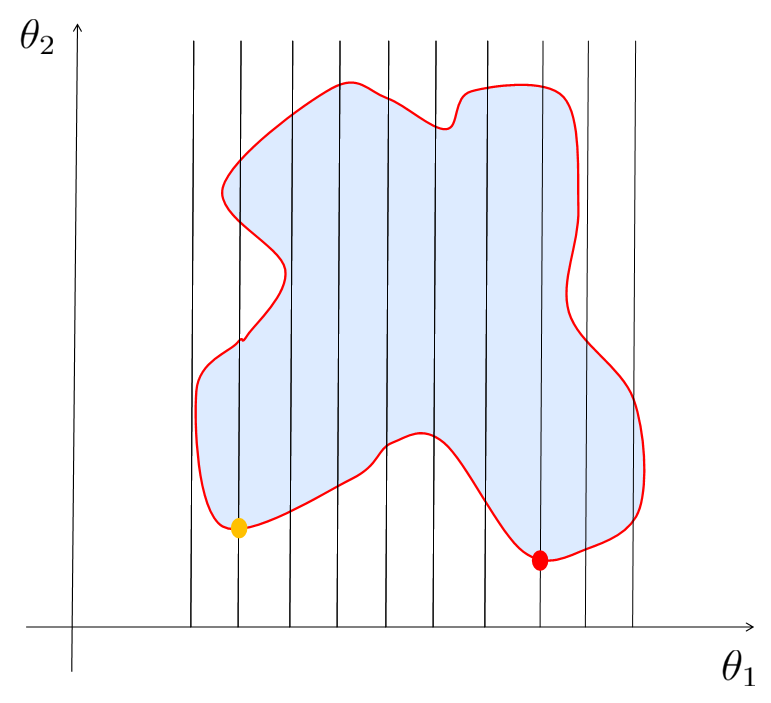
\includegraphics[scale=0.5]{img/nonconvex.png}
    \caption{Example of min a linear objective (thin line) over a non-convex set (sky-blue)}
\end{figure}

The figure (\ref{fig:non-convex}) shows the general idea. We are moving a linear objective (thin lines in black) over the set in sky-blue derived by the polynomial (so non-convex) constraints. The thin lines are the so-called \textit{level-curves} in order to minimize $\theta_1$. Moreover the orange point is a \textbf{local minimum}, while the red one is the \textbf{global minimum}.\\

\noindent
\textbf{\color{red}Important remark:} since a generic POP can written in epigrapigh form, we can note that the non-convexity of  the problem is now \textbf{completely embedded} in the description of the set of constraints $\to$ whether we want to compute the \textbf{global optimal solution} we have to deal with the non-convexity of the set of constraints. It is very high the probability of getting stuck in local minima.\\

\begin{definition}[Convex hull of a non-convex set] Given a non-convex set $\mathcal{S}$, the \textbf{convex hull} for it is the smallest  convex-set including $\mathcal{S}$. 
\end{definition}

A very-nice property is that the \textbf{min/max} computed on the convex hull is equal to the one computed on the original set. In this way we gain the convexity of the problem. 

In other words,if we are able to write down the equations describing the convex hull $C_\mathcal{S}$ of the non-convex set $\mathcal{S}$ we have that:
\begin{equation}
    \min_{x\in{C_\mathcal{S}}} f(x) = \min_{x\in\mathcal{S}} f(x)
\end{equation}
The drawback here is that, in general, obtaining a mathematical description of $C_\mathcal{S}$ is a quite difficult problem.\\
In the particular case of POPs, it is possible to compute a \textbf{convex relaxation os $\mathcal{S}$} depending on a parameter called the \textbf{order of relaxation} $\delta$.

\begin{figure}[h]
    \centering
    \subfigure[Convex hull $C_\mathcal{S}$]{
        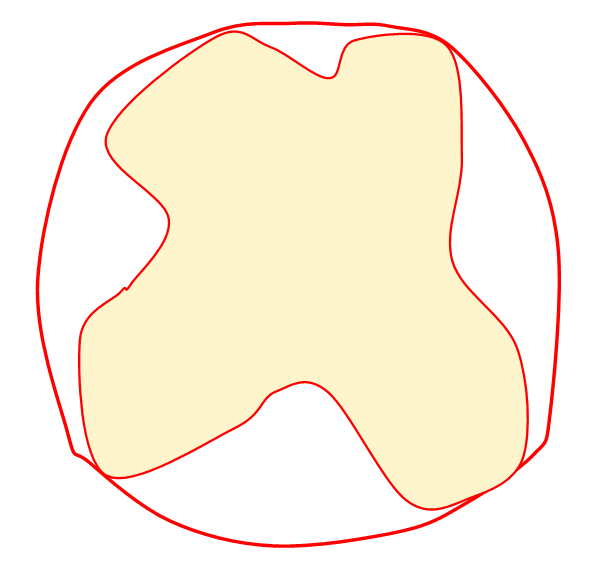
\includegraphics[scale=0.5]{img/convex_hul..png}
    }
    \subfigure[Relaxing the convex hull by $\delta$]{
        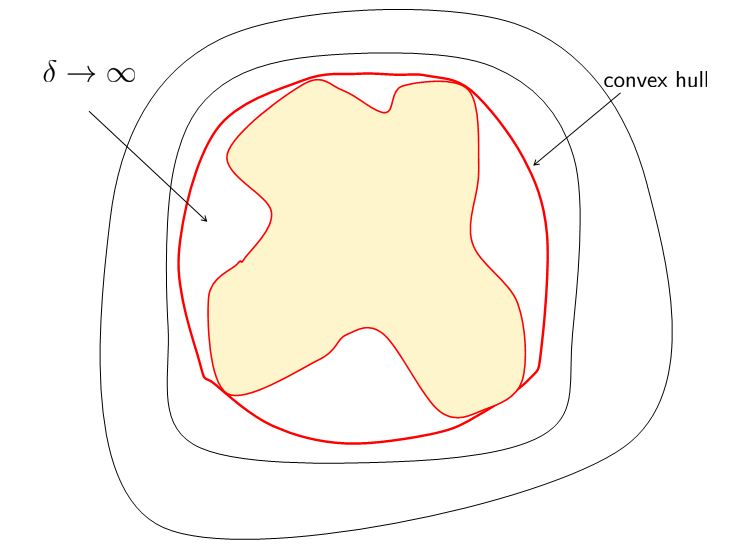
\includegraphics[scale=0.5]{img/relax.png}
    }
\end{figure}
\begin{figure}[h]
    \centering    
\end{figure}

For a given $\delta$ we have different relaxed sets as you can see in the figure, moreover for $\delta\to\infty$ the relaxed set coincides with the convex hull in red.\\
All of this concepts are then applied to our optimization problem which is aimed to find the extrema of the Parameter Uncertainty Intervals for our problem of System Identification. In this case comes up an interesting property, that is, for sure whatever is the order $\delta$, we are including the real PUI. More specifically, we have that for each $k$ the relaxed solutions $\underline{\theta}_k^{\delta}$ and $\overline{\theta}_k^{\delta}$ are such that:
{\large{
    \begin{equation}
        \underline{\theta}_k^{\delta} \le \underline{\theta}_k
        \quad 
        \overline{\theta}_k^{\delta} \ge \overline{\theta}_k
    \end{equation}
}}
moreover it holds that: 
\begin{equation}
    \lim_{\delta\to\infty} \underline{\theta}_k^{\delta} = \underline{\theta}_k \quad
    \lim_{\delta\to\infty} \overline{\theta}_k^{\delta} = \overline{\theta}_k
\end{equation}

\noindent
In order to solve a POP by means of \textit{Lassere convex  relaxation approach} in MATLAB we use:
\begin{enumerate}
    \item \textsf{SparsePOP} that given a polynomial optimization problem and the order of relaxation $\delta$ provides a \textit{Semidefinite relaxed problem (SDP)};
    \item Finally \textsf{SparsePOP} calls the optimization toolbox \textsf{SeDuMi} which solves  the given SDP. 
\end{enumerate}

\section{Choosing the order of relaxation $\delta$}
Let us call $x^*$ the global optimal solution of a given POP, and $x^{\delta}$ the solution of the corresponding convex relaxed solution of order $\delta$. \textbf{How to select $\delta$?} From the theory we know mainly \textbf{three results}:
\begin{description}
    \item[\color{blue}Result 1 \textsf{(R1)}] It holds that:
    \begin{equation}
            \lim_{\delta\to\infty} \  x^\delta \to x^*
    \end{equation}
    this result is not in the most rigorous form since has been proved the convergence for the optimal value, not for the optimal solution. In our case, we are lucky since we are minimizing/maximizing the identity function.
    \item[\color{blue}Result 2 \textsf{(R2)}] The \textit{order of relaxation} $\delta$ must be such that:
    \begin{equation}\label{eq:lower_bound_delta}
        \delta \ge \bigg\lceil \frac{n_{max}}{2}\bigg\rceil =\delta_{min}
    \end{equation} 
    where $n_{max}$ is the maximum degree of the polynomials related to the objective and to the constraints; 
    \item[\color{blue}Result 3 \textsf{(R3)}] the complexity of the SDP problem obtained by applying to the original POP \textit{convex relation techniques} grows exponentially in the order of relaxation $\delta$ and grows exponentially in the number of optimization variables (decision variables) of the original POP. 
\end{description}

\noindent
At this point we can note that such results are, on a certain extent, negative for us since: only making grow $\delta$ we can obtain a good solution, but the complexity of the problem grows exponentially with respect to $\delta$!  
However there is evidence that:\\
\begin{description}
    \item[\color{blue}Result 4 \textsf{(R4)}] For a \textbf{large class of optimization problems} (including the one treated in this course) it is possible to prove that the convergency to the \textbf{global optimal solution} of the original POP is very fast and it is achieved for a finite value of $\delta$. Since we are not able to increase a lot $\delta$, this result helps us a lot. However, keep in mind that there is always the lower bound given by the (\ref{eq:lower_bound_delta}).
\end{description}

\section{Our case: SM SysId with EIV noise structure}
What is the impact in the case we are treating POP arising from SM SysId with EIV noise structure? Since we have seen there are \textbf{bilinear constraints} (order 2 polynomials) arising, we have that $\delta_{min}=1$; furthermore the number of optimization variables, how we have seen in previous paragraph is going to include the parameters, and the samples of the noise, which are in number of $2N$, with $N$ being the number of experimentally collected I/O pairs.\\
Now, since in SysId problems $N$ is going to be quite large in many applications, then the computational complexity is going to be \textbf{untractable}! But we can exploit the following result:
\begin{description}
    \item[\color{blue}Result 5 \textsf{(R5)}] If the original POP satisfies a property called \begin{center}\textbf{running intersection property}\footnote{
        Roughly speaking, even if there a lot of optimization variables, only a small number of them are appearing at the same time in a certain constraint.
    } \end{center}it is possible to build a sequence of convex SDP relaxation involving much less variables. The problem use a lot of matrix with a lot of zeros (\textit{sparse matrices}). This technique is called \textbf{sparse convex relaxation} and it is the one implemented in SparsePOP.
\end{description}

\noindent
SparsePOP software is able to automatically check if the original POP satisfies such a property and if this is the case, it applies the \textbf{sparse convex relaxation}. This allows us to formulate another important result:

\begin{description}
    \item[\color{blue}Result 6 \textsf{(R6)}] The complexity of the SDP problem obtained by applying the \textit{sparse convex relaxation} to the original POP:
    \vspace{-0.3em}
    \begin{itemize}
        \itemsep-0.3em
        \item grows exponentially with the order of relaxation $\delta$ (this, still is a problem); 
        \item grows \textbf{linearly} with the number of optimization variables
    \end{itemize}
\end{description}

The 6th result tells us that the problem \textit{SM-ID for LTI systems with EIV noise structure} is computationally tractable for a rather large number of I/O experimentally collected data since the problem satisfies the \textit{running intersection property} and it is characterized by bilinear constraints.

\section{SM SysId of LTI system with EIV using \texttt{SparsePOP}}
First of all let us write down the FPS and EFPS (respectively what we called $\mathcal{D}_\theta$ and $\mathcal{D}_{\theta, \eta, \xi}$). In order to simplify the notation, but without loss of generality we consider the case where the sytem to be identified is of order $n=2$. The definition of FPS and EFPS are as follows:

\begin{equation} \label{eq:FPS} \tag{\textsf{FPS}}
    \begin{aligned}
        \mathcal{D}_\theta = \big\{&\theta\in\mathbb{R}^5: \ 
            y(k)+\theta_1{y(k-1)}+\theta_2{y(k-2)}
            -\theta_3{u(k)}+\\
            &-\theta_4{u(k-1)}-\theta_5{u(k-2)}=0 \quad k=3,...,N\\
            &\tilde{y}(k) = y(k) + \eta(k), \quad
            \tilde{u}(k) = u(k) + \xi(k), \quad k=1,..., N\\
            &\vert{\eta(k)}\vert \le \Delta_\eta, \quad 
            \vert{\xi(k)}\vert \le \Delta_\xi, \ k=1,...,N
        \big\}
    \end{aligned}
\end{equation}
%-------------------------
\begin{equation}\label{eq:EFPS} \tag{\textsf{EFPS}}
    \begin{aligned}
        \mathcal{D}_{\theta,\eta, \xi} = \big\{
            &\theta\in\mathbb{R}^5,
            \eta \in \mathbb{R}^N, 
            \xi \in \mathbb{R}^N: \
            \tilde{y}(k) - \eta(k) +\theta_1(\tilde{y}(k-1)-\eta(k-1)) \\
            &+\theta_2(\tilde{y}(k-2)-\eta(k-2))-\theta_3(\tilde{u}(k)-\xi(k))+ -\theta_4(\tilde{u}(k-1)-\xi(k-1))\\
            &-\theta_5(\tilde{u}(k-2)-\xi(k-2))=0, \  k=3,...,N \\
            &\vert{\eta(k)}\vert \le \Delta_\eta, \quad 
            \vert{\xi(k)}\vert \le \Delta_\xi, \ k=1,...,N
        \big\}
    \end{aligned}
\end{equation}

\noindent
Now, we have to solve the problems in (\ref{eq:PUI_delta}), for all of the parameters $\theta_j$, $k=1,...,5$. Then, if we have $p$ parameters we have to solve $2p$ optimization problems which are nothing but POPs. Then, we have to properly build data structures \texttt{objPoly} and \texttt{ineqPolySys} containing respectively the information about the \textit{objective function} and the \textit{constraints} of the optimization problem under study.

\subsection{Data structure \texttt{objPoly}}
As far as the PUI are concerned, we know that the objective function is simply, for example:
\begin{equation}
    f_0(\theta)=\theta_1
\end{equation} for the 1$^{st}$ parameter. The \texttt{objPoly} structure must be built as follows:
\begin{verbatim}
objPoly.typeCone=1;                %no use for this field
objPoly.noTerms=1;                  %number of rows of 'supports' matrix
objPoly.dimVar=5+2*N;               %number of colummns of 'supports' matrix
objPoly.degree=1;                   %degree for the objective function
support=zeros(objPoly.dimVar,1);
support(1)=1;                       %for the first parameter
objPoly.supports=support;           %[1 0 0 ... 0]
objPoly.coef=[1;0;0;0;0;...;0]
\end{verbatim}

\subsection{Data structure \texttt{ineqPolySys}}
In the following we are building the part of \texttt{ineqPolySys} related to the first constraint ($k=3$). Here the \texttt{supports} matrix is not so easy to show, since it is very big! We will use dots in order to have a sort of 'contraction' of such a matrix, with the aim to understand what are its features. The fields to fill in are exactly the same with respect to \texttt{objPoly}. The constraint for which the data structure is built is:
\begin{equation}
    \begin{aligned}
        &\tilde{y}(3) - \eta(3) +\theta_1\tilde{y}(2)-\theta_1\eta(2) +\theta_2\tilde{y}(1)-\theta_2\eta(1)-\theta_3\tilde{u}(3)+\theta_3\xi(3)+ \\
            &-\theta_4\tilde{u}(2)+\theta_4\xi(2) -\theta_5\tilde{u}(1)+\theta_5\xi(1)=0
    \end{aligned}
\end{equation}

\begin{verbatim}
ineqPolySys{1}.typeCone=-1;     %equality --> -1  | inequality --> 1
ineqPolySys{1}.noTerms=12; 
ineqPolySys{1}.dimVar=5+2*N;
ineqPolySys{1}.degree=2; 
ineqPolySys{2}.supports=support; 
ineqPolySys{2}.coef=coef;
\end{verbatim}

\noindent
The field \texttt{support} and \texttt{coef} are defined as follows: 
{\small{
    \begin{equation*}
        \texttt{support}=\begin{bmatrix}
            &{\color{blue}\theta_1}&{\color{blue}\theta_2}&{\color{blue}\theta_3}&{\color{blue}\theta_4}&{\color{blue}\theta_5}&{\color{blue}\eta(1)}&{\color{blue}\eta(2)}&{\color{blue}\eta(3)}&{\dots}&{\color{blue}\eta(N)}&{\color{blue}\xi(1)}&{\color{blue}\xi(2)}&{\color{blue}\xi(3)}&{\cdots}&{\color{blue}\xi(N)}\\
            {\color{blue}\tilde{y}(3)}              &0&0&0&0&0&0&0&0&0&0&0&0&0&0&0\\
            {\color{blue}- \eta(3)}                 &0&0&0&0&0&0&0&{\color{red}\textbf{1}}&0&0&0&0&0&0&0\\
            {\color{blue}\theta_1\tilde{y}(2)}      &{\color{red}\textbf{1}}&0&0&0&0&0&0&0&0&0&0&0&0&0&0\\
            {\color{blue}-\theta_1\eta(2)}          &{\color{red}\textbf{1}}&0&0&0&0&0&{\color{red}\textbf{1}}&0&0&0&0&0&0&0&0\\
            {\color{blue}\theta_2\tilde{y}(1)}      &0&{\color{red}\textbf{1}}&0&0&0&0&0&0&0&0&0&0&0&0&0\\
            {\color{blue}-\theta_2\eta(1)}          &0&{\color{red}\textbf{1}}&0&0&0&{\color{red}\textbf{1}}&0&0&0&0&0&0&0&0&0\\
            {\color{blue}-\theta_3\tilde{u}(3)}     &0&0&{\color{red}\textbf{1}}&0&0&0&0&0&0&0&0&0&0&0&0\\
            {\color{blue}\theta_3\xi(3)}            &0&0&{\color{red}\textbf{1}}&0&0&0&0&0&0&0&0&0&{\color{red}\textbf{1}}&0&0\\
            {\color{blue}-\theta_4\tilde{u}(2)}     &0&0&0&{\color{red}\textbf{1}}&0&0&0&0&0&0&0&0&0&0&0\\
            {\color{blue}\theta_4\xi(2)}            &0&0&0&{\color{red}\textbf{1}}&0&0&0&0&0&0&0&{\color{red}\textbf{1}}&0&0&0\\
            {\color{blue}-\theta_5\tilde{u}(1)}     &0&0&0&0&{\color{red}\textbf{1}}&0&0&0&0&0&0&0&0&0&0\\
            {\color{blue}\theta_5\xi(1)}            &0&0&0&0&{\color{red}\textbf{1}}&0&0&0&0&0&{\color{red}\textbf{1}}&0&0&0&0
        \end{bmatrix}
    \end{equation*}
}
}

\noindent
As you can note such a matrix is a \textbf{sparse} one, since it has few non-zero elements. Finally the \texttt{coef} vector is:
{{
    \begin{equation*}
        \texttt{coef}=\begin{bmatrix}
            \tilde{y}(3)&-1& \tilde{y}(2)& -1 &\tilde{y}(1) & -1& -\tilde{u}(3) & 1& -\tilde{u}(2) & 1 & -\tilde{u}(1) & 1
        \end{bmatrix}^\textsf{T}
    \end{equation*}
}}
Such a procedure must be repeated for all of the equality/inequality constraints of the problem. It is clear that a piece of code using a \texttt{for} cycle can help significantly in building such data structures! 

\subsection{Data structures \texttt{lbd},\texttt{ubd}, \texttt{param} }
\noindent
Other data structures to be provided to the \texttt{sparsePOP()} command are \texttt{lbd}, \texttt{ubd}, \texttt{param}. As far as the first pair (lower and upper bounds on the optimization variables), you have to use $\pm{10}^{10}$ in order to indicate $\pm{\infty}$ for the parameters $\theta_i$, for the samples $\eta$ and $\xi$ the bounds $\pm\Delta_\eta$ and $\pm\Delta_\xi$ must be used. As far as \texttt{param} is concerned:
\begin{verbatim}
param.relaxOrder=1;                     %order of relaxation (>=delta_min)
param.POPsolver='active-set';           %type of solver to be used
\end{verbatim}

\subsection{Retrieving the solution of the problem}
Once all of the data structures have been built, we can call the \texttt{sparsePOP} command as follows: 
\begin{verbatim}
    [param,SDPobjValue,POP,cpuTime,SDPsolverInfo,SDPinfo] = ...
            sparsePOP(objPoly,ineqPolySys,lbd,ubd,param);
\end{verbatim}

\noindent
In order to retrieve the (refined) solution of the optimization problem:
\begin{itemize}
    \itemsep0em
    \item \texttt{POP.objValueL} contains the \textbf{optimal solution} of the optimization problem\footnote{\texttt{theta\_min(i)=POP.objValueL} if you use a vector to store the $\underline{\theta}_i$. \textbf{Important: } when you are computing $\overline{\theta}_i$ you must write \texttt{theta\_max(i)=-POP.objValueL}. Due to the structure of the problem also \texttt{POP.xVectL} can be used, it is not necessary the change of sign that instead is needed in the \texttt{coef} vector};
    \item \texttt{POP.xVectL} contains the \textbf{optimizer} (minimizer in our case); 
\end{itemize}


 
\chapter[SM SysId of MIMO LTI systems with EIV noise structure]{Set-Membership Identification of MIMO LTI systems with EIV noise structure}

\begin{quotation}
    \textsf{\noindent Till now we have introduced fundamental aspects about Set-Membership Identification, we have understood why it is the most realistic approach to the SysId, and -- in order to go step by step -- we focused our attention on a specific case on which we developed the theory: \textit{SISO LTI systems with Errors-in-variables noise structure.} Our objective now is trying to generalize such results, including the case in which the system to identify is multi-input multi-output (MIMO) or nonlinear. In this chapter we treat the former topic.
    }
\end{quotation}

\noindent
Let us start introducing some general concepts and definition useful for the comprehension of the incoming topics. A \textbf{Multi-Input Multi-Output (MIMO)} Linear Time-Invariant system with $p$ inputs and $q$ outputs can be described by means of a \textit{matrix transfer function} $G(q^{-1})$ where each element represents a SISO transfer function 
\begin{equation}
    G_{ij}(q^{-1})=\frac{N_{ij}(q^{-1})}{D_{ij}(q^{-1})}
\end{equation} 
between the $j$-th input and the $i$-th output.\\
The I/O relationship of the system we want to study is defined by the following equation:
\begin{equation} \label{eq:MIMO_IO}
    \begin{bmatrix}
        y_1\\y_2\\\vdots\\y_q 
    \end{bmatrix}=\underbrace{\begin{bmatrix}
        G_{11}(q^{-1})&G_{12}(q^{-1})&\dots&G_{1p}{(q^{-1})}\\
        G_{21}(q^{-1})&G_{22}(q^{-1})&\dots&G_{2p}(q^{-1})\\
        \vdots&\vdots&\ddots&\vdots\\
        G_{q1}(q^{-1})&G_{q2}(q^{-1})&\dots&G_{qp}(q^{-1})
    \end{bmatrix}}_{G(q^{-1})}\begin{bmatrix}
        u_1\\u_2\\\vdots\\u_p
    \end{bmatrix}
\end{equation}
A block diagram representation of a MIMO system is reported below: 

\begin{figure}[h]
    \centering
    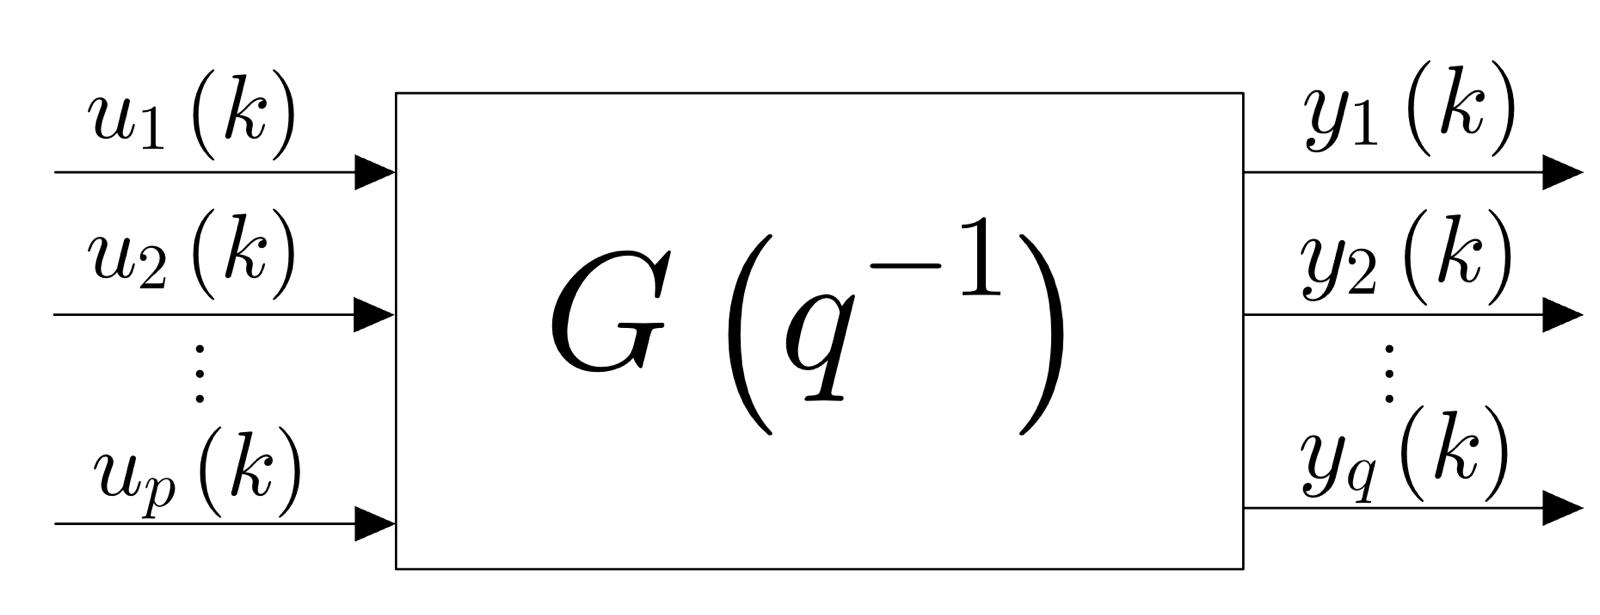
\includegraphics[scale=0.15]{img/MIMO.jpg}
    \caption{Block diagram for a MIMO system}
\end{figure}

\noindent
The reason why I use directly a transfer function description for the system I want to identify is the same for which we use it in the simple case of a SISO LTI system: since we are able to do some open-loop experiments on the plant collecting I/O data, an I/O description such as the \textit{regression form} (that leads to a transfer function) is the most convenient way to mathematically describe the system itself!\\
However, we can have an objection in the sense that we can find an (apparently) \textbf{useful insight} if we start from a state-space description, roughly speaking using the matrices $A,B,C,D$. Indeed, recalling what is the definition of (matrix) transfer function $H(s)$ obtained starting from the state space description we know that:
\begin{equation*}
    \underbrace{H(s)=C(sI-A)^{-1}{B}+D}_{\textsf{continuous time}}, \quad
    \underbrace{H(z)=C(zI-A)^{-1}B+D}_{\textsf{discrete time}} 
\end{equation*}
(From now on without loss of generality, for sake of simplicity we will use $(sI-A)$ for the explanation of what follows).
By computing the inverse of the matrix $sI-A$ we have to divide it by its determinant $\det(sI-A)$ (which is also the \textit{characteristic polynomial}). For this reason all of the elements of $H(s)$ have the same common denominator, resulting into the same parameters to be estimated! \\
Now, at the end of the day our problem is \textit{estimating some parameters} exploiting I/O experimental data. The approaches I can use in order to continue developing the theory are:
\begin{enumerate}
    \itemsep-0.3em
    \item Considering the denominators of the transfer functions \textbf{identical} how the state-space insight suggests us (this plays the role of an additive a-priori information); 
    \item Considering the transfer functions as having \textbf{different denominators} resulting in a greater number of parameters to be estimated.
\end{enumerate}

\noindent
It would be better to analyze the features for one approach and for the other. We can say that the most evident advantage in considering the same all of the denominators is that we have \textbf{less parameters} entering the identification procedure. On the other hand, in the second case we could have \textbf{some physical a-priori information} that suggest us something about the order of each transfer function, the order $n$ in general can be different from one transfer function to another. In such a case we know something directly related to the number of parameters to be estimated\footnote{
    For a system of order $n$, I have $2n+1$ parameter to estimate.
}. Apparently, we are anyway tempted to say that such an information is not lost in the first case, since there could be \textbf{zero-pole cancellations} which makes also very different the several transfer functions. However this is not true, since our collected data are affected by noise and then the parameters related to the zeros/poles are not exact. It is sufficient to think about the fact we retrieve some PUIs from the Set-Membership procedure, uncertainty is embedded into the problem. This evidence suggests us that maybe the best path to be followed is not the one that apparently makes the identification problem simpler. \textit{We will going on discussing the problem following the second approach.}\\

\noindent
Starting from the (\ref{eq:MIMO_IO}), a generic output of the system $y_i$ is given by:
\begin{equation}
    y_i(k)=G_{i1}(q^{-1})u_1(k)+G_{i2}(q^{-1})u_2(k)+\dots+G_{ip}(q^{-1})u_p(k), \quad i=1,...,q
\end{equation}
From this follows an \textbf{important remark}: each output $y_i$ depends on the past samples of the output itself and the samples of the inputs $u_1,...,u_p$ not by the other outputs. In other words the $y_i$ behaviours are \textbf{independent}. Therefore, a first conclusion can be drawn: \textit{the identifiction of a MIMO LTI system with $q$ outputs is equivalent to the identification of $q$ \textbf{MISO} (Multi-input single-output) systems}. Now, the sub-problem to be faced is:

\section{SM Identification of MISO LTI systems}
As usual in a set-membership identification procedure we have to list all of the ingredients of our problem and then put them together to obtain the feasible parameter set. This is the what we are going to do.

\subsection{A-priori information on the system}
The system order $n$ is assumed to be known moreover the I/O mapping can be expressed as follows: 
\begin{equation}
    y=G(q^{-1})\begin{bmatrix}
        u_1\\\vdots\\u_p
    \end{bmatrix} = \begin{bmatrix}
        G_1(q^{-1})&G_2(q^{-1})& \dots & G_p(q^{-1})
    \end{bmatrix}\begin{bmatrix}
        u_1\\\vdots\\u_p
    \end{bmatrix}
\end{equation}
where the function $G_i(q^{-1})$ is:
\begin{equation}\label{eq:Gi}
    G_i(q^{-1}) = \frac{
        \beta_0^i+\beta_1^i{q^{-1}}+...+\beta_{n_i}^i{q^{-n_i}}
    }{1+\alpha_1^i{q^{-1}}+...+\alpha_{n_i}^i{q^{-n_i}}
    }, \quad i=1,...,p
\end{equation}
$n_i\le{n}$ is the dynamical order of $G_i(q^{-1})$. The fact that $n_i$ could be smaller is derived from some other a-priori information, otherwise we put always $n_i=n$ for that function we do not know other insights.

\subsection{A-priori information on the noise}
With the objective of being as more general as possible, we analyze the case \textbf{errors-in-variables} (EIV) where both the inputs and the output are affected by measurement noise. A block diagram showing this set-up is given here:
\begin{figure}[h]
    \centering
    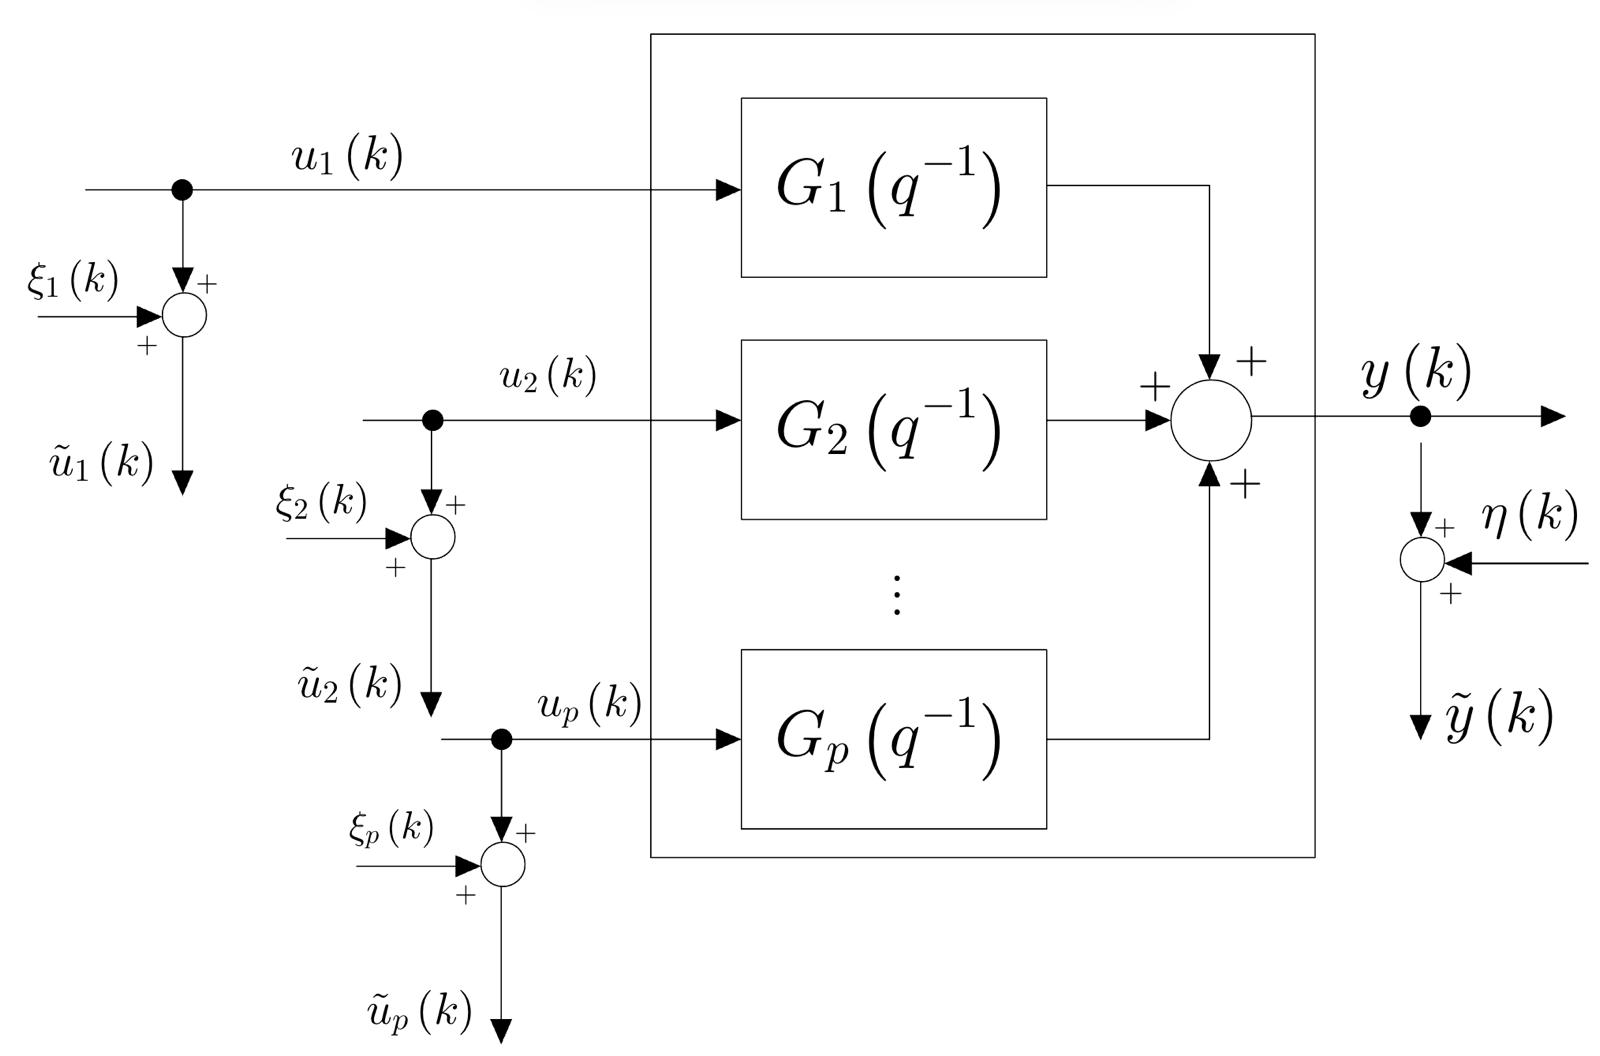
\includegraphics[scale=0.19]{img/MISO.jpg}
    \caption{Block diagram of a MISO LTI system with EIV noise structure}
\end{figure}

%TODO: figura MISO system with EIV noise structure
As in the SISO case we make some quite realistic assumptions on the boundedness of the noise samples, that is:
\begin{equation}
    \begin{aligned}
        &\vert \eta(k) \vert \le \Delta_\eta, \quad k=1,...,N\\
        &\vert \xi_i(k) \vert \le \Delta_{\xi_i} \quad k=1,...,N \quad i=1,...,p
    \end{aligned}
\end{equation}
where $N$ as usual is the number of I/O collected data, and $\Delta_{\eta}, \ \Delta_{\xi_i}$ are the only available information on the noise.

\subsection{A-posteriori information: experimental data}
In order to perform the identification $N$ samples of the inputs $\tilde{u}_1(k), ..., \tilde{u}_p(k), \quad k=1,...,N$ and the output $\tilde{y}(k)$ must be collected by doing an \textit{open-loop experiment} on the plant to be identified.

\subsection{Feasible Parameter set $\mathcal{D}_\theta$}
The next step is to put everything together in order to define the \textbf{feasible parameter set} $\mathcal{D}_\theta$:
\begin{equation}
    \begin{aligned}
        \mathcal{D}_\theta = \big\{
            \theta\in\mathbb{R}^{\sum_{i=1}^p{2n_i+1}}: \quad  
            &y(k)=G_1(q^{-1})u_1(k)+...+G_p(q^{-1})u_p(k),  \quad k=2n+1,...,N\\
            &y(k)=\tilde{y}(k)-\eta(k), \quad
            u_i(k)=\tilde{u}_i(k)-\xi_i(k), \quad i=1,...,p\\
            &
            \vert \eta(k) \vert \le \Delta_\eta, \quad \vert \xi_i(k) \vert \le \Delta_{\xi_i} \quad k=1,...,N \quad i=1,...,p
        \big\}
    \end{aligned}
\end{equation}
More explicitly we can substitute the transfer functions $G_i(q^{-1})$ with the definition we gave in (\ref{eq:Gi}), the set becomes:
\begin{equation}
    \begin{aligned}\label{eq:FPS_MIMO2}
        \mathcal{D}_\theta = \big\{
            &\theta\in\mathbb{R}^{\sum_{i=1}^p{2n_i+1}}: \quad
            y(k)={
                \frac{
                    \beta_0^1+\beta_1^1{q^{-1}}+...+\beta_{n_1}^1{q^{-n_1}}
                }{1+\alpha_1^1{q^{-1}}+...+\alpha_{n_1}^1{q^{-n_1}}
                }
            }u_1(k)+\\
            &+\dots
            +{
                \frac{
                    \beta_0^p+\beta_1^p{q^{-1}}+...+\beta_{n_p}^p{q^{-n_p}}
                }{1+\alpha_1^p{q^{-1}}+...+\alpha_{n_p}^p{q^{-n_p}}
                }
            }u_p(k),  \quad k=2n+1,...,N\\
            &y(k)=\tilde{y}(k)-\eta(k), \quad
            u_i(k)=\tilde{u}_i(k)-\xi_i(k), \quad i=1,...,p\\
            &
            \vert \eta(k) \vert \le \Delta_\eta, \quad \vert \xi_i(k) \vert \le \Delta_{\xi_i} \quad k=1,...,N \quad i=1,...,p
        \big\}
    \end{aligned}
\end{equation} 
Starting from this point, how can we going on? Also in this case we could be tempted in modeling the MISO as a set of SISO, but there are some drawbacks: 
\begin{itemize}
    \item Keep in mind that for a system of order $n$ we have to solve $2(2n+1)$ optimization problems for finding the parameter uncertainty intervals, then this will result in a high computation load; 
    \item The temptation raises up from the moment that we grasp to the \textit{superposition principle for LTI systems} according which if we apply the inputs one at a time, the output will show a behaviour which is related only to that input itself. Unfortunately, in real-world applications is not always possible to "turn-off" some inputs while keeping unchanged the system, this is also because the great majority of the plants are \textit{only approximatively linear}.
\end{itemize}

Another attempt could be doing the common denominator in  (\ref{eq:FPS_MIMO2}) and solving a unique huge identification problem. Again, still there are problems! The dimension of the problem quckly would explode making unsuitable \texttt{SparsePOP} for solving the problem exploiting convex relaxation techniques. Something different is needed... 

\chapter[SM-ID of block structured nonlinear systems]{Set-membership identification of block structured nonlinear systems}

\section{Introduction}
Let us continue to generalize our Set-Membership identification framework introducing the theoretical concepts useful to identify \textbf{SISO nonlinear systems} in the regression form we have seen in the very first part of these notes:

\begin{figure}[h]
   \centering
   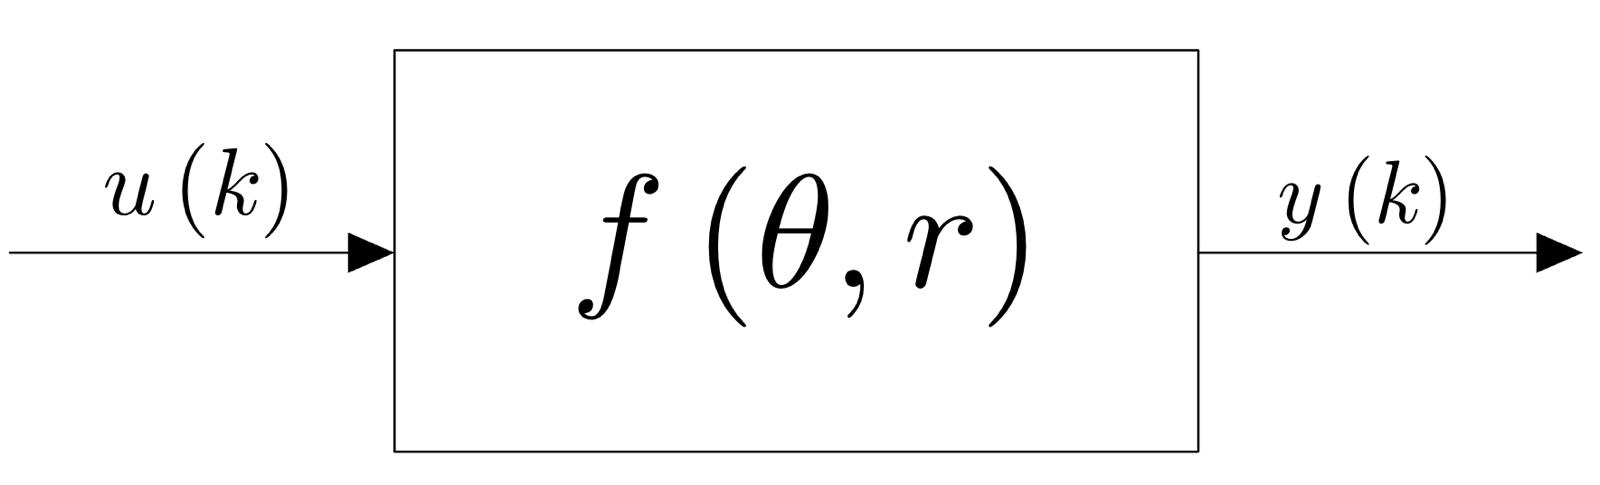
\includegraphics[scale=0.15]{img/nonlinear.jpeg} 
   \caption{Nonlinear SISO system (regression form)}
\end{figure}
\vspace{-1cm}
\begin{equation}
    y(k)=f(\theta,r(k))=f(\theta, [y(k-1),y(k-2),\dots,y(k-n), u(k), u(k-1), \dots, u(k-m)])
\end{equation}
where $\theta$ is the vector with the parameters of the model, while $r(k)$ is the so-called \textbf{regressor}. We specialize the class $f$ of functions we deal with, in particular they are \textbf{multivariate polynomial function of the regressor $r(k)$}. In this context we propose some examples which, as usual, are useful to both introduce and better clarify the setting to which we are approaching. Through all of the examples we do two fundamental quantities are:
\begin{itemize}
    \item The \textbf{dynamical order of the system} $n$; this is related to the number of past samples we need in order to describe the generic system output $y(k)$; 
    \item The \textbf{degree} (or \textbf{order}) $\deg(f)$ of the multivariate polynomial $f$ describing the nonlinear system in the parametrized form.
\end{itemize}

\subsubsection{Example 1}
Suppose that from the physical insights we know that the system has $n=1$ and $\deg(f)=2$. This is the same to state that the equation describing the I/O of the system is:
\begin{align}
    y(k)&=f(\theta,r(k))=f(\theta,[y(k-1),u(k),u(k-1)])=\\
    &=\theta_1y(k-1)+\theta_2 u(k) + \theta_3 u(k-1) 
    + \theta_4 y^2(k-1)+\theta_5 u^2(k)+\theta_6 u^2(k-1)+\\
    &+\theta_7{y(k-1)u(k)}+\theta_8{y(k-1)u(k-1)}+\theta_9{u(k)u(k-1)}
\end{align}

Since $\deg(f)=2$, in order to avoid loosing of generality we have to consider also the mixed monomial terms of order 2.

\subsubsection{Example 2}
Let us consider, now, the case in which both the dynamical order and multivariate polynomial degree are the same as before, on the other hand from the physical insights we know that the structure of the I/O equation is:
\begin{equation*}
    y(k)=\theta_1y(k-1) + \theta_2 u(k) +\theta_3 u^2(k-1)+\theta_4{y(k-1)u(k)}
\end{equation*}
It is not said that all of the terms are present, in this case there is some reason for which this happens.

\subsubsection{Example 3}
Finally, here we consider the case in which, again, $n$, $\deg(f)$ are equal while not having any useful physical insights which can allow us make a guess on the shape of $f(\theta,r)$.
In this particular case some general assumptions on the continuity\footnote{
    for example $f\in\mathcal{C}^0$ or $f\in\mathcal{C}^1$
} of $f$ are needed, otherwise we cannot say anything and the identification problem is not tractable. This example gives the possibility to introduce to cite an important result.

\section{Dealing with nonlinearity of the problem}
Whether one can assume that the function $f$ can leverage on some continuity properties,the \textbf{Stone-Weirstrass theorem} can be used. It allows us with the possibility to approximate as well as we want the true nonlinear function with a multivariate polynomial over a \textit{compact set}. In spite this is a nice result, it is not going to provide a way to build such polynomial, since it is an \textit{existency theorem}.

\subsection{On the choice of the polynomial structure}
When we are not provided with physical insights making us to neglect some terms of the multivariate polynomial, we can always start from a \textit{complete description}, next when the identification procedure is performed, the terms which are not included into the model description will have an uncertainty interval whose central estimate is approximatively equal to zero.

Having said that, the choice of $\deg(f)$ can be done by using the following \textbf{procedure}: 
\begin{enumerate}
    \item[0.] We can start from $\deg(f)=2$\footnote{
        If there was $\deg(f)=1$ the system under study is linear
    } and we try to solve the problem going through the computation of the feasible parameter set $\mathcal{D}_\theta$ putting together all the available information;\item[1.]\textbf{\large Is the $\mathcal{D}_\theta$ empty?}\footnote{
        Practically speaking, using \texttt{SparsePOP} a symptom of the fact that $\mathcal{D}_\theta=\varnothing \ \iff $ POP infeasible can be read in the output variable \texttt{exitflag}, in particuar its negativeness implies the infeasibility of the POP. 
    }
    \begin{itemize}
        \itemsep-0.3em
        \item {\Large{\color{green}\underline{\textbf{NO}}}} In this case we have to check what are the (relaxed) PUI, in particular we have to check that
        \begin{equation} \label{eq:extrema_sign}
            \text{sign}(\underline{\theta}_i) = 
            \text{sign}(\overline{\theta}_i) \quad i=1,\dots,n_\theta
        \end{equation} 
        Whether this is the case we can accept our solution and use the retrieved interval in order to simulate control the identified system. On the other hand, we continue to investigate in the fact that, maybe the the length of the PUI
        \begin{equation}
            \vert \underline{\theta}_i-\overline{\theta}_i \vert \le \delta
        \end{equation}
         for some small $\delta$. In pratice this is the case when, if for the other parameters the property (\ref{eq:extrema_sign}) is fulfilled, the procedure is saying us that $\theta_i=0$. On the contrary if (\ref{eq:extrema_sign}) is not satisfied and the noise bound is big\footnote{
            We can quantify it in percentage terms with respect to the measured input $\tilde{u}(k)$ or output $\tilde{y}(k)$.
         }, it would be better if the sensor is changed because it is not properly measuring the data to be used in the identification process. Finally on the other side when the \textit{sign concordance property} is not fulfilled and the noise relative bound is acceptable, \textbf{the order of the polynomial ought to be increased} $\to$ try $\deg(f)=\deg(f)+1$. 
     \end{itemize} 
    \item {\Large{\color{red}\underline{\textbf{YES}}}} Also in this case the $\deg(f)$ is too \textbf{low}, then you have to increase it.
\end{enumerate}

\noindent
\begin{remark}[\textbf{Unknown dynamical order} $n$]
    A similar \textit{trial and error} approach can also be applied to the case (both linear and nonlinear systems) when the \textit{dynamical order $n$} is not exactly known from the physical insights. This will be useful especially when the Direct Data-driven control technique will be explained.
\end{remark}

\noindent
\subsection{Additional comments on the PUIs extrema sign concordance}
After this discussion, let us give further attention on the property (\ref{eq:extrema_sign}). The reason why we must reject the PUIs with non-concordant sign is that we cannot even know the sign for a certain parameter. Whether we want to design a simple stabilizing \textit{feedback controller}, the fact that we do not have the information on the sign does not protect us from building a positive feedback(!), making unstable the closed loop system. We conclude this part saying that the \textbf{relative size of the uncertainty} is given by: 
\begin{equation}
    \Delta_i = \bigg\vert \frac{\overline{\theta}_i-\underline{\theta}_i}{\theta_i^c} \bigg\vert, \qquad
    \theta_i^c = \frac{\overline{\theta}_i+\underline{\theta}_i}{2}
\end{equation}
where $\theta_i^c$ is the so-called \textbf{central estimate}  which can leverage on some nice properties how we will see in one of the next chapters. When the sign of the extrema is not the same, the uncertainty relative size is greater than the 1 (that is 100\%).


\chapter{Set-Membership identification of continuous time systems}
\chapter{Enforcing stability for the identified model}\label{chap:enforcing}

\textsf{Everytime we perform an open-loop experiment we need BIBO stability otherwise the output of the system to be identified may diverge, so that we are not able to measure it. This is a \textbf{strong information} on the parameters of the system itself! Indeed, adding such an information in the problem allow us to get more \textit{accurate estimate}, that is \textbf{smaller parameter uncertainty intervals} in out Set-Membership framework. The main reference for this part is \citeauthor{cerone2011enforcing} \textit{\citetitle{cerone2011enforcing}, \citedate{cerone2011enforcing} \cite{cerone2011enforcing}}}

\section{Review on stability of Discrete Time LTI systems}
We know that a generic discrete time LTI model can be described by means of a \textit{transfer function} in the z-domain:
\begin{equation}
    G_p(z)=\frac{N(z)}{D(z)}
\end{equation}
\begin{definition}[\textbf{BIBO Stability}]
    $G_p(s)$ is said to be BIBO stable if and only if the response of the system is bounded for all the possible bounded input signals.
\end{definition}

\noindent
Referred to such a definition there is an important result that states: 
\begin{quotation}
    $G_p(z)$ is BIBO stable if and only if the poles of $G_p(s)$ (the roots of $D(z)=0$) have all magnitude less than 1.
 \end{quotation}
\noindent
 It is remarkable that both $N(z)$ and $D(z)$ depends on some parameter $\theta$ to be estimated. In fact:
 \begin{equation}
    G_p(z,\theta)=\frac{N(z,\theta)}{D(z,\theta)}
 \end{equation}
 Thus, we can define a set on the parameter space which is the set of all the parameter values such that the model $G_p(z,\theta)$ is BIBO stable. Such a set can be expressed as
 \begin{equation}
    \mathcal{D}_{\text{stab}}=\{
        \theta\in\mathbb{R}^{n_\theta} : \ D(z,\theta)\ne{0}, \forall{z}\in\mathbb{C}, \ \vert z \vert \ge 1
    \}
 \end{equation}
Henceforth, we can understand that \textbf{stability depends only on the parameters appearing at the denominator} which in turn are the \textit{poles of the system}. Given the denominator of a transfer function $G_p(z)$ there a  theorem (Jury Theorem) by which we can retrieve \textbf{conditions} on the parameters from which it depends, so that the resulting system (for us the system which has been identified) is BIBO stable. 


\section{Jury Theorem}
The \textbf{Jury Theorem} is based on some conditions which rely on a table that is called the \textbf{Jury array}. Before exposing the theorem we give the construction of such an array. 

\subsection{Construction of the Jury array}
The denominator of our transfer function is given by: 
\begin{equation}
    D(z,\theta)=1+a_1{z^{-1}}+a_2{z^{-2}}+\dots+a_n{z^{-n}}
\end{equation}
The following table is the so called \textbf{Jury array}:
\begin{equation}
    {\displaystyle {\begin{array}{lcccccc}
        {\underline {\text{row}}} &\ {\underline {z^{n}}}\ &\ {\underline {z^{n-1}}}\ &\ {\underline {z^{n-2}}}\ &\ \cdots \ &\ {\underline {z^{1}}}\ &\ {\underline {z^{0}}} \\[8pt]
        1 & a_{n} & a_{n-1} & a_{n-2} & \cdots & a_{1} & 1 \\[4pt]
        2 & 1 & a_{1} & a_{2} & \cdots & a_{n-1} & a_{n} \\[10pt]
        3 & c_{n-1} & c_{n-2} & \cdots & c_{1} & c_{0} \\[4pt]
        4 & c_{0} & c_{1} & \cdots & c_{n-2} & c_{n-1} \\[10pt]
        5 & d_{n-2} & d_{n-3} & \cdots & d_{0} & \\[4pt]
        6 & d_{0} & d_{1} & \cdots & d_{n-2} & \\[10pt]
        \!\vdots & \vdots & \vdots & \vdots & \vdots && \\[10pt]
        2n-5 & p_{3} & p_{2} & p_{1} & p_{0} && \\[4pt]
        2n-4 & p_{0} & p_{1} & p_{2} & p_{3} && \\[10pt]
        2n-3 & q_{2} & q_{1} & q_{0} &&&
        \end{array}}}
\end{equation}
We assume that the polynomial at denominator is \textit{monic} so the leading coefficient $a_0$ is always equal to one. Moreover the terms $c$ and $d$ are defined as: 
\begin{equation}
    \begin{aligned}
        &c_{n-1}=\bigg| \begin{matrix}
            a_{n}&a_{n-1}\\
            1&a_{1}
        \end{matrix}\bigg|,  \quad 
        c_{n-1}=\bigg| \begin{matrix}
            a_{n}&a_{n-2}\\
            1&a_{2}
        \end{matrix}\bigg|, \quad 
        c_{n-j}=\bigg| \begin{matrix}
            a_{n}&a_{n-j}\\
            1&a_{j}
        \end{matrix}\bigg|, \quad, \dots, \quad
        c_{0}=\bigg| \begin{matrix}
            a_{n}&a_{1}\\
            1&a_{n}
        \end{matrix}\bigg|\\
        &d_{n-2}=\bigg|\begin{matrix}
            c_{n-1}&c_{n-2}\\
            c_0&c_2
        \end{matrix} \bigg|, \quad 
        d_{n-j}=\bigg|\begin{matrix}
            c_{n-1}&c_{n-j}\\
            c_0&c_j
        \end{matrix} \bigg|, \quad, \dots, \quad
        d_0=\bigg| \begin{matrix}
            c_{n-1}&c_0\\
            c_{0}&c_{n-1} 
        \end{matrix}\bigg| 
    \end{aligned}
\end{equation}
\begin{theorem}[Jury Theorem]\label{th:Jury_thm}
The roots of the polynomial $D(z)$ belong to the \textbf{open unit circle} if and only if the following equations hold:
\begin{enumerate}
    \itemsep-0.2em
    \item $D(z=1)=1+a_1+a_2+\dots+a_n>0$
    \item $(-1)^n D(z=1)=(-1)^n (1-a_1+a_2-a_3+\dots\pm{a_n})>0$
    \item $\vert a_n \vert \le 1$
    \item $\vert c_{n-1} \vert < \vert c_0 \vert$, \ $\vert d_{n-2}\vert < \vert d_0 \vert$, $\dots$, $\vert q_2 \vert < \vert q_0 \vert$
\end{enumerate}
\end{theorem}

\noindent
It is more convenient that the last constraints are recasted in $c_{n-1}^2 < c_{0}^2, \dots$, otherwise it is not so easy to handle such constraints. They keep their non-convex shape, but at least they are polynomial. Finally, it is remarkable that all of the elements of the Jury array are \textbf{polynomial functions of $\theta$}.

\section{SM-ID and Jury theorem derived constraints}
Once we have obtained a strong result on the stability of discrete time systems which are dependent on a certain number of parameters, we can \textbf{enforce stability} of the identified model by: 
\begin{enumerate}
    \itemsep-0.2em
    \item Adding optimization variables representing the entries of the Jury array $c_{n-1}, ..., d_{n-2}, ..., d_0$; 
    \item Modify the extended feasible parameter set in order to include the relation between $\theta$ and the entries of the Jury array $(a_1,...,a_n \to c_{n-1}, ..., c_0)$; 
    \item Adding the relations between different entries of the Jury Array $(c_{n-1},...,{c_0} \to d_{n-2}, ..., d_0 ...)$
    \item Adding the equations (1)-(4) coming from the \textit{Jury Theorem}.
\end{enumerate}

\begin{remark}
    Even if we include these constraints there is no guarantee that the identified model is stable because:
    \begin{enumerate}
        \itemsep-0.2em
        \item We relax our POPs to convex SDP, and so since we are computing an outer approximation of the feasible parameter set, we may fall outside the true FPS, and finding a point (in the parameter space) not satisfying all of the constraints.
        \item Even if we could describe the exact FPS when taking the central estimate, we may fall out of the set.
    \end{enumerate}
\end{remark}

\noindent
Then, \textbf{Why enforcing stability constraints?} They shrink the FPS and ultimately improve the accuracy of the model because the obtained PUI will be tighter.

\section{An applied example}
Given the discrete time LTI system described by
\begin{equation}
    H(z)=\frac{\beta_1{z^{-1}}+\beta_0}{1+a_1{z^{-1}}+a_2{z^{-2}}+a_3{z^{-3}}}
\end{equation}
using the Jury theorem give necessary and sufficient conditions for which the given system is BIBO stable. 
\noindent
The Jury array for the denominator of the given transfer function is:
\begin{equation}
    \begin{matrix}
        a_3&a_2&a_1&1\\
        1&a_1&a_2&a_3\\
        c_2&c_1&c_0
    \end{matrix}
\end{equation}
The necessary and sufficient conditions dictated by the \cref{th:Jury_thm} are:
\begin{equation}
    \begin{cases}
        1+a_1+a_2+a_3>0\\
        -(1-a_1+a_2-a_3)>0\\
        \vert a_3 \vert < 1 \iff -1 < a_3 < 1\\
        \vert c_2 \vert < \vert c_0 \vert \iff c_2^2 < c_0^2
    \end{cases}
\end{equation}
These equations, together with the other describing how the several additive variables and parameters of the system are related, must be embedded into the extended feasible parameter set. Each one of this additive constraints will have its own field of the structure \texttt{ineqPolySys} of \texttt{SparsePOP}.

\part{Direct Data-Driven Control}
\chapter[Direct Data-Driven Control (SM approach)]{Direct Data-Driven Control design: Set-Membership approach}\label{chap:DDDC}

\vspace{-1cm}
\begin{figure}[h]
    \centering
    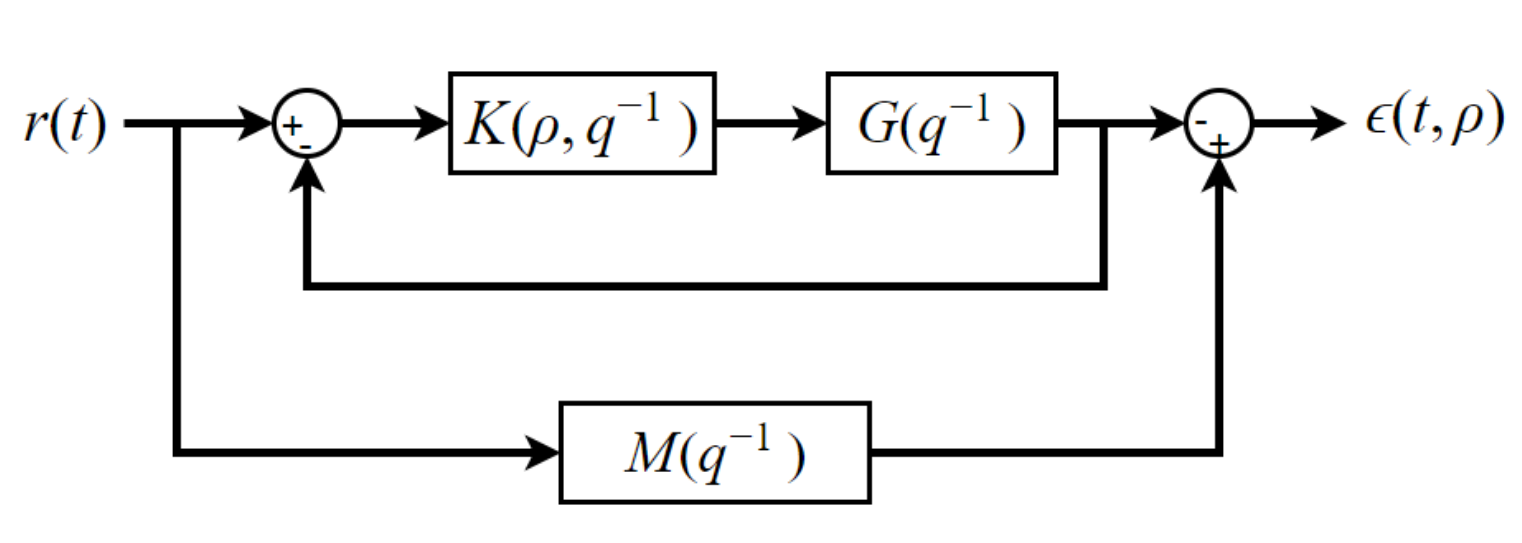
\includegraphics[scale=0.4]{img/DDDC_1.png}
    \caption{Direct Data-Driven Control (DDDC) setting}
    \label{fig:DDDC_setting}
\end{figure}

\begin{quotation}
    \noindent
    \textsf{In the previous chapter we have seen how can we build a model for a dynamical system, linear/nonlinear, SISO/MIMO. For sure, you know that one of the objective of having a mathematical model/description for a given plant is to build a certain \textit{controller} in order to modify the behaviour of the plant itself. In this chapter, going through the description of the \textit{Direct Data-Driven control problem} (DDDC), we will see how to control a certain plant without identify it, but passing directly to the controller design using data.
    }
\end{quotation}

\section{Introduction}
In the field of Control Theory there are mainly three approaches to design a controller for a given plant: 
\begin{enumerate}
    \itemsep-0.2em
    \item \textit{Model-Based technique} in which we have a model for the plant to control, and the problem is solved using some control technique according to the specific problem we have to solve (requirements based, optimal control...);
    \item \textit{Undirect Data-Driven} here since we do not have a model for the plant, at first we retrieve a model  for the plant to be controlled (using some SysId technique), then using the obtained model, some control technique is applied; 
    \item \textit{Direct Data-Driven} Here we have that the controller is designed skipping the plant identification stage, so data are used to build a model directly for the controller.
\end{enumerate}

In particular here the objective, with reference to the \Cref{fig:DDDC_setting} is to design the controller $K$ such that the \textbf{controlled system} could match as well as possible the behaviour of the \textbf{reference model} $M$. In particular given $K(\rho, q^{-1})$, $\rho$ is the \textit{parameter vector} defined as
\begin{equation}
    \rho=[\rho_1 \quad \rho_2 \quad \dots \quad \rho_{n_\rho}]
\end{equation}
\noindent
and we want that 
\begin{equation}\label{eq:approxim}
    T_{ry}(q^{-1})=\frac{G(q^{-1} K(q^{-1}))}{1+G(q^{-1} K(q^{-1}))} \approx 
M(q^{-1})
\end{equation}
Both $K$ and $G$ are assumed to be LTI dynamical systems and the description of $G$ is not available, that is there is no model for the plant to  be controlled. From now on we will assume $M=M(q^{-1})$, $G=G(q^{-1})$ and $K=K(q^{-1})$

\section{Ideal controller $K^*$}
Ideally we want that the \Cref{eq:approxim} could hold with the equality so that
\begin{equation}\label{eq:MMP}
    M=\frac{KG}{1+KG}
\end{equation}
which is the so called \textbf{model matching problem}. We have said that $G$ is not known, but assume for a moment that we are able to know exactly $G$. In this case the model matching problem has a \textit{trivial solution} which corresponds to obtaining an \textbf{ideal controller} $K^*$. By doing simple algebraic manipulation we obtain

\begin{equation}
    M=\frac{GK}{1+GK} \iff M+MGK=GK \iff KG(1-M)=M \iff K^*=\frac{M}{G(1-M)}
\end{equation}
Such a $K^*$ has interesting theoretical property useful in order to go on the description of the DDDC problem, however it can be easily shown that: 
\begin{enumerate}
    \itemsep-0.2em
    \item The resulting $K^*$ from algebraic computations can be \textit{not physically realizable}, using such a trivial formula you are not sure that
    \begin{equation*}
        \deg(D_{K^*}) \ge \deg(N_{K^*}) 
    \end{equation*}
    \item $K^*$ is not guaranteed to provide internal stability of the feedback control system\footnote{
        Remember that an DT LTI Feedback control system is stable if: 
        \begin{itemize}
            \itemsep-0.2em
            \item All of the roots of $1+L(z)$ belongs to the \underline{open unit circle}
            \item No unstable zero-pole cancellations occurs when $L()z$ is formed.
        \end{itemize}
    }, since there can be \textit{unstable zero-pole cancellations}.
\end{enumerate}

\noindent
It can be easily prooved that if we include all of the unstable zeros of $G(q^{-1})$ in the reference model $M(q^{-1})$ then $K^*$ computed is ensuring internal stability of the FCS. But this way you have to pay something: if $M$ (how we will see) is obtained by using some performance requirements, including such new zeros in it will result in a non accurate description of the desired I/O behaviour! We have to derive the controller using a \textbf{different approach}.

\section{Formulation of the DDD control problem}
We wonder here how to solve the model-matching problem when: i) $G(q^{-1})$ is not known, (ii) we can collect I/O data by performing an \textit{open-loop} experiment on the plant to be controlled. Then we want to solve the problem (\ref{eq:MMP}), where $K$ is \textbf{to design}, $G$ is unknown, finally $M$ is given and retrieved taking into account some performance requirements. Going on, you can see that from \Cref{eq:MMP} you can find a \textbf{model matching error transfer function}
\begin{equation}
    E(q^{-1})=M-\frac{KG}{1+KG}
\end{equation}

\noindent
The ideal task is to \textbf{find $K$} such that $E(q^{-1})=0$, we can define the \textbf{output matching error} by multiplying both sides of \Cref{eq:MMP} by the reference $r(k)$
\begin{equation}
    \epsilon(\rho,q^{-1})=\bigg(
        M-\frac{KG}{1+KG}
    \bigg)r(k)
\end{equation}
From this you can see that if $T \approx M$ then $\epsilon(\rho, q^{-1})=0$, and 
\begin{equation}\label{eq:final}
    Mr = \frac{KG}{1+KG}r      \quad    \forall r(k) 
\end{equation}
Here the problem is that we do not have the model $G(q^{-1})$ for the plant and so we cannot find properly the controller $K(\rho, q^{-1})$! How can we go ahead? If we better analyze the \Cref{eq:final} we can exploit a useful insight, in fact
\begin{equation}\label{eq:dddc1}
    Mr-MKGr = KGr \iff (1-M)KGr = Mr \iff KGr(k) = \frac{M}{1-M} r(k)
\end{equation}
Here we have that tber term $Gr(k)$, is by definition equal to the (noise-free) output $y(k)$ of the plant $G$ when you apply the reference signal $r(k)$. The left hand side term is a signal obtained (by simulation) obtained by filtering $r(k)$ by using the transfer function $M/(1-M)$, we can call
\begin{equation}
    s(k)=\frac{M}{1-M}r(k) 
\end{equation}
Then the \Cref{eq:dddc1} can be written as:
\begin{equation}\label{eq:dddc2}
    \Large
    \color{red}
    K(\rho,q^{-1}) y(k) = s(k)
\end{equation}
We can notice that \Cref{eq:dddc2} is formulating a System Identification problem. We want to find $K$, and so its parameters $\rho$ given the input $y(k)$ and the output $s(k)$, where: 
\begin{itemize}
    \itemsep-0.3em
    \item $y(k)$ are the noise free samples of the output of the plant $G$ when the reference signal $r(k)$ is applied as input. Note that since we perform an experiment, we collect noisy data, then you must use
    \begin{equation}
        y(k)=\tilde{y}(k)-\eta(k)
    \end{equation}
    \item $s(k)$ are the samples obtained by stimulating (in simulation) the model $M/(1-M)$ with the reference signal $r(k)$.
\end{itemize}
Finally, we have
\begin{equation}\label{eq:dddc3}
    K(\rho,q^{-1}) [\tilde{y}(k)-\eta(k)] = s(k)
 \end{equation}
that is an \textbf{Input-Error} Set-Membership identification problem where the noise samples are assumed to be UBB (Unknown but bounded), so that
\begin{equation}
    \vert \eta(k) \vert \le \Delta_\eta
\end{equation}

\begin{remark}
    Note that from the development of the theory the following three conditions are equivalent:
    \begin{itemize}
        \itemsep-0.3em
        \item $E(q^{-1})=0 \quad \forall r(t)$
        \item $\epsilon(\rho,q^{-1})=0 \quad \forall r(t)$
        \item $K(\rho,q^{-1})r(k)=M (1-M)^{-1} r(k)$
    \end{itemize}
\end{remark}

\begin{remark}
    The first two conditions must be satisfied \textbf{for any possible signal $r(t)$}. To this aim we have to select a signal $r(t)$ to excite the plant that is as close as possible to a \textit{White Gaussian Noise (WGN)}, indeed such a signal applied to the plant $G$ is able to excite the system dynamics as well as any other signal!
\end{remark}

\section{Set-Membership approach to DDDC (SM-DDDC)}
Now, we have started from the model matching problem, by using some simple algebraic manipulations we have obtained the \textit{output-matching error}, finally we have formulated the problem of designing a controller in the form given by \Cref{eq:dddc3}. Here the objective is to explore how we can formulate a feasible set for the solutions of the problem, and how can be formulated the uncertainty intervals for the parameters describing the controller. It is noticeable that the Input-Error SM-ID problem is a particular case of the Error-In-Variables one! Nothing new, except for the focus we have in this chapter.\\

\noindent
In order to solve the SM-ID problem we need to select the controller class $\mathcal{C}$. For example, this is the same to decide: 
\begin{enumerate}
    \itemsep-0.3em
    \item $\mathcal{C}$=\{class of PID controllers\}
    \item $\mathcal{C}$=\{class of LTI controllers  of fixed and given order $n$\}
\end{enumerate}

How we are going to see in a minute, this framework is providing us a sistematic way to check that the choosen class $\mathcal{C}$ is suitable or not. But first, we introduce also here the equivalent of the feasible parameter set on which is based the SM approach.

\subsection{Feasible Feasible Controller Parameter Set (FCPS)}
Here the parameters that the SM procedure outputs are referred to the controller $K(\rho,q^{-1})$, so we are seeking for a \textbf{Feasible Controller Parameter Set (FCPS)}. In general this can be written as: 
\begin{equation*}
    \begin{aligned}
        \mathcal{D}_\rho=&\{
        \rho\in\mathbb{R}^{n_\rho} \ : s(k)=K(\rho,q^{-1})[\tilde{y}(k)-\eta(k)]\\
        &\vert \eta(k) \vert \le \Delta_\eta \quad k=1,...,N 
    \}
    \end{aligned}
\end{equation*}
In order to give an example we can assume that $\mathcal{C}=\{\text{class of first order LTI controllers}\}$, in this way we have a closed form for $K(\rho,q^{-1})$:
\begin{equation}
    K(\rho,q^{-1})=\frac{\rho_2+\rho_3q^{-1}}{1+\rho_1 q^{-1}}
\end{equation}
In this way the FCPS becomes ($n_\rho=3$): 
\begin{equation}
    \begin{aligned}
        \mathcal{D}_\rho=&\{
        \rho\in\mathbb{R}^3: s(k) + \rho_1 s(k-1) -\rho_2 \tilde{y}(k)\\
        &-\rho_3 \tilde{y}(k-1) + \rho_2 \eta(k) + \rho_3 \eta(k-1)=0 \quad k=2,...,N\\
        &\vert \eta(k) \vert \le \Delta_\eta \quad k=1,...,N
    \}
    \end{aligned}
\end{equation}

We know that there is no way to eliminate the dependence on the noise samples $\eta(k)$, fir this reason we have to extend the FCPS into an \textit{Extended Feasible Controller Parameter Set} (EFCPS) $\mathcal{D}_{\rho,\eta}$, defined by: 

\begin{equation}
    \begin{aligned}
        \mathcal{D}_{\rho,\eta}=&\{
        \rho\in\mathbb{R}^3, \ \eta \in \mathbb{R}^N: s(k) + \rho_1 s(k-1) -\rho_2 \tilde{y}(k)\\
        &-\rho_3 \tilde{y}(k-1) + \rho_2 \eta(k) + \rho_3 \eta(k-1)=0 \quad k=2,...,N\\
        &\vert \eta(k) \vert \le \Delta_\eta \quad k=1,...,N
    \}
    \end{aligned}
\end{equation}

If at this stage $\mathcal{D}_{\rho,\eta}$ is \textbf{empty} than, there is no controller in the considered class $\mathcal{C}$ which solves the control problem. This is an evidence that the EFCPS is giving us a tool by which we can check if we have correctly chosen the controller class. \\
Moreover, it holds that $\mathcal{D}_{\rho, \theta}=\varnothing $ if and only if at least one of the POP to be solved for computing the \textbf{Controller Parameter Uncertainty Intervals (CPUIs)} has \texttt{exitflag}<0. 

\subsection{Summarizing the $K(\rho,q^{-1})$ design procedure}
In order to \textbf{design a Direct Data-Driven controller (DDDC)} $K(\rho,q^{-1})$: 
\begin{enumerate}
    \itemsep-0.3em
    \item Perform an open-loop experiment by applying $r(k)$ to the plant to be controlled and collect the output $\tilde{y(k)}=y(k)+\eta(k)$, with $\eta(k)$ bounded; 
    \item Build the Feasible Controller Parameter set and Extended Feasible Controller Parameter Set ($\mathcal{D}_{\rho}$ and $\mathcal{D}_{\rho,\eta}$).
    \item Compute the \textit{Controller Parameter Uncertainty Intervals}:
    \begin{equation}
        CPUI_{\rho_i}=[\underline{\rho}_i, \overline{\rho}_i] \quad 
        \underline{\rho}_i= \min_{\rho,\eta \in \mathcal{D}_{\rho,\eta}} \rho_i \quad
        \overline{\rho}_i= \max_{\rho,\eta \in \mathcal{D}_{\rho,\eta}} \rho_i 
    \end{equation}
    \vspace{-0.2cm}
    \item Two sitautions can occur at this point:
    \vspace{-0.3cm}
    \begin{itemize}
        \itemsep-0.3em
        \item[a] If one of the problem is infeasible than update $\mathcal{C}$  (see\footnote{
            A possible way to proceed is the following: starting from $n=1$, FCPS is empty? YES $\to$ increase $n$; NO $to$ Ok, we are done and we can compute CPUIs!
        });
        \item[b] If all the POPs are feasible (\texttt{exitflag}>0) we obtain the CPUIs for all $rho_i$
    \end{itemize}
    \item Build the controller transfer function as:
    \begin{equation}
        K_c(\rho^c,q^{-1})=\frac{\rho^c_{n+1} + \rho^c_{n+2}q^{-1}+...+\rho^c_{2n+1} q^{-n}}
        {1+\rho_1^c q^{-1}+\rho_2^c q^{-2}+...+\rho_n^c q^{-n}}
    \end{equation}
    where
    \begin{equation}
        \rho^c =[\rho^c_1,..., \rho^c_{2n+1}] \iff \rho_i^c = \frac{\underline{\rho}_i+\overline{\rho}_i}{2}
    \end{equation}
    \noindent
    If $K^c$ belongs to $\mathcal{C}$, then the ideal controller belongs to the Feasible Controller Set
\end{enumerate}

\begin{remark}
    It can be prooved that the central estimate $\rho^c$ is the solution to the following optimization problem
    \begin{equation}
        \large
        \rho^c = \arg \min_{\rho\in\mathbb{R}^p} \max_{\rho'\in\mathcal{D}_{\rho}} {
            \Vert \rho-\rho'\Vert_\infty
        }
    \end{equation}
    this is called the \textbf{Chebychev center in the $\ell_\infty$-norm} and it is the point of minimum distance from the farthest point in the FCPS. Then this is the point guaranteeing the \textit{minimum uncertainty} which is possible.
\end{remark}

\section{Data-driven stability certification}
\textbf{Stability} is a property of paramount importance for all the feedback control systems (FCS). By definition a FCS is stable if \textit{all signals} remanin bounded when bounded inputs are applied, in other terms this implies that all of the transfer functions from any input to any output of the FCS is BIBO stable. Approaching the problem of DDDC we have seen that the problem can be recasted as an input error SM-ID problem.\\
After having chosen the dynamical order for $K$, the problem is solved and a \textbf{central controller} $K_c(\rho^c,q^{-1})$ is found. Now, an important question to be answered is the following:
\begin{center}
    \textbf{How to certify that $K^c$ stabilizes the unknown plant?}
\end{center}
In the DDDC framework, stability must be certified according to the following conditions:
\begin{itemize}
    \itemsep-0.2em
    \item The only available information of the unknown plant is the dynamical order that could be (in a conservative way) less than or equal to a given non negative integer $n_P$; 
    \item A central controller $K_c$ has been obtained at this stage;
    \item A set of input-output data collected on the plant is available and finally the output measurements are affected by Unknown-but-bounded (UBB) noise.
\end{itemize}

Uncertainty on data makes the problem of certifying stability harder, since the stability must be provided for \textbf{all allowed realizations} of the noise within the specified bound. Due to the presence of such uncertainty, some key ideas from \textit{robust control framework} are used, with the only difference that our focus here is \underline{not} on an uncertain description of the plant, but on an uncertain description of the controller $K$ that has been obtained by using I/O noisy data.

\subsection{Background concepts}

\subsubsection{$\mathcal{H}_\infty$-norm}
In the framework of $\mathcal{H}_\infty$ robust control, a controller $G_c$ which fulfills robust stability and nominal performance requirements is designed. The optimization objective are given in term of $\mathcal{H}_\infty$-norm whose definition is given in the following: 
\begin{definition}[\textsf{$\mathcal{H}_\infty$-norm}]
    Consider a transfer function $G(z)$, the $\mathcal{H}_\infty$-norm of $G(z)$ is defined as
    \begin{equation}
        \Vert G(z) \Vert_\infty \doteq \sup_{\omega\in[0,2\pi]} {\vert G(e^{i\omega})} \vert
    \end{equation}
\end{definition}
\noindent
Roughly speaking this is the maximum amplification of the $G$ input's energy.

\subsubsection{Small-gain theorem}

\begin{multicols}{2}
    \begin{figure}[H]
        \centering
        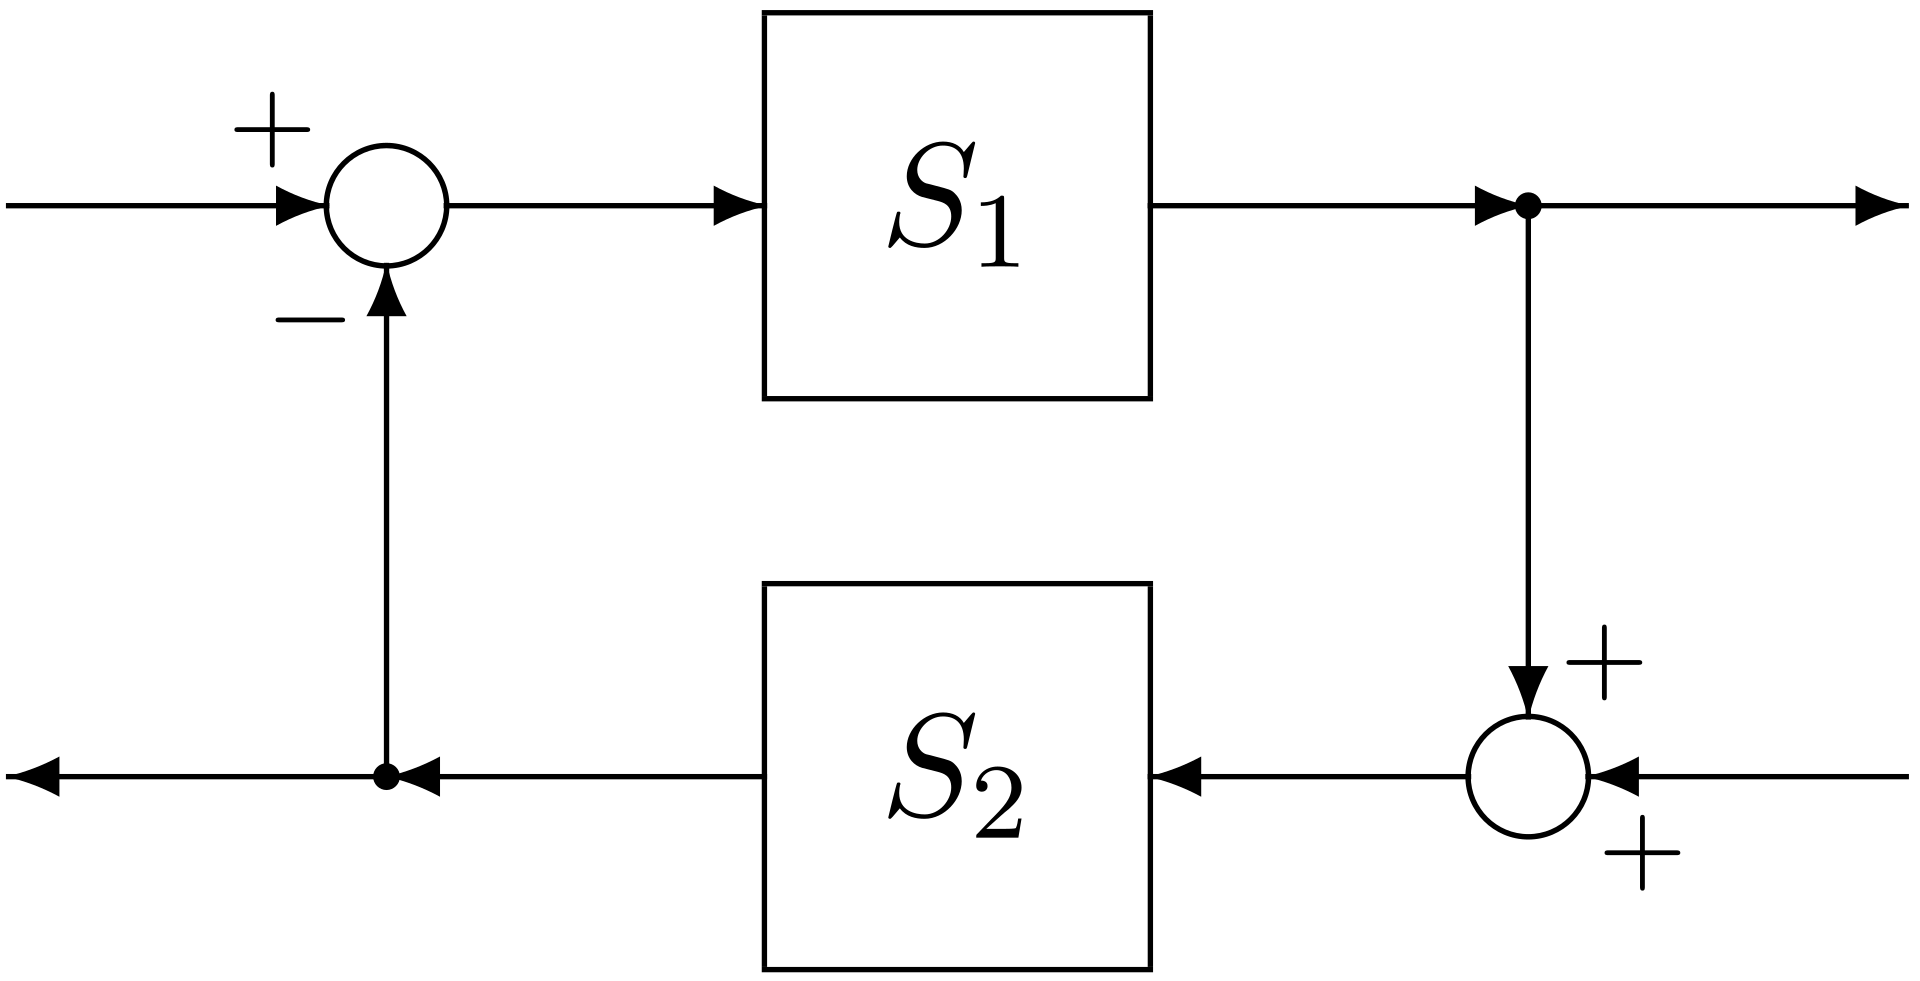
\includegraphics[scale=0.12]{img/small_gain.png}
    \end{figure}
    
    \begin{theorem}[Small-Gain Theorem]
        Suppose $S_1$ and $S_2$ are stable. Then, the interconnected system shown in the figure is well-posed and internally stable if and only if 
        \begin{equation}
            \Vert S_1 S_2 \Vert_\infty < 1
        \end{equation}
 \end{theorem}
    \noindent{
        \small{
            \textsf{See \Cref{p:Appendix}, \Cref{ch: SMT_example} for an example.}
        }
    } 
    
\end{multicols}

\subsection{Small-gain theorem in DDDC}
Since the plant is unknown, any attempt to describe the uncertainty affecting the plant leads to an \textbf{indirect data-driven control} problem. As we gave anticipated we describe the uncertainty as if it was on the controller and in particular: the \textit{ideal controller $K$*} plays the role of the nominal plant, while the uncertainty is given by the \textit{distance between the actual and ideal controller}.

\begin{figure}
    \centering
    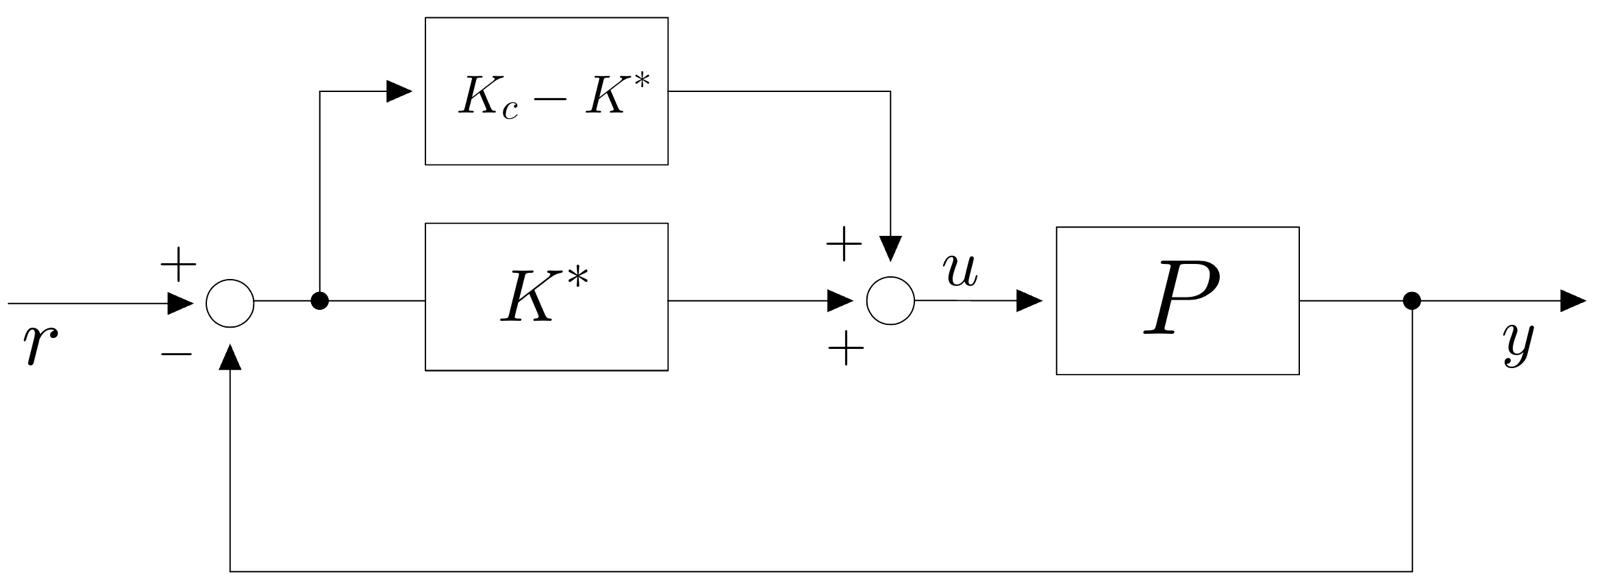
\includegraphics[scale=0.25]{img/SMT_DDDC.jpg}
    \caption{Uncertain description of the controller}
\end{figure}

\noindent
In this context the \textit{Small-gain theorem} can be applied where the subsystems $S_1$ and $S_2$ are defined as:
\begin{equation}
    S_1 = K_c-K^*, \quad S_2=\frac{-P}{1+K^*P}
\end{equation}
The following important theorem is given (whose proof can be retrieved from \cite{van2011data}):
\begin{theorem}\label{th:stab}[\Citeauthor{van2011data}, \citeyear{van2011data})]
    Let
    \begin{equation}\label{eq:def_Delta}
        \Delta(z)=M(z)-K_c(z)P(z)(1-M(z))
    \end{equation}
    the controller $K_c$ stabilizes the plant $P$ if
    \begin{enumerate}
        \itemsep-0.2em
        \item The ideal controller $K^*=\frac{M}{P(1-M)}$ stabilizes the plant; 
        \item $\Delta(z)$ is stable;
        \item $\Vert \Delta(z) \Vert_\infty<1$
    \end{enumerate}
\end{theorem}

\noindent
At this point, we can say that: (i) Condition 1 is satisfied if $M$ is stable and no unstable cancellations occur; (ii) Condition 2 is satisfied if both $P$ and $M$ are stable. But, \textbf{How to compute $\Vert \Delta(z) \Vert_\infty$ without using the plant and given noisy data?} The following section is aimed to answer to this question.

\subsection{Set-Membership estimation of $\Vert \Delta(z) \Vert_\infty$}
A three-steps procedure can be used, in order to obtain frequency by frequency a worst-case estimate on $\vert \Delta(e^{i\omega}) \vert$. 

\subsubsection{First step: a-priori information on $\Delta$}
The system $\Delta(z)$ can be generally defined as
\begin{equation}\label{eq:delta_q}
    \Delta(q^{-1}) = \frac{
        \gamma_0 + \gamma_1 q^{-1} + \dots + \gamma_{n_\Delta} q^{-n_{\Delta}}
    }{
        1+\delta_1 q^{-1} + \dots + \delta_{n_{\Delta}} q^{-n_\Delta}
    }
\end{equation}
from the definition of $\Delta$ we can say that $n_\Delta \le n_K + n_P +  n_M$, where $K, P, M$ are respectively the central controller, the plant and the reference model. Moreover using \Cref{eq:def_Delta}, and multiplying both sides by $r(k)$ you can get rid of the unknown plant
\begin{align}
    &\Delta(q^{-1}) r(k) = M(q^{-1}) r(k) - K_c(q^{-1}) (1-M(q^{-1})) 
    \overbrace{P(q^{-1}) r(k)}^{y(k)=\tilde{y}(k)-\eta(k)}\\
    &\Delta(q^{-1}) r(k) = M(q^{-1}) r(k) - K_c(q^{-1}) (1-M(q^{-1})) 
    {[\tilde{y}(k)-\eta(k)]}=\\
    &=Mr(k)-K_c(1-M)\tilde{y(k)} + K_c(1-M)\eta(k)=\\
    &=z(k) + F(q^{-1}) \eta(k) \label{eq:lastmaxdelta}
\end{align}
Here the samples of $z(k)$ can be obtained by simulation, while $F(q^{-1})$ is completely known.

\subsubsection{Second step: worst-case norm estimation problem}
For a fixed frequency $\omega$ a worst-case norm estimation can be obtained as:
\begin{equation}\label{eq:original_Delta_prob}
    \begin{aligned}
        &\max_{\Delta,\eta} \vert \Delta(e^{i\omega}) \vert\\
        &{\text{s.t.}}\\
        &\Delta(q^{-1})r(k) = z(k) + F(q^{-1})\eta(k)\\
        &\vert \eta(k) \vert \le \Delta_\eta
    \end{aligned}
\end{equation}

\subsubsection{Third step: obtaining a POP}
With a non-negligiblle effort the problem in \cref{eq:original_Delta_prob} can be recasted into a POP. At first we can note that $\Delta(e^{i\omega})$ is nothing but a complex number that can be written as
\begin{equation}\label{eq:complex}
    \Delta(e^{i\omega})=a+ib
\end{equation}
we are interested in the magnitude of such a number, that is: 
\begin{equation}\label{eq:norm}
    \vert \Delta(e^{i\omega}) \vert = \sqrt{a^2+b^2} \iff \exists{t}: t=\vert \Delta(e^{i\omega}) \vert, \ t^2=a^2+b^2
\end{equation}
The powers of the numbers $e^{ik\omega}$, $k=0,...,n_\Delta$ can be written in cartesian form as: 
\begin{equation}
    \begin{bmatrix}
        e^{in_\Delta{\omega}}\\
        \vdots\\
        e^{i2\omega}\\
        e^{i\omega}\\
        e^0\\
    \end{bmatrix}=\begin{bmatrix}
        \rho_0\\\rho_1\\\rho_2\\\vdots\\\rho_{n_\Delta}
    \end{bmatrix}+ i \begin{bmatrix}
        \sigma_0\\\sigma_1\\\sigma_2\\\vdots\\\sigma_{n_\Delta}
    \end{bmatrix}
\end{equation}
As a \textbf{function of the parameters $\gamma,\delta$} we can evaluate $\Delta(e^{i\omega})$ and estabilish a relation between $a,b,\gamma,\delta$ as:
\begin{align}
    &\Delta(z=e^{i\omega})=\frac{
        \gamma_0{e^{i{n_\Delta}\omega}}+\gamma_1 e^{i(n_\Delta-1)\omega}+\dots+\gamma_{n_\Delta-1} e^{i\omega}+\gamma_{n_\Delta}
    }{
        \delta_0 {e^{i{n_\Delta}\omega}}+
        \delta_1 e^{i(n_\Delta-1)\omega}+
        \dots + 
        \delta_{n_\Delta-1}e^{i\omega}+
        \delta_{n_\Delta}
    }=a+ib\\
    &\sum_{j=0}^{n_\Delta} \gamma_j e^{i(n_\Delta-j)\omega} = (a+ib)
    \sum_{j=0}^{n_\Delta} \delta_j e^{i(n_\Delta-j)\omega}\label{eq:dgab}
\end{align}
We have assumed that $\delta_0=1$ in order to simplify the notation. Replacing the cartesian form of the complex numbers $e^{i(n_\Delta-j)\omega}$ we obtain: 
\begin{equation}
    \sum_{j=0}^{n_\Delta} \gamma_j (\rho_j+\sigma_j) = (a+ib)
    \sum_{j=0}^{n_\Delta} \delta_j (\rho_j+\sigma_j)
\end{equation}
\noindent
By separating real and imaginary parts we obtain:
\begin{equation}
    \sum_{j=0}^{n_\Delta} \gamma_j \rho_j + i \gamma_j\sigma_j = 
    \sum_{j=0}^{n_\Delta}{
        a \delta_j \rho_j + i a \delta_j \sigma_j + i  b \delta_j \rho_j - b \delta_j \sigma_j
    }
\end{equation}
The two sides are equal if and only if the real parts are equal each other, the same for the imaginary parts, then two equations are obtained: 
\begin{align}
    &\sum_{j=0}^{n_\Delta} {\color{red}\gamma_j} \rho_j= \sum_{j=0}^{n_\Delta}{
         {\color{red}a\delta_j} \rho_j  -  {\color{red}b\delta_j} \sigma_j 
    } \quad \textsf{Real parts}\label{eq:real}\\ 
    &\sum_{j=0}^{n_\Delta} {\color{red}\gamma_j} \sigma_j= \sum_{j=0}^{n_\Delta}{
        {\color{red}a \delta_j} \sigma_j  + {\color{red}b \delta_j} \rho_j 
    } \quad \textsf{Imaginary parts}\label{eq:img}
\end{align}

\noindent
In {\color{red}red} the optimization variables, $\sigma_j$ and $\rho_j$ are known numbers. Next, $\gamma,\delta$ are related to the data and noise samples according to: $$\Delta(q^{-1}) r(k)=z(k) + F(q^{-1}) \eta(k)$$
In the following we are using  $r_k$ instead of $r(k)$ to ease the notation. Then, by using the definition of $\Delta$ and being $n_F$ and $\alpha_j^F, \ \beta_j^F$, respectively the number of parameters and the parameters of $F(q^{-1})$, we can obtain:
\begin{align}
    &\frac{
        \sum_{j=0}^{n_\Delta} \gamma_j q^{-j}
    }{
        \sum_{j=0}^{n_\Delta} \delta_j q^{-j}
    }r_k = z_k +  \frac{
        \sum_{j=0}^{n_F} \beta_j^F q^{-j}
    }{
        \sum_{j=0}^{n_F} \alpha_j^F q^{-j}
    } \eta_k \qquad \textsf{Removing the denominators...}\label{eq:first_1}\\
    &
    \bigg(\sum_{j=0}^{n_F} \alpha_j^F q^{-j}\bigg) 
    \bigg(\sum_{j=0}^{n_\Delta} \gamma_j q^{-j}\bigg) r_k=
    \bigg(\sum_{j=0}^{n_F} \alpha_j^F q^{-j}\bigg) 
    \bigg(\sum_{j=0}^{n_\Delta} \delta_j q^{-j}\bigg) r_k + 
    \bigg(\sum_{j=0}^{n_F} \beta_j^F q^{-j}\bigg) \bigg(\sum_{j=0}^{n_\Delta} \delta_j q^{-j}\bigg) \eta_k \label{eq:plain_eq} \\
    &\bigg(
        \sum_{j=0}^{n_F} \sum_{h=0}^{n_\Delta} {\alpha_j^F \gamma_h q^{-j-h}}
    \bigg) r_k =
    \bigg(
        \sum_{j=0}^{n_F} \sum_{h=0}^{n_\Delta}{\alpha_j^F \delta_h q^{-j-h}} 
        \bigg) 
    r_k+
        \sum_{j=0}^{n_F} \sum_{h=0}^{n_\Delta}{\beta_j^F \delta_h q^{-j-h}}
     \eta_k\label{eq:lastbutone}\\
     &
        \sum_{j=0}^{n_F} \sum_{h=0}^{n_\Delta} {\alpha_j^F {\color{red}\gamma_h} \ r({k-j-h})} =
        \sum_{j=0}^{n_F} \sum_{h=0}^{n_\Delta}{\alpha_j^F {\color{red}\delta_h} \ r({k-j-h})} +
        \sum_{j=0}^{n_F} \sum_{h=0}^{n_\Delta}{\beta_j^F {\color{red}\delta_h} \ \eta({k-j-h})}\label{eq:last_one}
\end{align}
\subsubsection{Summing up... (\textit{Don't loose ourself!})}
A lot of boring computations have been done, in order to fix the ideas and clarify the steps, let us summarizing what we have done keeping in mind that our main focus was to obtain a POP starting from the problem in \Cref{eq:original_Delta_prob}:
\begin{enumerate}
    \item A generic complex number can be described by \Cref{eq:complex}, and its norm  is given by \Cref{eq:norm}, this leads to the definition of the slack variables $a,b,t$ for real and imaginary part and for the magnitude of $\Delta(e^{i\omega})$;
    \item The description of $\Delta$ has been provided in \Cref{eq:delta_q} in function of its parameters ($\gamma,\delta$), exploiting the relationship $q\to{z}$, and evaluating it in $e^{i\omega}$ we have obtained the \Cref{eq:dgab} which relates $a,b,\gamma,\delta$. In order to complete this first block of transformation, equations \cref{eq:real} and \cref{eq:img} have been obtained; 
    \item Exploiting the expression of $\Delta(q^{-1})$ in \Cref{eq:delta_q} and using the final step \cref{eq:lastmaxdelta} we can obtain a relation between $\gamma,\delta$ and the collected data $\{r_k,\tilde{y}_k\}$; 
    \item This leads to the equation \Cref{eq:first_1} in which we have put everything together and in order to unify the notation we have expressed also $F(q^{-1})$ in function of its parameters ($\alpha^F, \beta^F$); 
    \item Multiplying both sides for the denominators of a term and the other the expression in \cref{eq:plain_eq} has been obtained. To collect all the terms involving the backward-shift operator nested summations are used in \Cref{eq:lastbutone} step; 
    \item The backward-shift operator property has been applied in order to obtain the \Cref{eq:last_one}, which relates the parameters of the $\Delta(q^{-1})$ with the experimentally collected data. To conclude note that all of the parameters of F($q^{-1}$) can be easily obtained since both $K_c$ and $M$ are also known at this stage.
 \end{enumerate}

We are ready! Overall, the optimization problem is recast to:

\begin{equation}\label{eq:final_problem}
    \begin{aligned}
        &\max_{t,a,b\in\mathbb{R}, \gamma\in\mathbb{R}^{n_\Delta+1}, 
    \delta\in\mathbb{R}^{n_\Delta}, \eta\in\mathbb{R}^N} {t}\\
    &\text{s.t.}\\
    &t^2=a^2+b^2\\
    &\sum_{j=0}^{n_\Delta} {\color{black}\gamma_j} \rho_j= \sum_{j=0}^{n_\Delta}{
        {\color{black}a\delta_j} \rho_j  -  {\color{black}b\delta_j} \sigma_j 
   }\\
   &\sum_{j=0}^{n_\Delta} {\color{black}\gamma_j} \sigma_j= \sum_{j=0}^{n_\Delta}{
       {\color{black}a \delta_j} \sigma_j  + {\color{black}b \delta_j} \rho_j 
   }\\
   &\sum_{j=0}^{n_F} \sum_{h=0}^{n_\Delta} {\alpha_j^F {\color{black}\gamma_h} \ r_{k-j-h}} =\\
        &=\sum_{j=0}^{n_F} \sum_{h=0}^{n_\Delta}{\alpha_j^F {\color{black}\delta_h} \ r_{k-j-h}} +
        \sum_{j=0}^{n_F} \sum_{h=0}^{n_\Delta}{\beta_j^F {\color{black}\delta_h} \ \eta_{k-j-h}}\\
    &\vert \eta(k) \vert \le \Delta_\eta
    \end{aligned}
\end{equation}

By solving this problem by using convex SDP relaxation a bound on the true $\vert\Delta(e^{i\omega})\vert$ can be found. Theoretically since at the end we have to find an $\mathcal{H}_\infty$-norm, the problem (\ref{eq:final_problem}) must be solved for all $\omega\in[0,2\pi]$. Alternatively, to simplify an already complicated problem, we can introduce a Lipshitz continuity assumption on $\vert \Delta(e^{i\omega})\vert$, assuming that it does not increase or decay faster than a certain $L_b=100$dB/dec or $L_b=200$dB/dec. Finally, after having computed the bound on a certain number of frequencies, you take the max, such a value gives you an estimate of the searched quantity $\Vert \Delta(z) \Vert_\infty$. For more details you can refer to the paper \cite{abuabiah2023non}, in which you can find these results and others in the MIMO case.\\

\noindent
To conclude this discussion, \textit{What if the Condition 3 of the \Cref{th:stab} is not satisfied?} A possible way to solve this problem is to collect a larger amount of experimental data so that the size of the FCPS is reduced. In this way the distance between the central estimate and the ideal controller becomes smaller, and in turn, $\Vert \Delta \Vert_\infty$ decreases.


\section*{References}
\begin{itemize}
    \itemsep-0.3em
    \item[\Large{\ding{45}}]  \Citeauthor{cerone2017direct}, \textit{\citetitle{cerone2017direct}}, \citedate{cerone2017direct}
    \item[\Large{\ding{45}}]  \Citeauthor{abuabiah2023non}, \textit{\citetitle{abuabiah2023non}}, \citedate{abuabiah2023non}
    \item[\Large{\ding{45}}]  \Citeauthor{van2011data}, \textit{\citetitle{van2011data}}, \citedate{van2011data}
\end{itemize}







\chapter[$\mathcal{H}_\infty$ approch for reference model in DDDC]{Model selection for Direct data-driven control through $\mathcal{H}_\infty$ techniques}
Here the objective is to describe a systematic approach by which a \textit{Reference Model} $M(q^{-1})$, that can be used in the framework of DDDC, can be obtained given suitable \textit{quantitative performance requirements}. In the literature (see \citeauthor*{campestrini2016unbiased} \cite{campestrini2016unbiased} and \citeauthor*{da2018choice} \cite{da2018choice}) several valid guidelines are provided about this topic, however they do not explicitly take into account for performance requirements.

\begin{figure}[h]
    \centering
    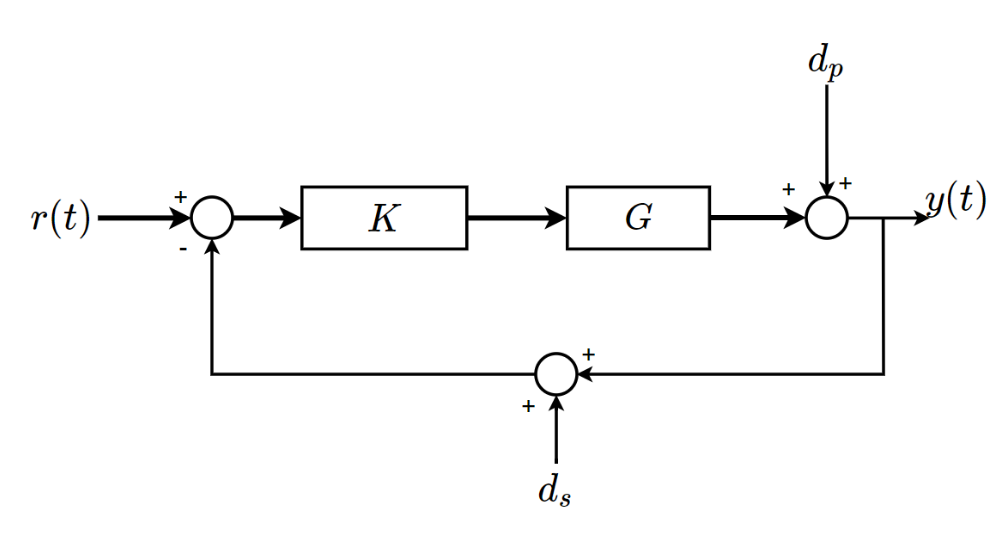
\includegraphics[scale=0.3]{img/RefMod_1.png}
    \caption{General FCS with disturbance and reference}
    \label{fig: gen_FCS}
\end{figure}

In general, we want to find a reference model $M$ that is able to take into account both tracking and disturbance/noise rejection. \\
\textit{Standard approaches} which address the problem of designing a reference model, are aimed to impose a certain behaviour to the complementary sensitivity function $T(q^{-1})$ of the system in \Cref{fig: gen_FCS}. For example:
\begin{itemize}
    \item \textsf{Prototype I Order System} the step response can be obtain, in the frequency domain, as 
    \begin{equation}\label{eq:prot_first}
        M(s)=\frac{1}{1+\frac{s}{p}}
    \end{equation}
    the time constant $1/p$ is the only degree of freedom which is used in order to obtain faster/slower rise time, in this case no oscillations and overshoot occur.
     \item \textsf{Prototype II Order System} We aim at building a reference model $M$ as follows: 
     \begin{equation}\label{eq:prot_second}
        M(s)=\frac{\omega_n^2}{s^2+2\zeta\omega_n{s}+\omega_n^2}
     \end{equation}
     here according to the parameter $\zeta$ different damping properties can be obtained (oscillations in the step response), the time constant $1/{\zeta\omega_n}$ is tuned in order to obtain certain convergence properties.
\end{itemize}

\noindent
It seems that all the needed performances can be achieved by properly tuning the parameters of such prototype models. However, it is remarkable that the input/output behaviour of the feedback control system in \Cref{fig: gen_FCS} is given by: 
\begin{equation}
    y=Tr+S{d_p}+T{d_s}
\end{equation}
Even if the function $S(q^{-1})=1-T(q^{-1})$ directly depends on the complementary sensitivity function whose shape can be decided using \Cref{eq:prot_first} and \Cref{eq:prot_second}, it is not said at all that it enjoys good attenuation properties with respect to the disturbance $d_p(t)$ acting on the plant! \\
The \textbf{proposed approach} is to design $M(q^{-1})$ by solving a fictitious control design problem accounting for all the quantitative performance requirements involved in the considered control problem.

\section{Model reference design: the $\mathcal{H}_\infty$ approach}
Here we consider the problem of designing $M(q^{-1})$ by solving a fictitious control problem in the framework of the $\mathcal{H}_\infty$ optimization (see \citeauthor*{cerone2020h} \cite{cerone2020h}). Common classes of \textbf{quantitative performance requirements} are: 
\begin{itemize}
    \itemsep-0.3em
    \item steady-state response to polynomial reference inputs
    \item steady-state response to polynomial disturbance $d_p$ 
    \item steady-state response to measurement disturbance $d_s$
    \item transient step response requirements in term of: rise time $t_r$, settling time $t_{s,\alpha\%}$ and overshoot $\hat{s}$.    
\end{itemize}
It is well known that in the context of $\mathcal{H}_\infty$ control, performance requirements can be translated into frequency domain constraints on a \textbf{weighted} $\mathcal{H}_\infty$-norm on the sensitivity function ($S$) and complementary sensitivity function ($T$):
\begin{align}
    \Vert W_T(j\omega) T(j\omega) \Vert_\infty \le 1\\
    \Vert W_S(j\omega) S(j\omega) \Vert_\infty \le 1
\end{align}

\subsection{Case 1: stable and minimum phase plant}
When the unknown plant is stable and minimum phase the problem of finding a reference model $M(s)$ is given by:
\begin{equation}
    M(s)=\tilde{T}(s)=\frac{\tilde{K}(s)\tilde{G}(s)}{1+\tilde{K}(s)\tilde{G}(s)}
\end{equation}
where $\tilde{K}(s)$ is the controller obtained by solving the optimization problem:
\begin{equation}
    \tilde{K}(s)=\arg\min_{\tilde{K}\in \tilde{K}(s)^{stab}} {\Vert T_{wz}(s)} \Vert_\infty
\end{equation}
where $T_{wz}$ is the closed  loop transfer function between the input $w$ and the output $z$, and $W_S$ and $W_T$ are rational transfer function designed taking into account frequency domain constraints imposed by performance requirements, that is
\begin{equation}
    T_{wz}(s)=\begin{bmatrix}
        W_T \tilde{T}\\
        W_S \tilde{S}
    \end{bmatrix}
\end{equation}
the block-diagram of the general control configuration we are referring to is the one depicted in \Cref{fig:gen_plant} which is the generalized plant for \textit{nominal performance requirements}.

\begin{figure}[h]
    \centering
    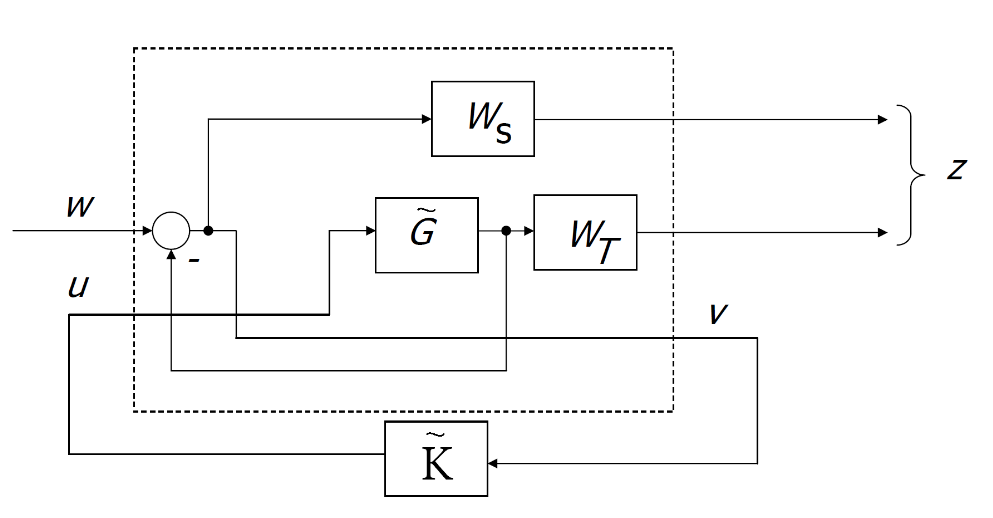
\includegraphics[scale=0.35]{img/gen_plant.png}
    \caption{Generalized plant for nominal performances}
    \label{fig:gen_plant}
\end{figure}
\begin{remark}
    The controller $\tilde{K}$ is instrumental to the computation of $\tilde{T}$ and then the reference model $M$. In other words the controller $\tilde{K}$ does not solve the problem for the actual plant which is unknown.
\end{remark}

\subsection{Case 2: stablle non-minimum phase systems}
\begin{definition}[\textbf{Non-minimum phase system}]
    
A non-minimum phase system is a dynamic system whose transfer function has one or more zeros in the right-half of the s-plane (for continuous-time systems) or outside the unit circle (for discrete-time systems). These zeros lead to certain undesirable characteristics, particularly in transient response and stability.
\end{definition}

Step-response of non-minimum phase exhibit \textit{undershoot}, in particular it is a behaviour of  the transient response of a system where the output initially moves in the direction opposite to the desired final value before eventually settling at the target.\\

In this case, the reference model can be designed using the $\mathcal{H}_\infty$ approach, but instead of selecting $\tilde{G}=1$ as fictitious plant, we include all the NMP zeros of the plant a number of poles equals or greater than the NMP ones. The additional poles are chosen in arbitrary way\footnote{
    It is well-known that stable poles do not induce any performance limitation in the feedback control system.
} under the condition that they are stable, moreover if the system type is greater or equal than one a suitable number of poles at the origin can be included in $\tilde{G}$.

\subsection{Last step: Discretization of $M(s)$}
Since in the DDDC based on the SM approach, we use a discrete-time description, the reference model is supposed to be discretized using a suitable sampling time $T_s$, obtaining then the reference model $M(q^{-1})$

\section{Simulation example and discussion}
In this example, we use the proposed approach to tune a controller for a SISO NMP plant. A numerical comparison with the standard approach is presented. Here we assume that the plant is a NMP system described by the following transfer function
\begin{equation}
    G(s)=\frac{(s+9.925)(s-1.818)}{(s+12.04)(s+2.231)}
\end{equation}
the disturbances are
\begin{equation}
    \begin{aligned}
        &d_p(t)=a_p\sin(\omega_p{t}), \ \vert a_p \vert \le 2\cdot{10^{-2}}, \ \omega_p \le 0.02 \text{rad \ s}^{-1}\\
        &d_s(t)=a_s\sin(\omega_s{t}), \ \vert a_s \vert \le {10^{-1}}, \ \omega_s \le 40 \ \text{rad \ s}^{-1}\\
    \end{aligned}
\end{equation}

The \Cref{tab:performance} reports the time domain specifications and the performances achieved with the contrrolled systems obtained with the two approaches (SMRC) and ($\mathcal{H}_\infty$RMC).

\begin{table}[h!]
\centering
\begin{tabular}{|>{\raggedright\arraybackslash}m{5cm}|>{\centering\arraybackslash}m{3cm}|>{\centering\arraybackslash}m{3cm}|>{\centering\arraybackslash}m{3cm}|}
\hline
\textbf{Performance Specifications} & \textbf{Upper Bound Value} & \textbf{SRMC} & \textbf{$H_\infty$RMC} \\ \hline
Steady-state output error when the reference is a ramp & 0.5 & \textbf{0.7} & 0.495 \\ \hline
Steady-state output error in the presence of $d_p$ & $6 \cdot 10^{-4}$ & $2.84 \cdot 10^{-4}$ & $2.22 \cdot 10^{-4}$ \\ \hline
Steady-state output error in the presence of $d_s$ & $8 \cdot 10^{-3}$ & \textbf{0.0196} & $6.83 \cdot 10^{-3}$ \\ \hline
Step response overshoot & 11\% & \textbf{11.5\%} & 9.77\% \\ \hline
Rise time & 2 (s) & 0.939 (s) & 0.988 (s) \\ \hline
Settling time & 8 (s) & 6.36 (s) & 7.33 (s) \\ \hline
\end{tabular}
\caption{Performance Comparison}
\label{tab:performance}
\end{table}

It is remarkable that even if the two step-responses are quite similar, the controlled system designed by using the standard approach does not fulfill all the requirements, on the contrary the proposed approach fulfills all of the performance requirements.

\section*{References}
\begin{itemize}
    \itemsep-0.3em
    \item[\Large{\ding{45}}]  \Citeauthor{da2018choice}, \textit{\citetitle{da2018choice}}, \citedate{da2018choice}
    \item[\Large{\ding{45}}]  \Citeauthor{campestrini2016unbiased}, \textit{\citetitle{campestrini2016unbiased}}, \citedate{campestrini2016unbiased}
    \item[\Large{\ding{45}}]  \Citeauthor{cerone2020h}, \textit{\citetitle{cerone2020h}}, \citedate{cerone2020h}
\end{itemize}


\begin{comment}
\part{Appendix}
\chapter{Lab 1: Least-Squares parameter estimation (Solution)}

In this problem we assume that the plant is a continuous time LTI dynamical system assumed
to be exactly described by the following transfer function:

\begin{equation*}
    G_p(s) = \frac{100}{s^2+1.2s+1}
\end{equation*}

\begin{lstlisting}[style=Matlab-editor]  
    G=100/(s^2+1.2*s+1);
\end{lstlisting}

\noindent
Assuming that the input-output data have been collected with a sample time of Ts = 1s,
compute a discrete-time model for the plant as follows (see help of the Matlab command
\texttt{c2d}): $G_d(z)=\textsf{c2d}(G_p,1,\text{'zoh'})$:

\begin{lstlisting}[style=Matlab-editor]  
    Gz=c2d(G,1,'zoh'); 
\end{lstlisting}

\noindent
Use the obtained discrete-time model to generate input-output data by applying to the system
a randomsequence of $N$ samples and amplitude 1 as input (see commands rand and command
\texttt{lsim}). Collect the input sequence in the array $u$ and the output sequence in the array $w$.

\begin{lstlisting}[style=Matlab-editor]    
    n=2; 
    k=n+1;              %Point where I have to start
    H=1e5+n;            %I need at least (3n+1) samples
            
    u=rand(H, 1);
    %noisy-data (Equation Error)
    w_nf=lsim(Gz,u);
\end{lstlisting}

\section{Noise-Free experiment}
\noindent
Using the array u and w, build matrix A and array b required for the computation of the least
squares estimate of the discrete-time model parameters, according to the theory and examples
about least square estimation presented in the classroom.

\begin{lstlisting}[style=Matlab-editor] 
    [numGz, denGz]=tfdata(Gz,'v');
    th_true = [denGz(2:end) numGz]'

    A = [-w_nf(2:H-1) -w_nf(1:(H-2)) u(3:H) u(2:(H-1)) u(1:(H-2))];
    th_est_noise_free = A\w_nf(k:H)
\end{lstlisting}

\section{Equation-Error setting}
Repeat the exercise (for different values of $N$) by adding a random \textit{equation error} $e$ while
simulating the data.

\begin{lstlisting}[style=Matlab-editor] 
    D=tf([0 0 1],denGz,1);
    e = 5*randn(H,1);
    w_nEE = lsim(Gz,u)+lsim(D,e);
    A = [-w_nEE(2:H-1) -w_nEE(1:(H-2)) u(3:H) u(2:(H-1)) u(1:(H-2))];
    th_est_noiseEE = A\w_nEE(k:H) 
\end{lstlisting}

\section{Output-Error setting}
Repeat the exercise (for different values of $N$) by adding a random \textit{output measurement error}
$\eta$.

\begin{lstlisting}[style=Matlab-editor] 
    %simulation in case of Output-Error(OE) setting
    std=5;
    eta=std*randn(H,1);
    w_nOE=lsim(Gz,u)+eta;

    A = [-w_nOE(2:H-1) -w_nOE(1:(H-2)) u(3:H) u(2:(H-1)) u(1:(H-2))];
    th_est_noiseOE = A\w_nOE(k:H)
\end{lstlisting}




\chapter[L2: PUI with EE noise structure]{Lab2: FPS and PUI with Equation-Error noise structure}

In this problem we assume that the plant to be identified is exactly described as a discrete-time LTI model described by the following transfer function:
\end{comment}

\newpage
\printbibliography


\end{document}